\documentclass[11pt, a4paper]{article}

% --- PDFLATEX-COMPATIBLE PREAMBLE BLOCK ---
\usepackage[a4paper, top=2.5cm, bottom=2.5cm, left=2cm, right=2cm]{geometry}
\usepackage[T1]{fontenc}
\usepackage[utf8]{inputenc}
\usepackage[english]{babel}
\usepackage{newtxtext}

\usepackage{authblk} % Standard package for author affiliations
\usepackage{graphicx}
\usepackage{multirow}
\usepackage{amsmath,amssymb,amsfonts}
\usepackage{amsthm}
\usepackage{newtxmath}
\usepackage{mathrsfs}
\usepackage[title]{appendix}
\usepackage[table]{xcolor}
\usepackage{textcomp}
\usepackage{booktabs}
\usepackage{array}
\usepackage{caption}
\usepackage{makecell}
\usepackage{adjustbox}
\usepackage{rotating}
\usepackage{pdflscape}
\usepackage{placeins}
\usepackage{algorithm}
\usepackage{algorithmicx}
\usepackage{algpseudocode}
\usepackage{listings}
\usepackage[hidelinks]{hyperref}
\usepackage{orcidlink}
\usepackage[table]{xcolor}
\usepackage{booktabs,multirow,makecell,threeparttable,graphicx}
\theoremstyle{plain}
\newtheorem{theorem}{Theorem}
\newtheorem{proposition}[theorem]{Proposition}
\usepackage{arydshln}
\newcommand{\NA}{\textemdash}

\theoremstyle{definition}
\newtheorem{example}{Example}
\newtheorem{remark}{Remark}
\newtheorem{definition}{Definition}
\raggedbottom

\begin{document}

\title{Structured Weak-Oracle Semantic Prior Learning for LLM-Augmented Cross-Modal Cervical Disease Analytics}

\author[1]{Mengyuan Huang~\orcidlink{0000-0003-2478-480X}\thanks{yuanmeng\_h@mails.ccnu.edu.cn}}
\author[1,2]{Yuchen Pei~\orcidlink{0000-0002-1506-1979}\thanks{ycpei@ccnu.edu.cn}}
\author[3]{Yan Zhang~\orcidlink{0009-0008-5997-2724}\thanks{Corresponding author. RM002125@whu.edu.cn}}
\author[1,2]{Yutao Ma~\orcidlink{0000-0003-4239-2009}\thanks{Corresponding author. ytma@ccnu.edu.cn}}

\affil[1]{School of Computer Science, Central China Normal University, Wuhan 430079, Hubei, China}
\affil[2]{Hubei Provincial Key Laboratory of Artificial Intelligence and Smart Learning, Central China Normal University, Wuhan 430079, Hubei, China}
\affil[3]{Department of Obstetrics and Gynecology, Renmin Hospital of Wuhan University, Wuhan 430060, Hubei, China}

\maketitle

\begin{abstract}

\textbf{Background:}
Large-scale cervical screening generates multimodal imaging and clinical evidence, but clinician-authored reports are often incomplete and unevenly distributed across centres, limiting cohort use and semantic auditability.

\textbf{Methods:}
We developed MOSAIC (Multicentre Offline Structured Anchoring with Imbalanced-report Calibration), a leakage-controlled framework that converts incomplete report supervision into quality-controlled weak semantic priors. MOSAIC combines large language model-assisted structured pseudo-report completion, section-aware report-anchored alignment, and a train-only semantic retrieval bank with validation-calibrated logit fusion. Generated text is used only as weak semantic supervision and is not treated as clinical ground truth. We evaluated 1,897 multimodal cases from five centres with 137,591 evaluable image files; 744 cases had archived reports and 1,153 were pseudo-report candidates.

\textbf{Results:}
On the locked held-out test set, MOSAIC achieved AUROC 0.908, AUPRC 0.741, and F1 0.736, compared with AUROC 0.856 and F1 0.519 for the same backbone without retrieval calibration. Paired bootstrap analysis showed an AUROC gain of 0.053 over the backbone (95\% CI, 0.012--0.101; \(p=0.005\)). MOSAIC had a higher point estimate than the strongest same-split contrastive baseline, although this difference was not statistically conclusive.

\textbf{Conclusions:}
MOSAIC reframes incomplete clinical-report supervision as an auditable semantic-prior learning problem for retrospective multimodal analytics. The findings support weak-oracle completion, section-aware alignment, and leakage-controlled retrieval calibration, but do not establish prospective clinical use or autonomous large language model decision-making.

\vspace{1em}
\noindent\textbf{Keywords:} cervical screening; multimodal learning; report supervision imbalance; semantic alignment; big data

\end{abstract}


\section{Introduction}
\label{sec:introduction}



%--overview
% \begin{figure}
%     \centering
%     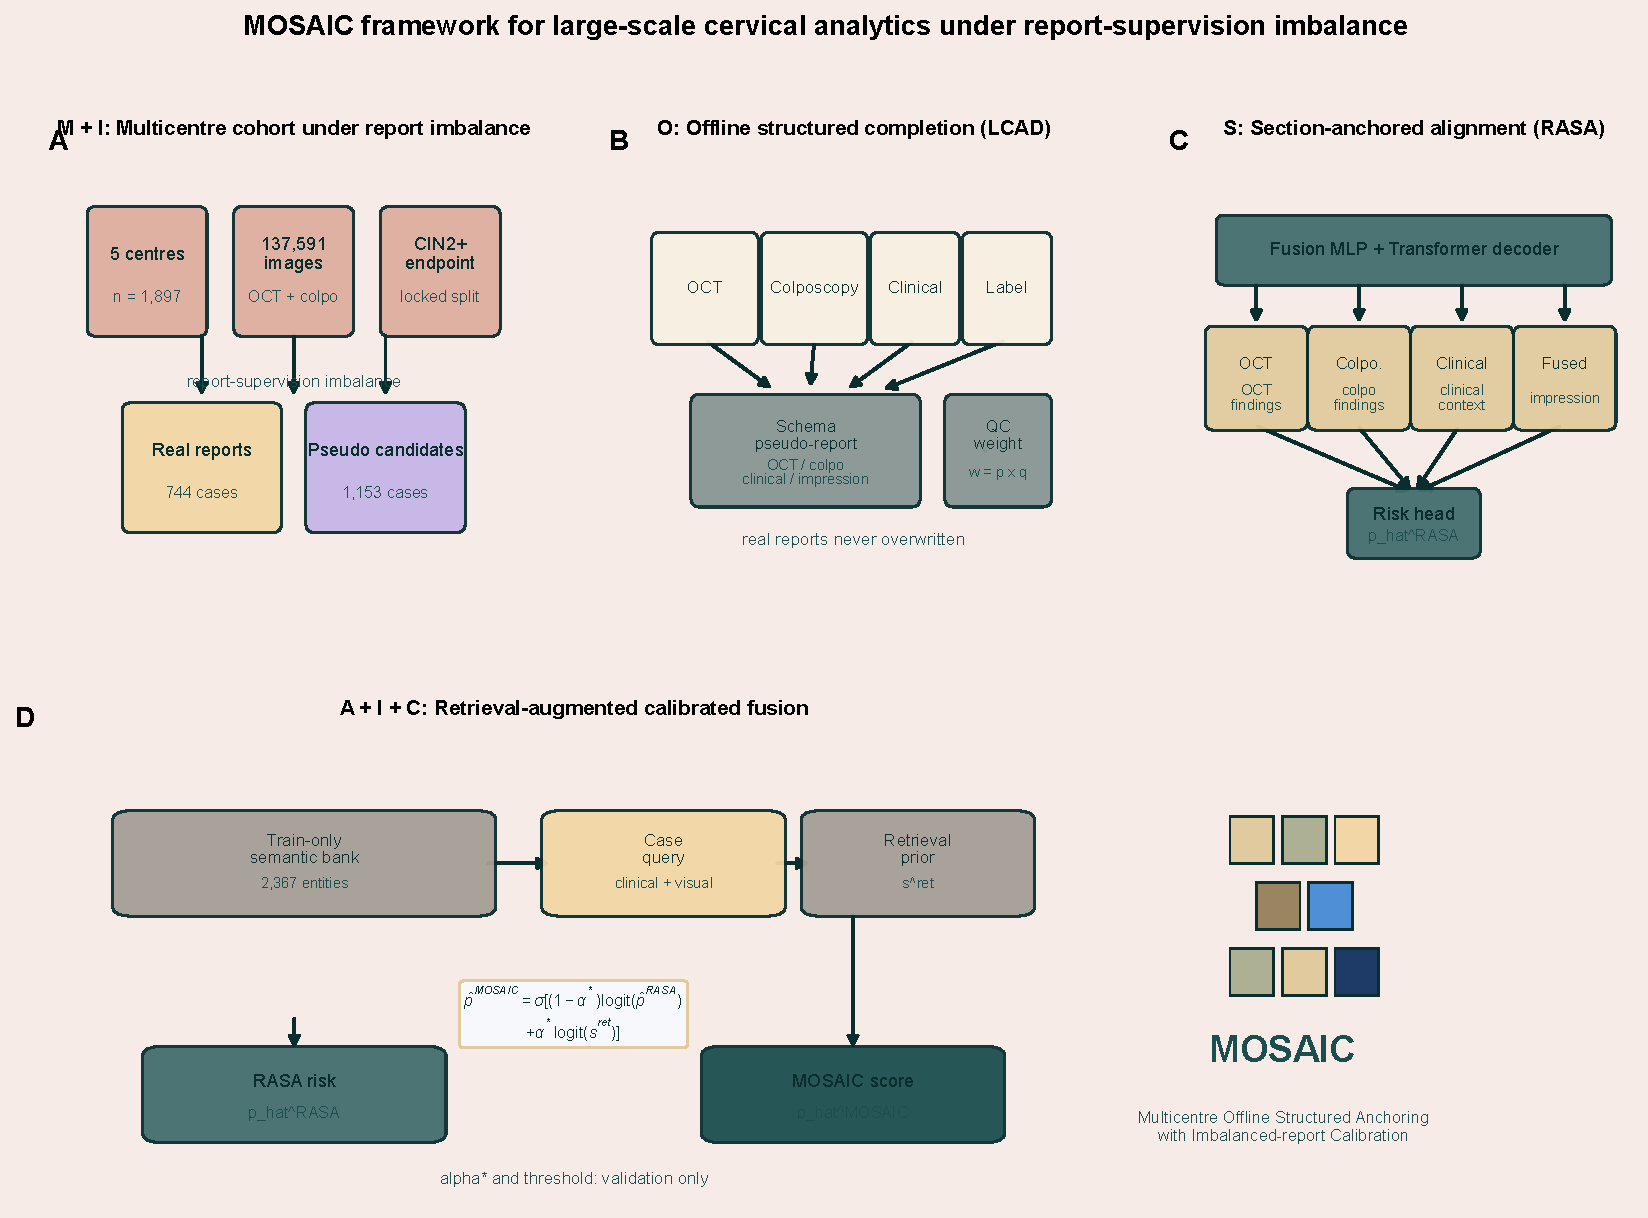
\includegraphics[width=1\linewidth]{final_Fig/Figure1_mosaic_overview.pdf}
%     \caption{Overview of the MOSAIC framework (Multicentre Offline Structured Anchoring with Imbalanced-report Calibration).
%     (A) Five-center cohort construction and case-level report-supervision imbalance.
%     (B) Offline structured completion for report-missing cases through schema-constrained LCAD pseudo reports and QC weighting.
%     (C) Section-anchored RASA alignment between OCT, colposcopy, clinical instruction, fused visual evidence, and structured report sections, with a CIN2+ risk head.
%     (D) Train-only semantic retrieval bank and validation-calibrated logit fusion that yields the final MOSAIC risk score.
%     The name MOSAIC refers both to the colposcopic mosaic pattern and to assembling fragmented multimodal and report-level evidence into a coherent semantic representation.}
%     \label{fig:mosaic_overview}
% \end{figure}


Cervical cancer prevention is moving from early-stage screening toward risk-adapted diagnostic pathways in which virology tests, cytology, colposcopy, optical coherence tomography (OCT)~\cite{huang1991oct}, histopathology, and clinical context are interpreted together. This shift is clinically necessary because the global elimination agenda and contemporary management guidelines for cervical cancer both emphasize risk stratification, timely treatment of precancerous diseases, and more precise post-screening management~\cite{who2020global_strategy,canfell2020mortality,perkins2020asccp}. Yet the shift also causes a more challenging analytics problem. In the routine workflow of cervical examination, many women with abnormal or positive screening results are referred for further evaluation; still, only a subset of them ultimately present high-grade cervical lesions. Such a procedure increases examinee anxiety, while also incurring unnecessary medical costs and prolonging examination time. The practical challenge of effectively detecting ``real'' patients is, therefore, to integrate heterogeneous evidence from various medical tests at scale while preserving clinically meaningful links among image findings, structured variables, report semantics, and diagnostic reasoning.

This clinical problem has motivated two broad streams of medical artificial intelligence (AI) research. One focuses on multimodal biomedical modeling, showing that medical images, structured records, clinical text, time-series signals, and other data types can provide complementary information for patient-level prediction~\cite{acosta2022multimodal,moor2023gmai,tu2024generalist_biomedical_ai}. More recent large-scale benchmarks and fusion architectures have further emphasized that clinical AI systems should rather operate across heterogeneous data sources than rely on a single modality~\cite{dai2025climb,aljorf2025medpatch}. The other focuses on medical report generation and vision--language learning, where textual reports are used to connect visual observations with clinically interpretable descriptions~\cite{monshi2020radiology_reports,pang2023medical_report_generation,gu2026radalign}. Together, these studies suggest that scalable clinical analytics should not only fuse multimodal features but also exploit the semantic structure through which physicians describe, organize, and justify diagnostic evidence.

However, the conditions assumed by multimodal AI systems in gynecology differ from those encountered in real-world clinical environments. In previous studies and curated benchmarks, visual inputs, structured variables, diagnostic labels, and report-level annotations are often treated as if they were available with comparable completeness. Instead, this assumption rarely holds for cervical cancer detection in multicenter clinical settings. Imaging data and structured clinical variables may be collected at scale, whereas medical reports are center-dependent, non-standardized, and even incomplete. As a result, conventional report-generation or report-guided learning pipelines face a restrictive choice: training on the subset with complete textual supervision, or excluding report-missing cases from semantic representation learning. This data-use pattern reduces the effective cohort size, thereby reinforcing center-specific documentation bias, as report availability and style often reflect local workflows rather than underlying disease biology.

The resulting gap is more specific than a generic missing-modality problem. Existing multimodal AI models have sought to address sparse clinical inputs and missing data by leveraging weak supervision, which provides a general paradigm for learning from noisy or indirect labels~\cite{aljorf2025medpatch,ratner2020snorkel}. Nevertheless, incomplete report-level supervision poses an additional semantic problem: the missing element is not merely an additional input, but a structured clinical description that links modality-specific observations to diagnostic interpretation. Existing report-generation research has improved image-to-text modeling, but it usually relies on available medical reports as textual ground truth and pays less attention to settings where report supervision is institutionally imbalanced~\cite{monshi2020radiology_reports,pang2023medical_report_generation}. In this context, large language models (LLMs)~\cite{vaswani2017attention,brown2020language} bridge multimodal evidence and report-level semantics by structuring heterogeneous clinical observations into section-level textual representations, which can serve as language-mediated weak supervision when complete physician-authored reports are unavailable~\cite{hager2024llm_limitations,thirunavukarasu2023large}. Despite their promising performance, LLM-based medical AI systems should not be treated as autonomous diagnostic authorities in realistic clinical workflows due to hallucination and other issues~\cite{thirunavukarasu2023llm_medicine}. What remains insufficiently explained is how report-level semantics can serve as a controlled learning signal when real medical reports are sparse, uneven, and only partially accessible.

To address this gap in medical AI for cervical cancer detection, we formulate incomplete clinical report supervision as a weak-oracle prior-learning problem for large-scale multimodal cervical lesion analytics. In this formulation, report-like semantic targets may be constructed from available multimodal evidence and weak diagnostic labels; still, they are explicitly quality-gated and are not treated as physician-authored ground truth. Based on this formulation, we propose MOSAIC (\textbf{M}ulticenter \textbf{O}ffline \textbf{S}tructured \textbf{A}nchoring with \textbf{I}mbalanced-report \textbf{C}alibration), an LLM-augmented framework for cervical disease risk prediction under incomplete report-level supervision. Its name reflects the methodological objective of assembling fragmented multimodal and report-level evidence into a coherent semantic representation through LLM-assisted report structuring and controlled weak semantic supervision.

In this study, MOSAIC is organized into a three-stage chain of evidence to convert incomplete clinical-report supervision into auditable weak semantic priors. The first stage addresses report-level supervision imbalance through \textbf{L}abel-\textbf{C}onstrained, \textbf{A}uditable, and \textbf{D}ata-grounded pseudo-report completion (LCAD). LCAD performs offline, schema-constrained pseudo-report completion for report-missing cases and assigns quality-control weights, so that generated reports can provide bounded semantic targets without being treated as ground-truth annotations. The second stage introduces \textbf{R}eport-\textbf{A}nchored \textbf{S}ection \textbf{A}lignment (RASA), which decomposes structured reports into section-level semantic anchors corresponding to OCT findings, colposcopy findings, clinical context, and diagnostic expressions. These anchors are then used to guide modality-specific representation learning and to make the learned cross-modal associations inspectable at the section level. The third stage tests whether the learned semantic structure can contribute to risk prediction beyond what the basic representation alone can. A semantic memory bank is constructed solely from training cases, and retrieved semantic priors are integrated with the RASA backbone via validation-calibrated logit fusion to produce the final risk score. In this design, report-missing cases are not discarded; their generated semantic targets remain quality-controlled, confined to training-time supervision and retrieval, and available for audit.

%这段可以放到 MOSAIC 方法的概述中，或者删掉，intro部分不需要重复介绍
%The key methodological premise of MOSAIC is that LLM-derived report structure should function as a controlled semantic scaffold rather than as a substitute for clinical documentation or diagnostic judgment. LCAD allows report-missing multimodal cases to participate in representation learning without assuming equivalence between pseudo reports and clinician-authored reports. RASA further uses section-wise report anchors to encourage OCT, colposcopy, and structured clinical embeddings to support the corresponding clinical semantics. This alignment is not intended to establish formal topological equivalence, causal identification, or autonomous diagnostic reasoning. Instead, it provides a learnable and auditable mechanism for organizing heterogeneous multimodal evidence around clinically meaningful report sections. In this sense, MOSAIC instantiates LLM-augmented cross-modal semantic alignment for large-scale analytics: language-model-derived structure is used as a quality-controlled weak-supervision resource for scalable multimodal learning, while pathology-derived endpoints remain the basis for risk evaluation.

%重构这段文字，把贡献用 itemize 的形式列出来
% We evaluate MOSAIC on a privately curated five-center multimodal cervical examination cohort comprising OCT images, colposcopy images, structured HPV, TCT, and age variables, histopathology-derived endpoints, and incomplete report-level supervision. To our knowledge, this is among the first multicenter resources that enable report-aware cervical OCT analytics under realistic documentation imbalance, where imaging, structured clinical variables, pathological outcomes, and textual evidence are jointly available but unevenly distributed across institutions. MOSAIC uses this setting to recast incomplete-report supervision as weak-oracle semantic-prior learning. Rather than discarding report-missing cases, it converts them into quality-weighted semantic supervision through QC-gated pseudo-report completion, organizes multimodal representations with section-aware RASA anchors, and tests the resulting report-derived priors through train-only semantic retrieval and validation-calibrated fusion. The design maintains a strict boundary between generated text, clinician-authored reports, and pathology-derived endpoints, while a dedicated audit protocol evaluates report scarcity, source dependence, perturbation robustness, semantic tags, negative controls, and cross-center generalization. This combination of a rare multimodal cohort, bounded weak semantic supervision, and leakage-conscious retrieval makes MOSAIC a controlled framework for large-scale cervical screening analytics under imbalanced report supervision.

We evaluate MOSAIC on a privately curated five-centre multimodal cervical screening cohort that integrates OCT images, colposcopy images, structured human papillomavirus (HPV), thin-prep cytologic test (TCT), and age variables, pathology-harmonised endpoints, and incomplete report-level supervision. This setting exposes a practical but underexplored problem in large-scale clinical analytics: visual and structured evidence can be collected at scale, whereas report supervision remains sparse, centre-dependent, and unevenly documented. The core question is therefore not simply how to handle a missing modality, but how to convert incomplete report supervision into auditable weak semantic priors for cross-modal representation learning without treating generated text as clinical ground truth.

Built on this setting, the study makes three main contributions:
\begin{itemize}
\item \textbf{A report-aware multimodal cervical OCT analytics setting under realistic supervision imbalance.}
We construct a privately curated five-centre cohort that jointly contains OCT images, colposcopy images, structured HPV/TCT/age variables, pathology-harmonized endpoints, and incomplete clinician-authored report supervision. To our knowledge, this represents one of the first multicentre resources for report-aware cervical OCT analytics in which imaging, structured clinical variables, pathological evidence, and textual supervision are linked at the case level but unevenly available across institutions.

\item \textbf{A weak-oracle framework for LLM-augmented cross-modal semantic alignment.}
We formulate incomplete and centre-dependent report supervision as a weak-oracle semantic-prior learning problem. MOSAIC operationalises this formulation through label-constrained, data-grounded, and QC-gated pseudo-report completion, followed by RASA section anchoring. This design uses LLM-assisted report structuring as a controlled semantic scaffold, enabling OCT, colposcopy, structured clinical variables, and diagnostic-impression representations to be aligned with clinically meaningful report sections.

\item \textbf{A leakage-controlled retrieval-calibrated pipeline with bounded audit evidence.}
MOSAIC builds a semantic memory bank from training cases only and integrates retrieved report-derived priors with the RASA backbone through validation-calibrated logit fusion. The framework preserves a strict boundary between generated text, clinician-authored reports, and pathology-harmonised endpoints. Its evaluation combines same-split baselines, pseudo-report source comparisons, report-scarcity analysis, section-alignment ablations, perturbation sensitivity, semantic-tag controls, negative controls, centre-shift stress testing, and efficiency audits, supporting MOSAIC as a retrospective large-scale analytics framework rather than an autonomous diagnostic system.
\end{itemize}


The remainder of this article is organized as follows. Section~\ref{sec:related_work} reviews the related work of our study. Section~\ref{sec:methods} details the MOSAIC framework and its core components. Section~\ref{sec:experiments_results} presents experiment settings and reports cross-center prediction results of MOSAIC and baseline approaches. Section~\ref{sec:discussion} discusses the implications of our work for large-scale multimodal cervical lesion analytics, together with limitations related to retrospective validation, pseudo-report supervision, semantic retrieval, and clinical deployment. Finally, Section~\ref{sec:con} concludes this article and outlines our future work.

\section{Related Work}
\label{sec:related_work}

Report-aware multimodal clinical analytics connects several lines of research. One line studies multimodal clinical fusion, where images, structured variables, and clinical text are integrated for patient-level prediction. A second line studies medical report generation, where clinical reports are treated as structured textual outputs derived from medical evidence. A third line studies vision--language alignment and retrieval-enhanced modeling, where reports are used not only as outputs, but also as sources of supervision, semantic grounding, or external memory. MOSAIC is positioned at the intersection of these lines. Its focus, however, is more specific: real clinical reports are incomplete and unevenly distributed across centers, yet they contain semantic information that is too valuable to ignore.

\subsection{Multimodal clinical analytics under incomplete supervision}

Multimodal clinical learning is motivated by the fact that clinical decisions rarely rely on a single source of evidence. Images, structured records, clinical text, and other patient-level signals often provide complementary information for diagnosis and prognosis~\cite{acosta2022multimodal}. Recent generalist biomedical AI frameworks further argue that clinical models should support diverse data types and tasks, rather than remain limited to narrow single-modality settings~\cite{moor2023gmai,tu2024generalist_biomedical_ai}. Large-scale benchmark efforts such as CLIMB also reflect this shift, as they evaluate models across heterogeneous clinical inputs and tasks~\cite{dai2025climb}. In parallel, sparse- and missing-modality fusion methods, including MedPatch-style approaches, have addressed the practical problem that not all modalities are available for every case~\cite{aljorf2025medpatch}.

These studies provide an important foundation for multimodal clinical analytics, but they do not fully address report-supervision imbalance. In most missing-modality settings, the absent element is another input stream, such as an image view, a laboratory value, or a clinical note. In the present setting, the missing element is different. A missing report means that the model loses a structured semantic bridge between modality-specific findings and diagnostic interpretation. Removing report-missing cases would reduce the cohort scale and weaken multicenter learning. Treating generated reports as clinician-authored ground truth would introduce a different risk: uncontrolled semantic bias. This motivates a supervision-aware formulation, in which incomplete reports can guide representation learning only when their uncertainty is explicitly controlled.

\subsection{Medical report generation and LLM-augmented clinical text structuring}

Medical report generation has mainly been studied as an image-to-text task, especially in radiology. Early and recent methods have used encoder--decoder networks, attention mechanisms, memory modules, and transformer-based architectures to improve report fluency and clinical coverage~\cite{monshi2020radiology_reports,pang2023medical_report_generation}. Later work introduced disease-aware prompts, prototype memories, large language models, and retrieval-grounded generation to improve factuality and clinical specificity. Methods such as RadAlign further combine concept alignment, report generation, and retrieval-style grounding, strengthening the connection between visual evidence and clinical language~\cite{gu2026radalign}.

This literature shows that reports can encode clinically meaningful semantics. However, most report-generation methods still assume that paired reports are available as reliable training targets. This assumption is more suitable for curated radiology benchmarks than for multicentre screening cohorts, where report availability often depends on local documentation practice. In such cohorts, the central question is not how to generate standalone reports. The more relevant question is how incomplete report-level semantics can support multimodal learning without being treated as verified clinical truth.

LLMs provide a useful bridge in this setting. They can structure heterogeneous clinical observations into section-level textual representations, which can serve as language-mediated weak supervision when complete clinician-authored reports are unavailable. Weak supervision offers the broader methodological principle: noisy or indirect labels can support learning when their reliability is modeled rather than ignored~\cite{ratner2020snorkel}. At the same time, medical LLM studies caution that language-model outputs require workflow constraints, validation, and human oversight before they can influence clinical decision-making~\cite{thirunavukarasu2023llm_medicine}. MOSAIC follows this boundary. It does not use pseudo reports as clinical ground truth. Instead, LCAD constructs schema-constrained pseudo reports, assigns quality-control weights, and keeps pseudo reports distinct from clinician-authored reports.

\subsection{Report-derived cross-modal semantic alignment}

Vision--language alignment has shown that paired medical images and reports can produce clinically meaningful representations. Reports often describe findings, uncertainty, and interpretation patterns that are not fully captured by image-level labels. Medical image--text pretraining has therefore moved from global contrastive alignment toward local--global matching, disease-aware grounding, prototype learning, and knowledge-enhanced representation learning. These methods establish an important premise: reports can serve as semantic supervision, not merely as textual outputs.

However, many alignment methods still operate at the level of whole reports, global image--text pairs, image regions, or disease entities. This formulation is not always sufficient for multimodal cervical screening. OCT, colposcopy, and structured clinical variables carry different types of evidence. OCT reflects microstructural tissue patterns. Colposcopy reflects surface morphology and vascular changes. Clinical variables provide risk priors and management context. A single global report embedding may obscure this division of evidence.

These observations suggest that report structure should not be treated as a monolithic text target. For multimodal cervical screening, a more suitable formulation is to use report sections as modality-aware semantic anchors. In this formulation, each modality can be aligned with the report component it is expected to support. This motivates section-aware representation learning rather than generic image--text similarity learning, and it provides a more auditable link between modality-specific embeddings and clinically interpretable semantics.

\subsection{Retrieval-enhanced semantic memory and positioning of MOSAIC}

Retrieval-enhanced modeling has become a common strategy for improving factual grounding, interpretability, and long-tail generalization. In language modeling, retrieval-augmented generation and non-parametric memory allow models to leverage external examples rather than relying solely on parametric knowledge. In medical report generation, retrieval can provide similar cases, factual report fragments, or disease-aware references, which may improve clinical completeness and reduce hallucination.

MOSAIC uses retrieval in a more constrained way. Its retrieval bank contains training cases only, and validation and test labels are excluded from bank construction. At inference, the model retrieves semantically similar training evidence and converts it into a retrieval-derived risk prior. This prior is then combined with the RASA backbone through validation-calibrated logit fusion. The purpose is not to retrieve an answer from the test set, nor to replace the predictive model with case lookup. The purpose is to make the learned semantic space useful, auditable, and protected against label leakage.

Overall, prior work has established the value of multimodal clinical fusion, report-guided representation learning, LLM-assisted clinical text structuring, and retrieval-enhanced grounding. However, these directions rarely address settings in which report supervision is incomplete, center-dependent, and semantically useful yet unreliable as ground truth. MOSAIC is designed for this gap. It provides a controlled pathway for converting incomplete clinical report semantics into auditable weak supervision for large-scale cross-modal cervical screening analytics. The contribution therefore does not lie in simply adding an LLM, a report decoder, or a retrieval module to a multimodal classifier, but in defining how incomplete report-level semantics can be used without treating generated text as clinician-authored truth.







\section{Methods}
\label{sec:methods}

MOSAIC was designed to use incomplete clinical-report supervision without treating generated text as clinical ground truth. This section first defines the retrospective cohort, weak-oracle supervision target, and permitted evidence streams. It then describes the three linked modules of the framework: LCAD for QC-gated pseudo-report completion in report-missing cases, RASA for report-section-aware multimodal representation learning, and train-only semantic retrieval with validation-calibrated fusion for the final risk score. The remaining subsections specify the auxiliary LLM source audits, training objective, baseline and ablation design, perturbation and center-shift analyses, statistical protocol, and reproducibility controls that support the experimental evaluation in Section~\ref{sec:experiments_results}.

\subsection{Retrospective Design and Weak-Oracle Formulation}
\label{subsec:methods_design}




We formulated this study as a five-centre retrospective multimodal learning problem under \emph{report-supervision imbalance}. The distinctive big-data challenge is that visual and clinical evidence are available at scale, whereas clinician-authored report supervision is sparse, centre-dependent, and not missing at random. Thus, the learning target is not only a diagnostic risk function, but also a controlled mechanism for converting incomplete report-level semantics into auditable weak supervision.

Let
\begin{equation}
\mathcal{D}=\{(x_i^{oct},x_i^{col},x_i^{fus},x_i^{clin},y_i,c_i,a_i,r_i^{real})\}_{i=1}^{N},
\end{equation}
where \(N=1897\), \(y_i\in\{0,1\}\) is the harmonised CIN2+ supervision label, \(c_i\) is the centre identifier, \(a_i=\mathbb{I}(r_i^{real}\ \mathrm{available})\) is the report-availability indicator, and \(x_i^{oct}\), \(x_i^{col}\), \(x_i^{fus}\), and \(x_i^{clin}\) denote OCT, colposcopy, fused visual, and structured clinical evidence. The clinical vector \(x_i^{clin}\) was derived from permitted non-identifying clinical variables such as HPV status, TCT/cytology category, age, and other structured screening fields. Centre identifiers were used for stratification, report-availability analysis, and centre-shift evaluation, but were not used as predictive input features. The report-supervision imbalance is characterized by the centre-conditional availability distribution
\begin{equation}
\pi_c=\Pr(a_i=1\mid c_i=c),
\end{equation}
which varies strongly across centres and is therefore treated as part of the data-generating structure rather than as random annotation dropout.

The fixed split \((\mathcal{D}_{tr},\mathcal{D}_{val},\mathcal{D}_{te})\) was defined at case level. All representation learning and semantic-bank construction used \(\mathcal{D}_{tr}\) only; \(\mathcal{D}_{val}\) was used for fusion-weight and threshold selection; \(\mathcal{D}_{te}\) was reserved for held-out evaluation. Held-out test labels were never used for pseudo-report generation, semantic retrieval-bank construction, calibration, thresholding, or model selection.

The method follows the same evidence chain used in the experimental section. First, LCAD converts report-missing training cases into QC-weighted weak semantic supervision. Second, RASA uses structured report sections as modality-aware semantic anchors for multimodal representation learning. Third, train-only semantic retrieval converts the learned report space into a retrieval prior that is fused with the RASA backbone using validation-selected calibration. This order is important: generated text is used to shape representations and retrieval priors, while the locked CIN2+ endpoint remains the basis for predictive evaluation.



% MOSAIC compact pseudocode for main text
% Requires: \usepackage{algorithm,algorithmic}
%---伪代码-----
\begin{algorithm}[htbp]
\small
\caption{MOSAIC retrospective protocol: weak-oracle completion, section-anchored learning, and retrieval-calibrated fusion}
\label{alg:mosaic_compact}
\begin{algorithmic}[1]

\State \textbf{Input:} cohort $\mathcal{D}=\{x_i^{oct},x_i^{col},x_i^{fus},x_i^{clin},c_i,y_i,r_i^{real}\}_{i=1}^{N}$;
splits $(\mathcal{D}_{tr},\mathcal{D}_{val},\mathcal{D}_{te})$; sections $\mathcal{K}$; thresholds $\mathcal{T}$; perturbations $\mathcal{M}$.
\State \textbf{Model:} encoders $P_{\{oct,col,fus,clin\}}$, fusion $F_\theta$, report encoder/decoder $(E_\theta,G_\theta)$, section heads $\{S_k\}$, risk head $W_r$.
\State \textbf{Hyperparameters:} $\eta,B,\theta_{QC},\lambda_{rep},\lambda_{sec},\lambda_{risk},\lambda_{cons}$.

\Statex \Comment{\textbf{LCAD: quality-controlled weak-oracle supervision}}
\For{$i\in\mathcal{D}_{tr}$}
    \If{$r_i^{real}$ exists}
        \State $r_i^\star\leftarrow r_i^{real}$,\quad $w_i\leftarrow1$.
    \Else
        \State $e_i\leftarrow\mathrm{ExtractEvidence}(x_i^{oct},x_i^{col},x_i^{clin})$,\quad
        $\tilde r_i\leftarrow G_{LCAD}(e_i,y_i)$.
        \State $(q_i,p_i,z_i)\leftarrow\mathrm{QC}(\tilde r_i,y_i,e_i)$,\quad
        $w_i\leftarrow p_iq_i\mathbb{I}(q_i\ge\theta_{QC})\mathbb{I}(z_i=0)$.
        \State If $w_i>0$, set $r_i^\star\leftarrow\tilde r_i$; otherwise drop $\tilde r_i$ from report-supervision losses.
    \EndIf
\EndFor
\State $\mathcal{D}_{tr}^{+}\leftarrow\{(i,r_i^\star,w_i):i\in\mathcal{D}_{tr},w_i>0\}$.

\Statex \Comment{\textbf{RASA: section-anchored multimodal optimization}}
\Repeat
    \For{mini-batch $\mathcal{C}\subset\mathcal{D}_{tr}^{+}$}
        \State $h_i\leftarrow F_\theta([P_{oct}(x_i^{oct});P_{col}(x_i^{col});P_{fus}(x_i^{fus});P_{clin}(x_i^{clin})])$.
        \State $H_i\leftarrow E_\theta(\mathrm{Tok}(r_i^\star),h_i)$,\quad
        $\hat r_i\leftarrow G_\theta(H_i)$,\quad
        $\hat p_i^{RASA}\leftarrow\sigma(W_rh_i)$,\quad
        $\{g_i^k\}\leftarrow\mathrm{SectionPool}(H_i)$.
        \State $\mathcal{L}\leftarrow
        \lambda_{rep}\sum_i w_i\mathrm{CE}(\hat r_i,r_i^\star)
        +\lambda_{sec}\sum_{i,k}[1-\cos(S_k(h_i),g_i^k)]
        +\lambda_{risk}\sum_i\mathrm{BCE}(\hat p_i^{RASA},y_i)
        +\lambda_{cons}\sum_i|\hat p_i^{RASA}-y_i|$.
        \State $\Theta\leftarrow\mathrm{AdamW}(\Theta,\nabla_\Theta\mathcal{L},\eta)$.
    \EndFor
\Until{convergence on $\mathcal{D}_{val}$}

\Statex \Comment{\textbf{Train-only semantic-prior retrieval}}
\State Build semantic bank $\mathcal{B}_{tr}$ from report sections in $\mathcal{D}_{tr}^{+}$ only.
\For{$i\in\mathcal{D}_{val}\cup\mathcal{D}_{te}$}
    \State $s_i^{ret}\leftarrow\mathrm{Retrieve}(\mathrm{ExtractEvidence}(x_i^{oct},x_i^{col},x_i^{clin}),\mathcal{B}_{tr})$,\quad
    $\hat p_i^{RASA}\leftarrow f_\Theta(x_i^{oct},x_i^{col},x_i^{fus},x_i^{clin})$.
\EndFor

\Statex \Comment{\textbf{Validation-calibrated fusion and test evaluation}}
\State $\alpha^\star\leftarrow\arg\max_{\alpha\in[0,1]}\mathrm{AUROC}\{\sigma[(1-\alpha)\mathrm{logit}(\hat p_i^{RASA})+\alpha\mathrm{logit}(s_i^{ret})],y_i;\mathcal{D}_{val}\}$.
\State $\hat p_i^{MOSAIC}\leftarrow\sigma[(1-\alpha^\star)\mathrm{logit}(\hat p_i^{RASA})+\alpha^\star\mathrm{logit}(s_i^{ret})]$.
\State $\tau^\star\leftarrow\arg\max_{\tau\in\mathcal{T}}\mathrm{F1}(\mathbb{I}[\hat p_i^{MOSAIC}\ge\tau],y_i;\mathcal{D}_{val})$.
\State Evaluate $\hat y_i=\mathbb{I}[\hat p_i^{MOSAIC}\ge\tau^\star]$ on $\mathcal{D}_{te}$; test labels are never used for $\alpha^\star$ or $\tau^\star$.

\Statex \Comment{\textbf{Perturbation and audit}}
\State For $m\in\mathcal{M}$ and $i\in\mathcal{D}_{te}$, compute perturbed outputs
$(\hat p_{i,m}^{RASA},\hat r_{i,m})$ 

and audit
$\Delta p_{i,m}=\hat p_{i,m}^{RASA}-\hat p_{i,0}^{RASA}$,
$\Delta s_{i,m}=1-\mathrm{Sim}(\hat r_{i,m},\hat r_{i,0})$.
\State \textbf{Output:} $\Theta^\star$, $\mathcal{D}_{tr}^{+}$, $\mathcal{B}_{tr}$, $\alpha^\star$, $\tau^\star$, held-out metrics, sensitivity audit, and perturbation statistics.

\end{algorithmic}
\end{algorithm}



\subsection{Permitted Evidence Encoding and Shared Representation}
\label{subsec:methods_encoding}

MOSAIC first maps the permitted multimodal evidence into a shared case representation. For each case, OCT, colposcopy, and fused visual evidence were represented using cached visual embeddings \(v_i^{oct},v_i^{col},v_i^{fus}\in\mathbb{R}^{2048}\), where \(v_i^{oct}\), \(v_i^{col}\), and \(v_i^{fus}\) denote the 2048-dimensional OCT, colposcopy, and fused visual embeddings for case \(i\), respectively. Structured clinical information was encoded as \(u_i\in\mathbb{R}^{32}\), where \(u_i\) denotes the 32-dimensional clinical instruction vector derived from permitted non-identifying clinical fields. Report text, centre identifiers, pathology-like variables, and outcome labels were not used as predictive input features.

Each evidence stream was projected into a shared hidden space:
\begin{equation}
\begin{aligned}
h_i^{oct} &= W_{oct}v_i^{oct}+b_{oct}, &
h_i^{col} &= W_{col}v_i^{col}+b_{col},\\
h_i^{fus} &= W_{fus}v_i^{fus}+b_{fus}, &
h_i^{clin} &= W_{clin}u_i+b_{clin}.
\end{aligned}
\end{equation}
Here, \(h_i^{oct}\), \(h_i^{col}\), \(h_i^{fus}\), and \(h_i^{clin}\) are modality-specific hidden representations; \(W_{oct}\), \(W_{col}\), \(W_{fus}\), and \(W_{clin}\) are trainable projection matrices; and \(b_{oct}\), \(b_{col}\), \(b_{fus}\), and \(b_{clin}\) are bias terms. The projected representations were concatenated and passed through a fusion multilayer perceptron as \(h_i=F_{\theta}([h_i^{oct};h_i^{col};h_i^{fus};h_i^{clin}])\), where \(F_{\theta}(\cdot)\) is the fusion network with trainable parameters \(\theta\), \([\cdot]\) denotes vector concatenation, and \(h_i\) is the fused case-level representation. This representation was shared by the structured report decoder, section-alignment heads, and CIN2+ risk-prediction head.

\subsection{Report-Supervision Imbalance and Weak-Oracle Targets}
\label{subsec:methods_report_imbalance}

After multimodal evidence encoding, report availability was modelled explicitly. Let \(\mathcal{R}=\{i:a_i=1\}\) denote cases with archived reports and \(\mathcal{P}=\{i:a_i=0\}\) denote report-missing pseudo-report candidates. Instead of excluding \(\mathcal{P}\), MOSAIC constructs a QC-gated weak-oracle supervision target:
\begin{equation}
r_i^{\star}
=
\begin{cases}
r_i^{real}, & a_i=1,\\
G_{\mathrm{LCAD}}(e_i,y_i;\mathcal{S}), & a_i=0\ \mathrm{and}\ \omega_i>0,
\end{cases}
\end{equation}
where \(e_i=\mathrm{ExtractEvidence}(x_i^{oct},x_i^{col},x_i^{clin})\), \(\mathcal{S}\) is the fixed structured-report schema, and \(G_{\mathrm{LCAD}}\) is the local structured completion function. The associated supervision weight is
\begin{equation}
\omega_i
=
a_i
+
(1-a_i)p_iq_i\mathbb{I}(q_i\geq\theta_{\mathrm{QC}})\mathbb{I}(z_i=0),
\end{equation}
where \(p_i\) is generator confidence, \(q_i\) is the QC score, \(\theta_{\mathrm{QC}}\) is the QC threshold, and \(z_i=1\) indicates a severe contradiction or hallucination flag. The effective training set is therefore
\begin{equation}
\mathcal{D}_{tr}^{+}=\{(i,r_i^{\star},\omega_i):i\in\mathcal{D}_{tr},\omega_i>0\}.
\end{equation}
This construction is the weak-oracle component of MOSAIC: generated reports are not treated as physician-authored documentation, but as weighted semantic scaffolds that allow report-missing cases to contribute to representation learning.

\subsection{MOSAIC Architecture and Methodological Contributions}
\label{subsec:methods_mosaic}

MOSAIC integrates three linked methodological contributions. The first contribution is weak-oracle completion: report-missing cases are not discarded, but are assigned schema-constrained and QC-weighted semantic targets through LCAD. The second contribution is report-section anchoring: RASA decomposes each structured report into OCT findings, colposcopy findings, clinical context, and diagnostic impression, so that multimodal representations are aligned with clinically interpretable sections instead of a single opaque report embedding. The third contribution is leakage-controlled semantic memory: only training cases are inserted into the retrieval bank, and the final retrieval prior is fused with the RASA backbone using validation-selected calibration. These three components define the primary MOSAIC pipeline, while external provider runs, semantic-tag retrieval, and token-packer variants are treated as audits or ablations rather than as replacement definitions of the method.

\subsection{LCAD: QC-Gated Weak-Oracle Report Completion}
\label{subsec:methods_lcad}

For cases in \(\mathcal{P}\cap\mathcal{D}_{tr}\), structured pseudo reports were generated using LCAD. LCAD is the report-completion component of MOSAIC: it converts report-missing training cases into bounded semantic supervision while keeping real reports and pseudo reports explicitly separated. It used extracted multimodal evidence \(e_i\) and the harmonised CIN2+ supervision label to produce a schema-constrained report:
\begin{equation}
r_i^{pseudo}=G_{\mathrm{LCAD}}(e_i,y_i;\mathcal{S}),
\end{equation}
where \(G_{\mathrm{LCAD}}(\cdot)\) is the local structured generation function and \(\mathcal{S}\) is the fixed report schema. This generation step was used to construct training supervision only; held-out test labels were not used for pseudo-report generation or QC selection.

The generated report was decomposed into predefined sections, \(r_i^{pseudo}=\{s_i^{sum},s_i^{oct},s_i^{col},s_i^{clin},s_i^{imp},s_i^{rec}\}\). In this notation, \(s_i^{sum}\) is the diagnostic summary, \(s_i^{oct}\) is the OCT findings section, \(s_i^{col}\) is the colposcopy findings section, \(s_i^{clin}\) is the clinical context section, \(s_i^{imp}\) is the diagnostic impression, and \(s_i^{rec}\) is the recommendation section. The fixed schema was used to make pseudo-report supervision auditable and section-specific.

Each pseudo report was subjected to QC before entering \(\mathcal{D}_{tr}^{+}\). The final weak-oracle weight \(\omega_i\) follows the QC-gated definition in Section~\ref{subsec:methods_report_imbalance}: real reports receive \(\omega_i=1\), whereas pseudo reports receive a continuous weight only if they satisfy both quality and severe-error filters. The QC procedure assessed required-section completeness, label--impression consistency, unsupported high-grade or invasive-cancer terminology, hallucination under missing-modality conditions, sentence-level evidence, confidence validity, and privacy sanitisation. This design allowed report-missing cases to contribute weak semantic supervision while limiting the influence of unreliable pseudo reports.

\subsection{Bounded LLM Assistance and Source-Replacement Audit}
\label{subsec:methods_provider}

The main MOSAIC pipeline used local structured pseudo reports as QC-weighted weak semantic supervision. In a separate auxiliary analysis, we evaluated whether structured pseudo-report generation could be implemented by alternative sources under the same schema. These sources included a label-template baseline, a rule-based generator, a local embedding-assisted generator, and selected external API-based providers. Table~\ref{tab:llm_role_sources} summarises how each source was used. This distinction is central to the claim boundary: external API providers were not used as the default training supervision mechanism, and generated pseudo reports were not treated as clinician-authored ground truth.

For provider \(m\), the generated pseudo report was written as \(r_{i,m}^{api}=G_m(e_i;\mathcal{S})\), where \(r_{i,m}^{api}\) is the structured pseudo report generated for case \(i\) by provider \(m\), \(G_m(\cdot)\) is the provider-specific generation function, \(e_i\) is the de-identified structured evidence supplied to the provider, and \(\mathcal{S}\) is the fixed report schema. This provider comparison evaluated schema validity, section completeness, modality support, contradiction rate, hallucination rate, duplicate-text fraction, latency, and estimated cost. It was used to assess source substitutability and operational feasibility, not to define the main training pipeline.

External provider evaluations used only de-identified structured evidence. Raw images, image paths, patient names, internal patient identifiers, hospital names, and directly identifying information were not transmitted. In the current implementation, external providers are therefore treated as an auxiliary source-comparison experiment rather than as the default supervision mechanism for MOSAIC. The LLM component supplies structured semantic scaffolding for representation learning and audit; it is not an autonomous diagnostic decision-maker, and real reports are never overwritten by pseudo reports.

The external-provider audit was conducted as an auxiliary source-comparison analysis on training-split pseudo-report candidates. All providers were evaluated under the same fixed structured-report schema, label-constrained prompting mode, deterministic decoding setting, and de-identification protocol. The audit compared whether different API-accessible language models could produce schema-valid and modality-supported pseudo reports under the MOSAIC completion protocol. Only de-identified structured evidence was submitted; raw images, image paths, patient identifiers, hospital identifiers, and directly identifying information were excluded. This analysis was used to assess source replaceability and operational feasibility of the structured completion layer.

\begin{table*}[!htbp]
  \centering
  \caption{Structured pseudo-report sources and role of LLM augmentation in retrospective weak-oracle supervision.}
  \label{tab:llm_role_sources}
  \scriptsize
  \begin{threeparttable}
  \resizebox{\linewidth}{!}{%
  \begin{tabular}{p{3cm}ccp{2cm}p{2cm}p{3.8cm}p{4cm}}
    \toprule
    \textbf{Source} & \textbf{\makecell{Used in main\\MOSAIC training?}} & \textbf{\makecell{Auxiliary source\\comparison?}} & \textbf{Input evidence} & \textbf{Output format} & \textbf{De-identification/privacy status} & \textbf{Role in claim} \\
    \midrule
    Label template baseline & No & Yes & Weak label only & Structured schema fields & No external transmission & Negative control for schema-only text without modality grounding \\
    
    Rule-based generator & No & Yes & De-identified structured evidence & Structured pseudo report & Local only & Non-LLM structured baseline for source comparison \\
    
    Local embedding-assisted generator & Yes & Yes & De-identified OCT, colposcopy, clinical evidence features, and weak label constraints & Structured pseudo report & Local only & Primary weak-oracle semantic scaffold when archived reports are missing \\
    
    External API providers & No & Yes & De-identified structured evidence only & Structured pseudo report & Raw images, image paths, patient identifiers, hospital identifiers, and direct identifiers were not transmitted & Feasibility and source-replaceability audit only \\
    \bottomrule
  \end{tabular}%
  }
  % \begin{tablenotes}[flushleft]
  %   \footnotesize
  %   \item Pseudo reports are QC-weighted weak semantic scaffolds rather than clinical ground truth. External providers were evaluated only as auxiliary sources; their outputs do not define the main MOSAIC training pipeline.
  % \end{tablenotes}
  \end{threeparttable}
\end{table*}

\subsection{RASA: Report-Conditioned Backbone and Risk Head}
\label{subsec:methods_rasa}

RASA links the fused multimodal representation to both structured report decoding and CIN2+ risk prediction. It is the backbone used before retrieval calibration, and its role is to make report supervision operational at the section level rather than only at the case-label level. Let \(t_i=(t_{i,1},t_{i,2},\ldots,t_{i,L})\) denote the tokenised training report \(\tilde{r}_i\), where \(t_{i,l}\) is the \(l\)-th report token and \(L\) is the maximum report sequence length. The report-token embeddings were conditioned on the fused multimodal representation as \(\bar{e}_{i,l}=E(t_{i,l})+h_i\), where \(E(\cdot)\) is the token-embedding function, \(E(t_{i,l})\) is the embedding of token \(t_{i,l}\), and \(\bar{e}_{i,l}\) is the multimodal-conditioned token embedding at position \(l\).

The contextual report hidden states were computed using a transformer encoder:
\begin{equation}
H_i=
\mathrm{Transformer}_{\phi}(\bar{e}_{i,1},\bar{e}_{i,2},\ldots,\bar{e}_{i,L}),
\end{equation}
where \(H_i=(H_{i,1},H_{i,2},\ldots,H_{i,L})\) is the sequence of contextual hidden states, \(H_{i,l}\) is the hidden state at token position \(l\), and \(\phi\) denotes transformer parameters. Token-level logits were obtained as \(\hat{T}_{i,l}=W_{dec}H_{i,l}+b_{dec}\), where \(\hat{T}_{i,l}\) is the predicted logit vector over the report vocabulary at token position \(l\), and \(W_{dec}\) and \(b_{dec}\) are decoder parameters. The CIN2+ risk head mapped the fused representation to a case-level probability, \(\hat{p}_i=\sigma(W_{risk}h_i+b_{risk})\), where \(\hat{p}_i\) is the predicted CIN2+ probability for case \(i\), \(W_{risk}\) and \(b_{risk}\) are risk-head parameters, and \(\sigma(\cdot)\) is the sigmoid function.

\subsection{RASA Section-Wise Semantic Attractor Alignment}
\label{subsec:methods_section_alignment}

The central mechanism of RASA is to use structured report sections as semantic attractors for multimodal representation learning. The report hidden sequence was divided into section-level proxies \(g_i^k=\mathrm{Pool}_{k}(H_i)\) for \(k\in\mathcal{K}\), where \(\mathcal{K}=\{oct,col,clin,imp\}\) is the set of aligned report sections. The index \(k=oct\) corresponds to OCT findings, \(k=col\) to colposcopy findings, \(k=clin\) to clinical context, and \(k=imp\) to diagnostic impression. The term \(g_i^k\) denotes the hidden proxy for section \(k\), and \(\mathrm{Pool}_{k}(\cdot)\) denotes mean pooling over token positions assigned to that section. The fused representation was mapped into section-specific alignment spaces as \(a_i^{k}=A_k(h_i)\), where \(A_k(\cdot)\) is the projection head for section \(k\), and \(a_i^k\) is the projected representation used to align with the corresponding report-section proxy.

The section-alignment loss was defined as
\begin{equation}
\mathcal{L}_{align}
=
\frac{1}{B_{mb}|\mathcal{K}|}
\sum_{i=1}^{B_{mb}}
\sum_{k\in\mathcal{K}}
\left[
1-
\frac{a_i^{k}\cdot g_i^{k}}
{\|a_i^{k}\|_2\|g_i^{k}\|_2}
\right].
\end{equation}
Here, \(\mathcal{L}_{align}\) is the section-alignment loss, \(B_{mb}\) is the mini-batch size, \(|\mathcal{K}|\) is the number of aligned sections, \(a_i^k\cdot g_i^k\) is the inner product between the projected representation and the report-section proxy, and \(\|\cdot\|_2\) denotes the Euclidean norm. This loss encourages OCT evidence to align with OCT findings, colposcopy evidence with colposcopy findings, clinical information with clinical context, and fused multimodal evidence with diagnostic impression.

This alignment does not claim formal topological isomorphism or causal explanation. Instead, it imposes a topology-aware representation-learning constraint in which structured report sections act as modality-aware semantic attractors.

\subsection{Train-Only Semantic Retrieval and Validation-Calibrated Fusion}
\label{subsec:methods_retrieval_fusion}

To complete MOSAIC, we constructed a train-only cervical semantic bank \(\mathcal{B}_{tr}\). Each bank entity stored section text, modality tags, abnormality attributes, section embeddings, and the corresponding training-case weak-oracle risk indicator. For each validation or test case, OCT, colposcopy, fused visual, and clinical signatures queried \(\mathcal{B}_{tr}\) to retrieve section-wise semantic entities without using validation or test labels. The retrieved positive semantic prior \(s_i^{\mathrm{ret}}\) was then fused with the RASA backbone risk score. This retrieval-calibrated layer is the defining inference component of MOSAIC; the section-anchored backbone without retrieval calibration is referred to as MOSAIC-RASA.

The train-only semantic bank is
\begin{equation}
\mathcal{B}_{tr}
=
\{(b_j^k,\ell_j,k): j\in\mathcal{D}_{tr}^{+},\ k\in\mathcal{K}\},
\end{equation}
where \(b_j^k\) is the embedding of section \(k\) from case \(j\), and \(\ell_j\) is the training-case risk label or abnormality indicator used only inside the training bank. For a validation or test case \(i\), the retrieval weights are
\begin{equation}
\rho_{ij}^{k}
=
\frac{\exp(\mathrm{sim}(u_i^k,b_j^k)/\gamma)}
{\sum_{(j',k')\in\mathrm{TopK}(i)}\exp(\mathrm{sim}(u_i^{k'},b_{j'}^{k'})/\gamma)},
\end{equation}
where \(u_i^k\) is the query signature for section \(k\), \(\gamma\) is a retrieval temperature, and all retrieved entities come from \(\mathcal{B}_{tr}\). The positive semantic prior is
\begin{equation}
s_i^{\mathrm{ret}}
=
\sum_{(j,k)\in\mathrm{TopK}(i)}
\rho_{ij}^{k}\ell_j.
\end{equation}
MOSAIC fuses this retrieval prior with the RASA backbone:
\begin{equation}
\hat{p}_i^{\mathrm{MOSAIC}}
=
\sigma\left((1-\alpha^*)\operatorname{logit}(\hat{p}_i^{\mathrm{RASA}})
+ \alpha^*\operatorname{logit}(s_i^{\mathrm{ret}})\right).
\end{equation}
The fusion weight \(\alpha^*\) and operating threshold \(\tau^*\) were selected only on \(\mathcal{D}_{val}\) and locked before evaluating \(\mathcal{D}_{te}\). The neural token-packer variant was retained as an exploratory ablation because it did not independently improve stable held-out AUROC.

\subsection{Semantic-Tag Retrieval Audit and Negative Controls}
\label{subsec:methods_llm_tag_audit}

As an auxiliary audit of the language-augmentation layer, we implemented a leakage-controlled semantic-tagging protocol that normalised heterogeneous report and evidence text into modality-specific tags. For each case, a de-identified text field \(u_i^{safe}\) was constructed from structured clinical evidence, archived report text when permitted, and training-split pseudo-report sections. Outcome-derived terms, pathology-like terminology, case identifiers, patient identifiers, raw image paths, and file names were redacted before tagging. For validation and test cases, pseudo-report sections generated under weak-label constraints were excluded from \(u_i^{safe}\); labels were retained only in a separate evaluation column.

The intended LLM tagger maps \(u_i^{safe}\) to a strict JSON object

\begin{equation}
\begin{aligned}
q_i = \{&
\mathrm{oct\_tags},\mathrm{colposcopy\_tags},\mathrm{clinical\_tags},\\
&\mathrm{impression\_tags},\mathrm{severity\_tags},
\mathrm{modality\_evidence},\\
&\mathrm{missing\_section\_flags},
\mathrm{contradiction\_flag},
\mathrm{support\_score}
\}.
\end{aligned}
\end{equation}

This schema constrains the LLM to normalise evidence into section-specific semantic tags rather than to generate diagnoses. A deterministic rule tagger with the same output schema was used as a non-LLM fallback and sanity check. If no LLM provider or local endpoint is configured, the LLM tagger writes an explicit unavailable audit file and does not substitute rule outputs as LLM results.

For both LLM and rule tags, the tag retrieval bank was built from training cases only. Validation/test labels were not used for tag extraction, retrieval-bank construction, fusion-weight selection, or threshold selection. We denote the cleaned deterministic implementation audit as MOSAIC-Tag. MOSAIC-Tag was introduced to test whether explicit modality-specific semantic tags can support train-only retrieval and validation-calibrated fusion without adding a new neural architecture. It is therefore a lightweight audit of the semantic-prior mechanism, not a replacement for the primary MOSAIC framework and not evidence that unavailable LLM tags outperform deterministic tags. For a query case \(i\), the tag prior \(s_i^{tag}\) was computed from the retrieved training cases and then fused with the RASA risk score through the same validation-calibrated logit rule used for MOSAIC:

\begin{equation}
\hat p_i^{tag\text{-}fusion}
=
\sigma\left((1-\alpha)\operatorname{logit}(\hat p_i^{RASA})+
\alpha\operatorname{logit}(s_i^{tag})\right).
\end{equation}

The LLM verifier, when available, is evaluated as a supervision-quality filter through contradiction, hallucination, missing-section, and support-score audits; it is not an autonomous clinical decision-maker.

The semantic-tag audit also included negative controls and source ablations. We repeated retrieval after removing impression tags, severity tags, diagnostic terminology, clinical tags, and visual tags; after replacing query tags with random permutations; after permuting training-bank labels; after using only the training-label prevalence; and after excluding same-centre neighbours from retrieval. These controls were used to decide whether MOSAIC-Tag should be interpreted as a defensible semantic-prior audit or only as an exploratory cautionary analysis.

\subsection{Joint Weak-Oracle Training Objective}
\label{subsec:methods_objective}

The model was trained using a weak-oracle multi-task objective over mini-batches \(\mathcal{C}\subset\mathcal{D}_{tr}^{+}\). The report term was weighted by \(\omega_i\), so that unreliable pseudo reports contributed little or not at all:
\begin{equation}
\mathcal{L}_{rep}
=
-\frac{1}{|\mathcal{C}|}
\sum_{i\in\mathcal{C}}
\omega_i
\frac{1}{L}
\sum_{l=1}^{L}
\log P_{\theta}(t_{i,l}\mid t_{i,<l},x_i).
\end{equation}
The section-attractor term \(\mathcal{L}_{align}\) is defined in Section~\ref{subsec:methods_section_alignment}. The risk-prediction term was binary cross-entropy,
\begin{equation}
\mathcal{L}_{risk}
=
-\frac{1}{|\mathcal{C}|}
\sum_{i\in\mathcal{C}}
\left[y_i\log\hat{p}_i^{\mathrm{RASA}}+(1-y_i)\log(1-\hat{p}_i^{\mathrm{RASA}})\right],
\end{equation}
and the optional consistency term penalized disagreement between the risk head and the weak diagnostic constraint,
\begin{equation}
\mathcal{L}_{cons}
=
\frac{1}{|\mathcal{C}|}
\sum_{i\in\mathcal{C}}
|\hat{p}_i^{\mathrm{RASA}}-y_i|.
\end{equation}
The complete objective was
\begin{equation}
\mathcal{L}_{MOSAIC}
=
\lambda_{rep}\mathcal{L}_{rep}
+\lambda_{align}\mathcal{L}_{align}
+\lambda_{risk}\mathcal{L}_{risk}
+\lambda_{cons}\mathcal{L}_{cons}.
\end{equation}
This objective makes the methodological role of MOSAIC explicit: report-missing cases enter the representation learner through QC-weighted weak semantic supervision; report sections impose modality-aware attractor constraints; and the final diagnostic score is learned jointly with, but not replaced by, generated report text. Ablation variants were implemented by removing the corresponding module or setting the associated loss coefficient to zero. Model parameters were optimized using AdamW under the locked training configuration.


\subsection{Baselines, Ablations, and Sensitivity Design}
\label{subsec:methods_baselines}

To determine whether performance differences were attributable to report-aware alignment rather than to data splitting or generic multimodal fusion, we evaluated MOSAIC and the MOSAIC-RASA backbone against internal variants and same-split external baselines. Internal variants included real-report-only training, pseudo-augmented LCAD training, simple fusion, fusion without report anchoring, RASA without section alignment, image-only report generation, instruction-only report generation, MOSAIC-RASA, and MOSAIC. These variants tested the contribution of pseudo-report augmentation, report anchoring, section alignment, multimodal fusion, and the risk head.

External baselines were evaluated under the same train/validation/test split, validation-selected threshold rule, locked held-out test set, and bootstrap protocol. The baseline suite included clinical-only logistic regression, clinical-only gradient boosting, OCT-only embedding MLP, colposcopy-only embedding MLP, late-fusion MLP, cross-attention multimodal transformer, and a CLIP-style contrastive multimodal baseline. Clinical-only baselines used structured clinical fields only. Centre identifiers, report text, pathology-like variables, and outcome labels were excluded from baseline input features.

For the contrastive baseline, the cross-modal contrastive loss was expressed as
\begin{equation}
\mathcal{L}_{con}
=
-\frac{1}{B_{mb}}
\sum_{i=1}^{B_{mb}}
\log
\frac{
\exp(\mathrm{sim}(z_i^{a},z_i^{b})/\tau)
}{
\sum_{j=1}^{B_{mb}}
\exp(\mathrm{sim}(z_i^{a},z_j^{b})/\tau)
}.
\end{equation}
Here, \(\mathcal{L}_{con}\) is the contrastive loss, \(z_i^{a}\) and \(z_i^{b}\) are projected representations from two modalities of the same case, \(z_j^{b}\) is the representation from modality \(b\) for case \(j\), \(\mathrm{sim}(\cdot,\cdot)\) denotes cosine similarity, and \(\tau\) is the temperature parameter. This baseline defined the comparative boundary of MOSAIC as a report-aware semantic alignment framework rather than a claim of universal superiority over all discriminative multimodal models.

\subsection{Report-Scarcity and Section-Retrieval Evaluation Protocols}
\label{subsec:methods_scarcity_retrieval}

We next evaluated whether pseudo-report supervision was most useful when real report supervision was limited. The available real-report fraction was varied as \(\rho\in\{0.10,0.25,0.50,1.00\}\), where \(\rho\) denotes the retained proportion of real-report supervision. For each \(\rho\), the real-report-only subset was defined as \(\mathcal{R}_{\rho}\subseteq\mathcal{R}\) with \(|\mathcal{R}_{\rho}|=\rho|\mathcal{R}|\), where \(\mathcal{R}_{\rho}\) is the sampled real-report subset. The LCAD-augmented training set was \(\mathcal{S}_{\rho}=\mathcal{R}_{\rho}\cup\mathcal{P}_{QC}\), where \(\mathcal{S}_{\rho}\) is the augmented training set under real-report fraction \(\rho\), and \(\mathcal{P}_{QC}\) denotes pseudo-report cases that passed QC.

Modality-section alignment was evaluated as a retrieval problem. The similarity between a projected modality representation and a report-section proxy was
\begin{equation}
s(a_i^k,g_j^k)
=
\frac{a_i^k\cdot g_j^k}
{\|a_i^k\|_2\|g_j^k\|_2}.
\end{equation}
Here, \(s(a_i^k,g_j^k)\) is the cosine similarity between the section-specific projection of case \(i\) and the report-section proxy of case \(j\). For each query case \(i\), the rank of the correct matched section was used to compute mean reciprocal rank, \(MRR=(1/N_q)\sum_{i=1}^{N_q}1/rank_i\), and Recall@\(K\), \(Recall@K=(1/N_q)\sum_{i=1}^{N_q}\mathbb{I}(rank_i\leq K)\). Here, \(N_q\) is the number of retrieval queries, \(rank_i\) is the retrieval rank of the correct matched section for query \(i\), \(K\) is the retrieval cutoff, and \(\mathbb{I}(\cdot)\) is the indicator function.

\subsection{Perturbation and Centre-Shift Stress Protocols}
\label{subsec:methods_perturbation_loco}

Perturbation experiments were used to assess whether generated report sections and risk scores were sensitive to their corresponding input modalities. Let \(M_k(\cdot)\) denote a perturbation operator, such as masking OCT, masking colposcopy, masking clinical information, shuffling modality evidence, or using label-only inference. The perturbed input was \(x_i^{(k)}=M_k(x_i)\), where \(x_i^{(k)}\) denotes the input after perturbation \(k\). Risk displacement was defined as \(\Delta p_i^{k}=|\hat{p}_i(x_i)-\hat{p}_i(x_i^{(k)})|\), where \(\Delta p_i^k\) quantifies the absolute change in predicted CIN2+ risk after perturbation \(k\), \(\hat{p}_i(x_i)\) is the risk score from the original input, and \(\hat{p}_i(x_i^{(k)})\) is the risk score from the perturbed input. Section-level degradation was computed analogously by comparing each report section generated from the original and perturbed inputs. These analyses were interpreted as counterfactual-style perturbational evidence of modality sensitivity rather than as formal causal identification.

For leave-one-centre-out evaluation, each held-out centre \(c\) defined \(\mathcal{D}_{train}^{(-c)}=\{i:c_i\neq c\}\) and \(\mathcal{D}_{test}^{(c)}=\{i:c_i=c\}\). Here, \(\mathcal{D}_{train}^{(-c)}\) contains all cases outside centre \(c\), and \(\mathcal{D}_{test}^{(c)}\) contains cases from the held-out centre. Strict LOCO retraining and eval-only LOCO using a global checkpoint were reported separately because they address different generalisation questions.

\subsection{Statistical Analysis}
\label{subsec:methods_statistics}

Diagnostic discrimination was measured using AUROC. Threshold-dependent performance was measured using F1, sensitivity, specificity, precision, and balanced accuracy at the validation-selected threshold. For MOSAIC, the fusion weight was selected only on validation predictions:
\begin{equation}
\alpha^*
=
\arg\max_{\alpha\in\mathcal{A}}
AUROC\left(
\sigma((1-\alpha)\operatorname{logit}(\hat{p}_i^{\mathrm{RASA}})
+\alpha\operatorname{logit}(s_i^{\mathrm{ret}})),y_i;\mathcal{D}_{val}
\right),
\end{equation}
where \(\mathcal{A}\) is the prespecified fusion-weight grid. The operating threshold was then selected only on the validation set:
\begin{equation}
\tau^{*}
=
\arg\max_{\tau\in\mathcal{T}}
F1(\mathbb{I}(\hat{p}_i^{\mathrm{MOSAIC}}\geq\tau),y_i;\mathcal{D}_{val}).
\end{equation}
Held-out predictions were computed as \(\hat{y}_i=\mathbb{I}(\hat{p}_i^{\mathrm{MOSAIC}}\geq\tau^{*})\) for \(i\in\mathcal{D}_{te}\). Held-out test labels were used only for final metric computation and bootstrap resampling, not for \(\alpha^*\), \(\tau^*\), model selection, or semantic-bank construction.

Uncertainty was estimated using case-level bootstrap resampling. For a metric \(m\), the 95\% confidence interval was
\begin{equation}
CI_{95\%}
=
\left[
Q_{0.025}\left(\{m^{(b)}\}_{b=1}^{B_{boot}}\right),
Q_{0.975}\left(\{m^{(b)}\}_{b=1}^{B_{boot}}\right)
\right],
\end{equation}
where \(m^{(b)}\) denotes the metric value in bootstrap sample \(b\), \(B_{boot}\) denotes the number of bootstrap resamples, and \(Q_{\alpha}(\cdot)\) denotes the empirical \(\alpha\)-quantile. Paired AUROC differences were computed as \(\Delta^{(b)}=AUROC_{MOSAIC}^{(b)}-AUROC_{Comp}^{(b)}\), where \(\Delta^{(b)}\) is the paired AUROC difference in bootstrap sample \(b\), \(AUROC_{MOSAIC}^{(b)}\) is the AUROC of MOSAIC, and \(AUROC_{Comp}^{(b)}\) is the AUROC of the comparator model. Positive values favoured MOSAIC, whereas negative values favoured the comparator. Statistical testing was used to quantify uncertainty and paired differences, not to support unrestricted clinical superiority claims.

\subsection{Implementation, Privacy, and Reproducibility}
\label{subsec:methods_implementation}

All analyses were implemented as offline batch experiments using Python, PyTorch, scikit-learn, NumPy, pandas, matplotlib, and seaborn. The final analytic split contained 1,325 training cases, 284 validation cases, and 288 locked test cases. Visual embeddings, structured report schemas, pseudo-report QC outputs, semantic-bank files, prediction tables, manuscript tables, and generated figures were exported as reproducibility artefacts. The semantic retrieval bank was built from training cases only, and validation/test predictions were produced without inserting validation or test cases into the bank.

The stable-hash MOSAIC-RASA configuration used random seed 42, batch size 8, five epochs, at most 150 optimisation steps per epoch, maximum report-token length 128, hidden size 512, visual embedding dimension 2048, semantic embedding dimension 512, and four semantic retrieval queries. AdamW was used with learning rate \(1\times10^{-4}\); the retained YAML configuration and PyTorch AdamW default correspond to weight decay 0.01. The loss weights were 1.0 for report cross-entropy, 0.5 for section alignment, 0.2 for risk classification, 0.1 for consistency when available, 0.0 for topic supervision, and 0.2 for semantic-retrieval alignment. Pseudo reports passed QC if \(q_i\geq0.45\) and no severe flag was present; their weak-report weight was confidence multiplied by QC score, and training retained pseudo-report rows with final weight at least 0.05.

The retrieval bank contained 2,367 training-derived section entities. Retrieval used 512-dimensional vectors, section-balanced top-\(K=12\), text and visual score weights of 0.45 and 0.55, and a unit-temperature softmax over the selected top scores. The validation-selected MOSAIC fusion coefficient was \(\alpha=0.31\), and the locked operating threshold for the primary held-out test analysis was \(\tau=0.50\). The execution-environment audit used Python 3.11.13, PyTorch 2.3.1+cu121, CUDA 12.1, cuDNN 8902, NVIDIA driver 535.261.03, and NVIDIA RTX A6000 graphics processing units (GPUs) with 49,140 MiB memory. Bootstrap uncertainty used 2,000 case-level resamples for the primary paired comparisons.

Privacy controls were applied before any language-model or external-provider analysis. External provider comparisons used de-identified structured evidence only. Raw images, raw file paths, patient names, internal patient identifiers, hospital identifiers, phone numbers, identity numbers, exact clinical record identifiers, and directly identifying text were not transmitted. Generated reports and generated tags were stored as research artefacts for representation learning and audit; they were not inserted into clinical records and were not used as autonomous clinical outputs.


% \subsection{Implementation, Privacy, and Reproducibility}
% \label{subsec:methods_implementation}

% All analyses were implemented in Python using PyTorch and standard scientific-computing packages. Visual embeddings, structured report schemas, pseudo-report QC outputs, prediction files, manuscript tables, and generated figures were exported as reproducibility artefacts. Random seeds and locked split files were used where applicable.

% External provider comparisons used only de-identified structured evidence. Raw images, raw file paths, patient names, internal patient identifiers, hospital identifiers, phone numbers, identity numbers, and exact clinical record identifiers were not transmitted to external providers.

% This retrospective study does not claim prospective clinical deployment or autonomous decision support. Generated reports were used as weak semantic supervision and audit artefacts; they were not treated as clinical records. Expert physician ratings were not available for the present manuscript version and are therefore not claimed as completed validation. Ethics approval, consent waiver or consent procedure, and institutional review board identifiers should be inserted by the authors according to local requirements.






% %—————————————————————————————————————————————————————————————————————————————
% \section{Results}
% %—————————————————————————————————————————————————————————————————————————————

% \subsection{Five-centre cohort and report supervision imbalance}
% We analysed 1,897 multimodal cases from five centres comprising 137,591 evaluable OCT and colposcopy images.
% Real reports were available for 744 cases and 1,153 cases lacked archived reports (Table~\ref{tab:cohort}; Figure~\ref{fig:centre_supervision}).
% Enshi retained real reports for all 406 cases; Jingzhou for 334/406; Xiangyang for 4/500; Wuhan and Shiyan had no centre-wide real-report archives (Table~\ref{tab:cohort_by_centre}).

% % >>> 插入位置：Results §3.1 队列 — Table 1 + Figure 2
% \begin{table}[t]
%   \centering
%   \caption{Cohort scale and case-level report supervision.}
%   \label{tab:cohort}
%   \begin{tabular}{lr}
%     \toprule
%     Metric & Value \\
%     \midrule
%     Multimodal cases & 1,897 \\
%     Evaluable images & 137,591 \\
%     Real reports & 744 \\
%     Pseudo-report candidates & 1,153 \\
%     Held-out test cases & 288 \\
%     \bottomrule
%   \end{tabular}
% \end{table}

% \begin{table}[t]
%   \centering
%   \caption{Centre-wise scale and report supervision.}
%   \label{tab:cohort_by_centre}
%   \small
%   \begin{tabular}{lrrrrr}
%     \toprule
%     Centre & Cases & Total images & Real reports & Pseudo candidates \\
%     \midrule
%     Enshi    & 406 & 49,737  & 406 & 0   \\
%     Jingzhou & 406 & 15,395  & 334 & 72  \\
%     Shiyan   & 496 & 15,755  & 0   & 496 \\
%     Wuhan    & 89  & 10,947  & 0   & 89  \\
%     Xiangyang& 500 & 45,757  & 4   & 496 \\
%     \bottomrule
%   \end{tabular}
% \end{table}

% \begin{figure}[t]
%   \centering
%   \includegraphics[width=\linewidth]{final_Fig/Figure2_centre_supervision.pdf}
%   \caption{Centre-level case counts and report supervision imbalance.}
%   \label{fig:centre_supervision}
% \end{figure}

% \subsection{LCAD masking validation}
% On the Enshi subset ($n=406$), the label-consistency proxy was 0.659 (label-only) versus 0.746 (modality-conditioned settings).
% On the pooled Enshi+Jingzhou subset ($n=740$), proxies were 0.593 (label-only) and 0.664 (modality-based).
% Xiangyang ($n=4$) was treated as a sensitivity check only.
% These results support modality-grounded structured generation beyond label templating; they are not expert clinical validation.

% % >>> 插入位置：Results §3.2 — Supplementary Table S10 + Supp Fig S1
% \begin{figure}[t]
%   \centering
%   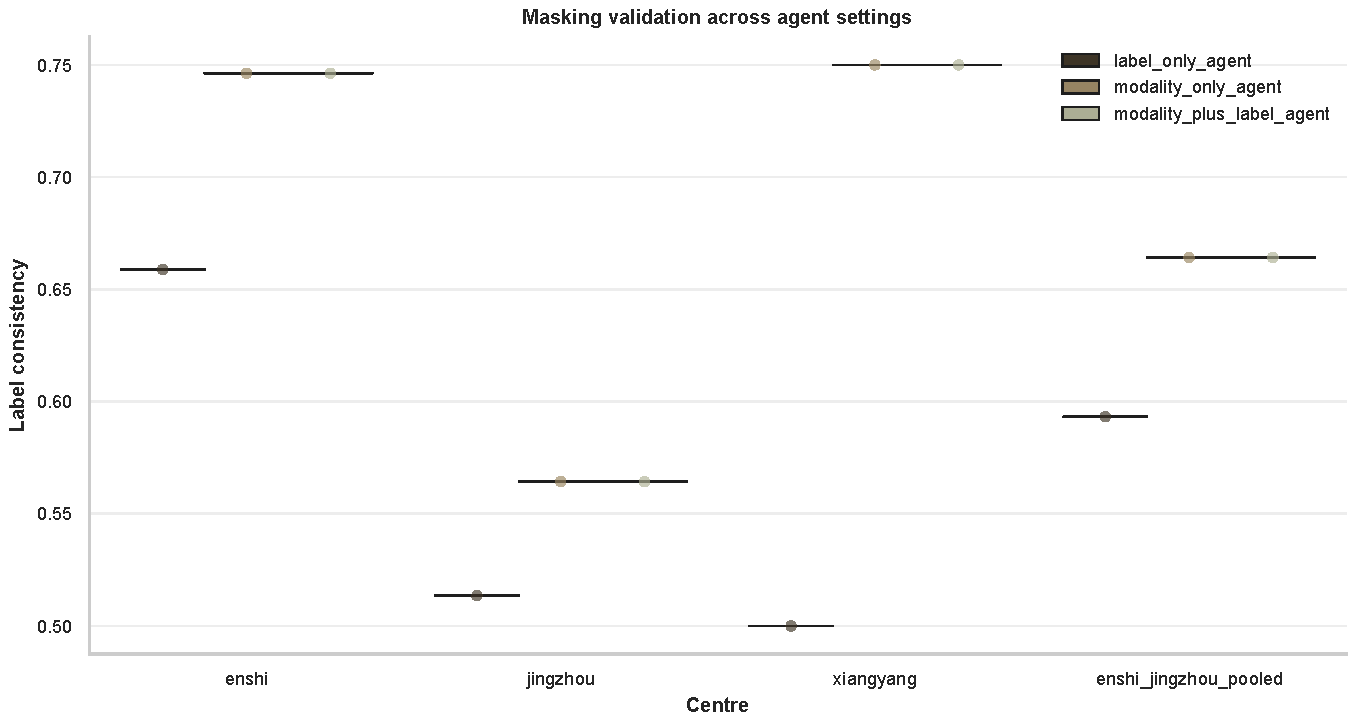
\includegraphics[width=0.92\linewidth]{final_Fig/SupplementaryFigure_S1_masking_validation.pdf}
%   \caption{LCAD masking validation: label-only versus modality-conditioned proxy consistency (Table~S10).}
%   \label{fig:masking_validation}
% \end{figure}

% \subsection{Held-out test performance}
% On the held-out test set ($n=288$), MOSAIC-RASA backbone achieved AUROC 0.832 (95\% CI 0.757--0.897) and F1 0.611 (95\% CI 0.458--0.737) at the validation-selected threshold 0.37.
% Pseudo-augmented (LCAD) training achieved AUROC 0.826 (95\% CI 0.747--0.894) and F1 0.545 at threshold 0.39.
% Real-report-only training yielded AUROC 0.725; simple concatenation fusion yielded AUROC 0.472 (Table~\ref{tab:main_comparison}; Figure~\ref{fig:auc_comparison}).
% Although point estimates were numerically higher for MOSAIC-RASA backbone, paired bootstrap testing did not support a superiority claim ($p\approx 0.5$).

% % >>> 插入位置：Results §3.3 — Table 2 + AUC 图
% \begin{table}[t]
%   \centering
%   \caption{Held-out test performance ($n=288$) at validation-selected thresholds.}
%   \label{tab:main_comparison}
%   \begin{tabular}{lccc}
%     \toprule
%     Model & AUROC [95\% CI] & F1 [95\% CI] & Threshold \\
%     \midrule
%     MOSAIC-RASA backbone        & 0.832 [0.757, 0.897] & 0.611 [0.458, 0.737] & 0.37 \\
%     Pseudo-augmented (LCAD)& 0.826 [0.747, 0.894] & 0.545 [0.395, 0.674] & 0.39 \\
%     Real-report only       & 0.725 [0.640, 0.801] & 0.356 [0.263, 0.438] & 0.14 \\
%     Simple concat fusion   & 0.472 [0.384, 0.563] & 0.265 [0.200, 0.326] & 0.05 \\
%     \bottomrule
%   \end{tabular}
% \end{table}
% >>> 插入位置：Methods 开头或 Introduction 后 — Figure 1 流水线
% \begin{figure}[t]
%   \centering
%   \includegraphics[width=\linewidth]{cervix_lcad_rasa/outputs/publishable/figures/main/Figure1_study_design.pdf}
%   \caption{Overview of the MOSAIC framework under the locked retrospective protocol.}
%   \label{fig:mosaic_overview}
% \end{figure}


% \begin{figure}[t]
%   \centering
%   \includegraphics[width=\linewidth]{final_Fig/Figure_main_AUC_comparison.pdf}
%   \caption{Held-out test AUROC with 95\% bootstrap confidence intervals (Table~\ref{tab:main_comparison}).}
%   \label{fig:auc_comparison}
% \end{figure}

% \subsection{Reference-stratified and cross-centre behaviour}
% Stratified by reference availability, MOSAIC-RASA backbone AUROC was 0.824 ($n=108$ with reference) and 0.850 ($n=180$ without reference).
% Strict LOCO retraining (Table~S2) showed centre-dependent AUROC (Enshi held-out 0.702, Jingzhou 0.648, Xiangyang 0.382 for MOSAIC-RASA backbone).
% Eval-only LOCO (Table~S2b) is reported separately.
% All LOCO models used a fixed quick training budget per fold.

% % >>> 插入位置：Results §3.4 — Figure 4 (optional main) + Table S2
% \begin{figure}[t]
%   \centering
%   \includegraphics[width=\linewidth]{final_Fig/Figure4_loco_strict.pdf}
%   \caption{Strict leave-one-centre-out AUROC under quick-budget retraining (Table~S2).}
%   \label{fig:loco_strict}
% \end{figure}

% \subsection{Ablation studies}
% Modality ablations (Table~S3, nine configurations) ranked input combinations up to AUROC 0.787 (colposcopy+instruction).
% RASA component ablations (Table~S5, seven configurations) showed large degradation without section alignment (AUROC 0.512 versus full 0.806).
% Effects are reported as diagnostic ablations rather than definitive mechanistic proof.

% \subsection{Perturbation fidelity}
% On $n=128$ report-missing test cases (Figure~\ref{fig:perturbation}; Table~S6), normal decoding showed near-unity section similarity.
% Masking OCT reduced \texttt{oct\_findings} similarity to 0.26; masking colposcopy to 0.00; masking instruction reduced \texttt{clinical\_context} to 0.17.
% Label-only inference increased $\Delta$risk by +0.37 versus normal.

% % >>> 插入位置：Results §3.6 — Figure 3 (主文机制图)
% \begin{figure}[t]
%   \centering
%   \includegraphics[width=\linewidth]{final_Fig/Figure3_perturbation.pdf}
%   \caption{Perturbation condition $\times$ report-section similarity ($n=128$).}
%   \label{fig:perturbation}
% \end{figure}

% \subsection{Stability, safety and scalability}
% Multi-seed stability (Table~S7), report-safety indicators (Table~S9), and pipeline scale ($\sim$137k images; checkpoint $\sim$80\,MB; Table~S11) support reproducible big-data batch analytics.

% % >>> 插入位置：Results §3.7 — Supp Fig S3/S4（可选）
% \begin{figure}[t]
%   \centering
%   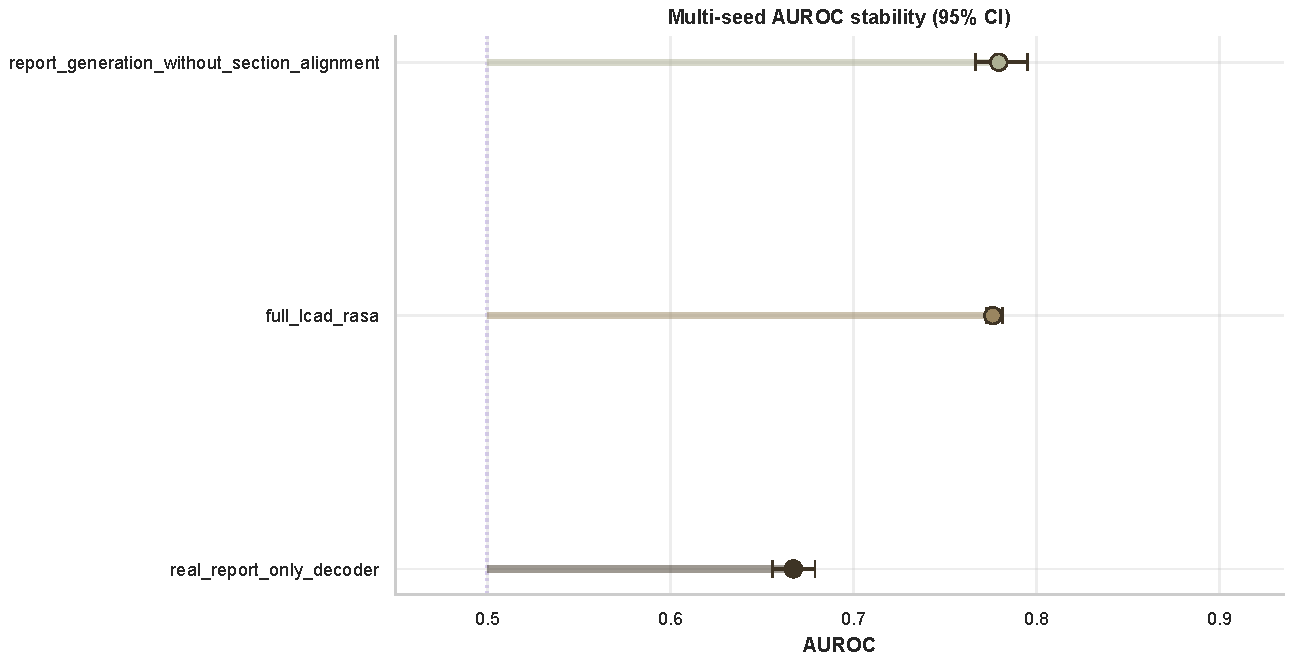
\includegraphics[width=0.48\linewidth]{final_Fig/SupplementaryFigure_S3_multiseed.pdf}
%   \hfill
%   \includegraphics[width=0.48\linewidth]{final_Fig/SupplementaryFigure_S4_scalability.pdf}
%   \caption{Multi-seed stability (left, Table~S7) and scalability summary (right, Table~S11).}
%   \label{fig:stability_scalability}
% \end{figure}

% \subsection{Expert review status}
% An expert-rating template was prepared, but physician scores were not available; physician-validation claims were therefore not made.

% % >>> 插入位置：Methods 开头或 Introduction 后 — Figure 1 流水线
% \begin{figure}[t]
%   \centering
%   \includegraphics[width=\linewidth]{final_Fig/Figure1_study_design.pdf}
%   \caption{Overview of the MOSAIC framework.}
%   \label{fig:mosaic_overview}
% \end{figure}




% \subsection{Implementation, Privacy, and Reproducibility}
% \label{subsec:methods_implementation}

% All analyses were implemented in Python using PyTorch and standard scientific-computing packages. Visual embeddings, structured report schemas, pseudo-report QC outputs, prediction files, manuscript tables, and generated figures were exported as reproducibility artefacts. Random seeds and locked split files were used where applicable.

% External provider comparisons used only de-identified structured evidence. Raw images, raw file paths, patient names, internal patient identifiers, hospital identifiers, phone numbers, identity numbers, and exact clinical record identifiers were not transmitted to external providers.

% This retrospective study does not claim prospective clinical deployment or autonomous decision support. Generated reports were used as weak semantic supervision and audit artefacts; they were not treated as clinical records. Expert physician ratings were not available for the present manuscript version and are therefore not claimed as completed validation. Ethics approval, consent waiver or consent procedure, and institutional review board identifiers should be inserted by the authors according to local requirements.



% \begin{landscape}
% \begin{center}
%   \begin{minipage}{1\linewidth}
%     \captionsetup{type=table}
%     \captionof{table}{Baseline characteristics of the final five-centre multimodal analytic cohort, overall and by participating centre}
%     \label{tab:baseline_all3000_5cens}
%     \normalsize
%     \setlength{\tabcolsep}{2pt}
%     \renewcommand{\arraystretch}{1.8}
%     \begin{adjustbox}{width=\linewidth}
%     \begin{tabular}{c >{\raggedright\arraybackslash}p{4.2cm} c c c c *{12}{c}}
%       \toprule
%       \textbf{No.} & \textbf{Participating centre} & \makecell[c]{\textbf{Archived}\\ \textbf{colposcopy}\\ \textbf{report}} & \makecell[c]{\textbf{Cases with}\\ \textbf{archived report,}\\ \textbf{n (\%)}} & \makecell[c]{\textbf{Examinations,}\\ \textbf{n}} & \makecell[c]{\textbf{Total images,}\\ \textbf{n}} & \makecell[c]{\textbf{Age, years,}\\ \textbf{mean (SD)}} & \makecell[c]{\textbf{hrHPV positive}\\ \textbf{by prespecified}\\ \textbf{genotype panel,}\\ \textbf{n (\%)}} & \makecell[c]{\textbf{HPV status}\\ \textbf{unavailable or}\\ \textbf{unclassifiable,}\\ \textbf{n (\%)}} & \makecell[c]{\textbf{Negative}\\ \textbf{cytology,}\\ \textbf{n (\%)}} & \makecell[c]{\textbf{ASC-US,}\\ \textbf{n (\%)}} & \makecell[c]{\textbf{LSIL or}\\ \textbf{worse,}\\ \textbf{n (\%)}} & \makecell[c]{\textbf{Missing}\\ \textbf{cytology,}\\ \textbf{n (\%)}} & \makecell[c]{\textbf{Positive}\\ \textbf{OCT--clinical}\\ \textbf{training label,}\\ \textbf{n (\%)}} & \makecell[c]{\textbf{CIN0--1 or}\\ \textbf{mapped benign}\\ \textbf{histology,}\\ \textbf{n (\%)}} & \makecell[c]{\textbf{CIN2 or}\\ \textbf{ungraded}\\ \textbf{HSIL,}\\ \textbf{n (\%)}} & \makecell[c]{\textbf{CIN3+,}\\ \textbf{n (\%)}} & \makecell[c]{\textbf{Invasive}\\ \textbf{cervical cancer,}\\ \textbf{n (\%)}} \\
%       \midrule
%       1 & Renmin Hospital of Wuhan University & No & 0 (0.0) & 89 & 10,947 & 45.6 (13.1) & 0 (0.0) & 89 (100.0) & 21 (23.6) & 0 (0.0) & 0 (0.0) & 68 (76.4) & 89 (100.0) & 7 (7.9) & 33 (37.1) & 33 (37.1) & 16 (18.0) \\
%       2 & Enshi Central Hospital & Yes & 406 (100.0) & 406 & 49,737 & 48.8 (11.0) & 20 (4.9) & 386 (95.1) & 88 (21.7) & 20 (4.9) & 13 (3.2) & 285 (70.2) & 131 (32.3) & 276 (68.0) & 66 (16.3) & 45 (11.1) & 19 (4.7) \\
%       3 & Xiangyang Central Hospital & Sparse & 4 (0.8) & 500 & 45,757 & 45.9 (10.2) & 74 (14.8) & 426 (85.2) & 75 (15.0) & 60 (12.0) & 56 (11.2) & 309 (61.8) & 80 (16.0) & 392 (78.4) & 47 (9.4) & 27 (5.4) & 34 (6.8) \\
%       4 & Shiyan People's Hospital & No & 0 (0.0) & 496 & 15,755 & 41.8 (11.3) & 160 (32.3) & 336 (67.7) & 60 (12.1) & 73 (14.7) & 57 (11.5) & 306 (61.7) & 35 (7.1) & 479 (96.6) & 13 (2.6) & 0 (0.0) & 4 (0.8) \\
%       5 & Jingzhou First People's Hospital & Yes & 334 (82.3) & 406 & 15,395 & 47.0 (11.4) & 183 (45.1) & 223 (54.9) & 50 (12.3) & 118 (29.1) & 33 (8.1) & 205 (50.5) & 38 (9.4) & 369 (90.9) & 24 (5.9) & 3 (0.7) & 10 (2.5) \\
%       \rowcolor{gray!10}
%        & Overall & Partial & 744 (39.2) & 1897 & 137,591 & 45.7 (11.4) & 437 (23.0) & 1460 (77.0) & 294 (15.5) & 271 (14.3) & 159 (8.4) & 1173 (61.8) & 373 (19.7) & 1523 (80.3) & 183 (9.6) & 108 (5.7) & 83 (4.4) \\
%       \bottomrule
%     \end{tabular}
%     \end{adjustbox}
%     \vspace{0.4em}
%     \begin{minipage}{\linewidth}
%       \footnotesize
%       \textit{The final analytic cohort comprised examinations with paired OCT volumes, colposcopy still images, and clinical priors linked to administrative registry records. The registry included 3,010 screened examinations and 3,009 unique OCT identifiers after de-duplication, from which a final multimodal cohort of 1,897 examinations with verified imaging was derived. Images denote the total number of OCT B-scan image files plus colposcopy still-image files available for the final analytic cohort; archived report images, Report.ini files, and pixel-guidance masks were not counted. Archived colposcopy-report availability describes the source archives only and was not used as a model input. Centres classified as ``Yes'' had structured report exports available (e.g., report images from Jingzhou and PDF/XML records from Enshi). Wuhan and Shiyan archives contained only colposcopy images, whereas Xiangyang had sparse report availability. ``Cases with archived report'' denotes examinations for which at least one structured report file was present in the clinical archive. hrHPV positivity was defined according to the prespecified high-risk genotype panel: HPV 16, 18, 31, 33, 35, 39, 45, 51, 52, 53, 56, 58, 59, 66, 68, 73, 81, oHmyr 82. The positive OCT--clinical training label denotes the harmonised binary supervision label used for multimodal model training and was derived from OCT second-read text when definitive pathology mapping was unavailable. CIN categories were harmonised from clinical pathology reports and downstream treatment or excision records when available. Ungraded high-grade CIN or HSIL without explicit CIN3 or AIS terminology was conservatively assigned to the CIN2/HSIL category; explicit CIN2--3 was classified as CIN3+. Invasive cervical cancer required explicit invasive-cancer terminology in a cervical context or corroborating downstream excision records.}
%     \end{minipage}
%   \end{minipage}
% \end{center}
% \end{landscape}



\section{Experiments and Results}
\label{sec:experiments_results}

The experimental evaluation was designed to test MOSAIC as a multimodal learning framework under imbalanced report supervision. We first describe the five-centre data setting, the locked train/validation/test protocol, and the report-availability bottleneck that motivates weak-oracle learning. We then evaluate predictive performance against same-split baselines, quantify the contribution of the main MOSAIC components through ablation studies, and examine whether the retrieval-calibrated gain depends on report-derived semantic priors rather than uncontrolled leakage. Additional analyses assess report-scarcity behaviour, section-level alignment, parameter and mechanism sensitivity, perturbation robustness, centre-shift stress, and computational efficiency. This organisation separates the primary performance evidence from auxiliary audits and keeps the interpretation bounded: MOSAIC is evaluated as a retrospective, leakage-controlled analytics framework for report-imbalanced multimodal data, not as a prospectively validated clinical device.

\clearpage
\begin{landscape}
\begin{table}[p]
  \centering
  \caption{Experimental questions and evidence structure.}
  \label{tab:rq_evidence_map}
  \scriptsize
  \setlength{\tabcolsep}{4pt}
  \renewcommand{\arraystretch}{1.35}
  \begin{threeparttable}
  \resizebox{\linewidth}{!}{%
  \begin{tabular}{p{3.0cm}p{4.8cm}p{5.8cm}p{5.8cm}p{5.4cm}}
    \toprule
    \textbf{Evaluation axis} & \textbf{Main question} & \textbf{Primary evidence} & \textbf{Secondary audit or sensitivity evidence} & \textbf{Claim boundary} \\
    \midrule
    Data setting and protocol
    & What supervision imbalance defines the learning problem, and how is leakage controlled?
    & Five-centre cohort description, locked train/validation/test split, report-availability distribution, and centre-stratified supervision map
    & Case-level split audit, report-availability stratification, and exclusion of validation/test labels from pseudo-report generation, bank construction, fusion calibration, and threshold selection
    & The cohort supports retrospective multimodal analytics under incomplete report supervision; it is not a prospective clinical validation cohort. \\
    \addlinespace[2pt]
    Baseline performance
    & Does MOSAIC improve locked held-out prediction against same-split multimodal baselines?
    & Held-out AUROC, AUPRC, F1, sensitivity, precision, balanced accuracy, and paired-bootstrap comparisons with clinical, single-modality, late-fusion, cross-attention, and CLIP-style baselines
    & Score-separation analysis, centre-wise gain profiles, and paired uncertainty estimates using case-id-aligned predictions
    & Superiority over the MOSAIC-RASA backbone is tested; comparison with the strongest contrastive baseline is interpreted as competitive rather than conclusive. \\
    \addlinespace[2pt]
    Module contribution
    & Which components account for the observed behaviour?
    & Pseudo-report source comparison, report-scarcity ablation, RASA modality-section retrieval, retrieval-only prior, and full retrieval-calibrated fusion
    & Semantic-tag controls, negative controls, no-section ablation, simple-fusion ablation, and QC failure-enriched stress testing
    & Generated reports are used as bounded weak semantic supervision. They do not replace clinician-authored reports or pathology-derived/harmonised endpoints. \\
    \addlinespace[2pt]
    Parameter and mechanism sensitivity
    & Are the alignment and retrieval mechanisms stable under key design choices?
    & Alignment-weight sweep, modality ablations, component ablations, train-only retrieval fusion, and validation-locked threshold analysis
    & Perturbation analysis for OCT, colposcopy, clinical instruction, visual masking, and label-only inference
    & Section alignment is interpreted as relative semantic organisation and modality responsiveness, not causal identification or high-fidelity semantic retrieval. \\
    \addlinespace[2pt]
    Robustness, centre shift, and efficiency
    & Where does the framework remain informative, and where should its claims stop?
    & CIN3+ proxy safety-oriented audit, semantic-tag leakage audit, strict leave-one-centre-out stress test, and scale/storage analysis
    & Reference-stratified testing, same-centre-excluded retrieval, random query controls, random label-bank controls, and embedding/path leakage checks
    & The evidence supports a retrospective, leakage-controlled analytics framework. It does not establish prospective deployment, centre-invariant generalisation, autonomous LLM decision-making, or unrestricted clinical safety. \\
    \bottomrule
  \end{tabular}%
  }
  % \begin{tablenotes}[flushleft]
  %   \footnotesize
  %   \item This table is intentionally placed as a landscape full-page evidence map because it defines the structure of the experimental section. The detailed numerical results are reported in the corresponding subsections.
  % \end{tablenotes}
  \end{threeparttable}
\end{table}
\end{landscape}
\clearpage

\FloatBarrier

\subsection{Experimental Setting and Report-Supervision Imbalance}
\label{subsec:cohort_results}

The final analytic cohort contained 1,897 multimodal cervical screening cases from five centres. Each case had paired OCT volumes, colposcopy image files, and structured clinical variables, including HPV, TCT, and age fields where available. The cohort contained 137,591 evaluable OCT and colposcopy-associated image files. Clinician-authored report supervision was much less complete: archived reports were available for 744 cases, while 1,153 cases had multimodal evidence but no archived report. Table~\ref{tab:baseline_all3000_5cens} provides a compact cohort summary, and Figure~\ref{fig:centre_supervision} visualises the centre-level imbalance.

\begin{landscape}
\begin{center}
  \begin{minipage}{1\linewidth}
    \captionsetup{type=table}
    \captionof{table}{Baseline characteristics of the final five-centre multimodal analytic cohort, overall and by participating centre}
    \label{tab:baseline_all3000_5cens}
    \normalsize
    \setlength{\tabcolsep}{2pt}
    \renewcommand{\arraystretch}{1.8}
    \begin{adjustbox}{width=\linewidth}
    \begin{tabular}{c >{\raggedright\arraybackslash}p{4.2cm} c c c c *{12}{c}}
      \toprule
      \textbf{No.} & \textbf{Participating centre} & \makecell[c]{\textbf{Archived}\\ \textbf{colposcopy}\\ \textbf{report}} & \makecell[c]{\textbf{Cases with}\\ \textbf{archived report,}\\ \textbf{n (\%)}} & \makecell[c]{\textbf{Examinations,}\\ \textbf{n}} & \makecell[c]{\textbf{Total images,}\\ \textbf{n}} & \makecell[c]{\textbf{Age, years,}\\ \textbf{mean (SD)}} & \makecell[c]{\textbf{hrHPV positive}\\ \textbf{by prespecified}\\ \textbf{genotype panel,}\\ \textbf{n (\%)}} & \makecell[c]{\textbf{HPV status}\\ \textbf{unavailable or}\\ \textbf{unclassifiable,}\\ \textbf{n (\%)}} & \makecell[c]{\textbf{Negative}\\ \textbf{cytology,}\\ \textbf{n (\%)}} & \makecell[c]{\textbf{ASC-US,}\\ \textbf{n (\%)}} & \makecell[c]{\textbf{LSIL or}\\ \textbf{worse,}\\ \textbf{n (\%)}} & \makecell[c]{\textbf{Missing}\\ \textbf{cytology,}\\ \textbf{n (\%)}} & \makecell[c]{\textbf{Positive}\\ \textbf{OCT--clinical}\\ \textbf{training label,}\\ \textbf{n (\%)}} & \makecell[c]{\textbf{CIN0--1 or}\\ \textbf{mapped benign}\\ \textbf{histology,}\\ \textbf{n (\%)}} & \makecell[c]{\textbf{CIN2 or}\\ \textbf{ungraded}\\ \textbf{HSIL,}\\ \textbf{n (\%)}} & \makecell[c]{\textbf{CIN3+,}\\ \textbf{n (\%)}} & \makecell[c]{\textbf{Invasive}\\ \textbf{cervical cancer,}\\ \textbf{n (\%)}} \\
      \midrule
      1 & Renmin Hospital of Wuhan University & No & 0 (0.0) & 89 & 10,947 & 45.6 (13.1) & 0 (0.0) & 89 (100.0) & 21 (23.6) & 0 (0.0) & 0 (0.0) & 68 (76.4) & 89 (100.0) & 7 (7.9) & 33 (37.1) & 33 (37.1) & 16 (18.0) \\
      2 & Enshi Central Hospital & Yes & 406 (100.0) & 406 & 49,737 & 48.8 (11.0) & 20 (4.9) & 386 (95.1) & 88 (21.7) & 20 (4.9) & 13 (3.2) & 285 (70.2) & 131 (32.3) & 276 (68.0) & 66 (16.3) & 45 (11.1) & 19 (4.7) \\
      3 & Xiangyang Central Hospital & Sparse & 4 (0.8) & 500 & 45,757 & 45.9 (10.2) & 74 (14.8) & 426 (85.2) & 75 (15.0) & 60 (12.0) & 56 (11.2) & 309 (61.8) & 80 (16.0) & 392 (78.4) & 47 (9.4) & 27 (5.4) & 34 (6.8) \\
      4 & Shiyan People's Hospital & No & 0 (0.0) & 496 & 15,755 & 41.8 (11.3) & 160 (32.3) & 336 (67.7) & 60 (12.1) & 73 (14.7) & 57 (11.5) & 306 (61.7) & 35 (7.1) & 479 (96.6) & 13 (2.6) & 0 (0.0) & 4 (0.8) \\
      5 & Jingzhou First People's Hospital & Yes & 334 (82.3) & 406 & 15,395 & 47.0 (11.4) & 183 (45.1) & 223 (54.9) & 50 (12.3) & 118 (29.1) & 33 (8.1) & 205 (50.5) & 38 (9.4) & 369 (90.9) & 24 (5.9) & 3 (0.7) & 10 (2.5) \\
      \rowcolor{gray!10}
       & Overall & Partial & 744 (39.2) & 1897 & 137,591 & 45.7 (11.4) & 437 (23.0) & 1460 (77.0) & 294 (15.5) & 271 (14.3) & 159 (8.4) & 1173 (61.8) & 373 (19.7) & 1523 (80.3) & 183 (9.6) & 108 (5.7) & 83 (4.4) \\
      \bottomrule
    \end{tabular}
    \end{adjustbox}
    \vspace{0.4em}
    \begin{minipage}{\linewidth}
      \footnotesize
      \textit{The final analytic cohort comprised examinations with paired OCT volumes, colposcopy image files, and clinical priors linked to administrative registry records. The registry included 3,010 screened examinations and 3,009 unique OCT identifiers after de-duplication, from which a final multimodal cohort of 1,897 examinations with verified imaging was derived. Image counts were recomputed from the canonical case manifest and denote the image files recorded in the OCT and colposcopy path fields for the final analytic cohort (129,030 OCT files and 8,561 colposcopy-associated files). Archived colposcopy-report availability describes the source archives only and was not used as a model input. Centres classified as ``Yes'' had structured report exports available (e.g., report images from Jingzhou and PDF/XML records from Enshi). Wuhan and Shiyan archives contained only colposcopy images, whereas Xiangyang had sparse report availability. ``Cases with archived report'' denotes examinations for which at least one structured report file was present in the clinical archive. hrHPV positivity was defined according to the prespecified high-risk genotype panel: HPV 16, 18, 31, 33, 35, 39, 45, 51, 52, 53, 56, 58, 59, 66, 68, 73, 81, oHmyr 82. The positive OCT--clinical training label denotes the harmonised binary supervision label used for multimodal model training and was derived from OCT second-read text when definitive pathology mapping was unavailable. CIN categories were harmonised from clinical pathology reports and downstream treatment or excision records when available. Ungraded high-grade CIN or HSIL without explicit CIN3 or AIS terminology was conservatively assigned to the CIN2/HSIL category; explicit CIN2--3 was classified as CIN3+. Invasive cervical cancer required explicit invasive-cancer terminology in a cervical context or corroborating downstream excision records.}
    \end{minipage}
  \end{minipage}
\end{center}
\end{landscape}

The missingness pattern was strongly centre-dependent. Enshi retained reports for all 406 cases, Jingzhou retained reports for 334 of 406 cases, Xiangyang retained reports for only 4 of 500 cases, and Wuhan and Shiyan had no centre-wide report archive. The central data problem was therefore not image acquisition. It was the uneven availability of report-level semantic supervision. This pattern motivates the weak-oracle formulation: real reports are preserved when available, while report-missing cases are allowed to contribute only through structured, QC-gated, and auditable semantic supervision.

\begin{figure}[!htbp]
  \centering
  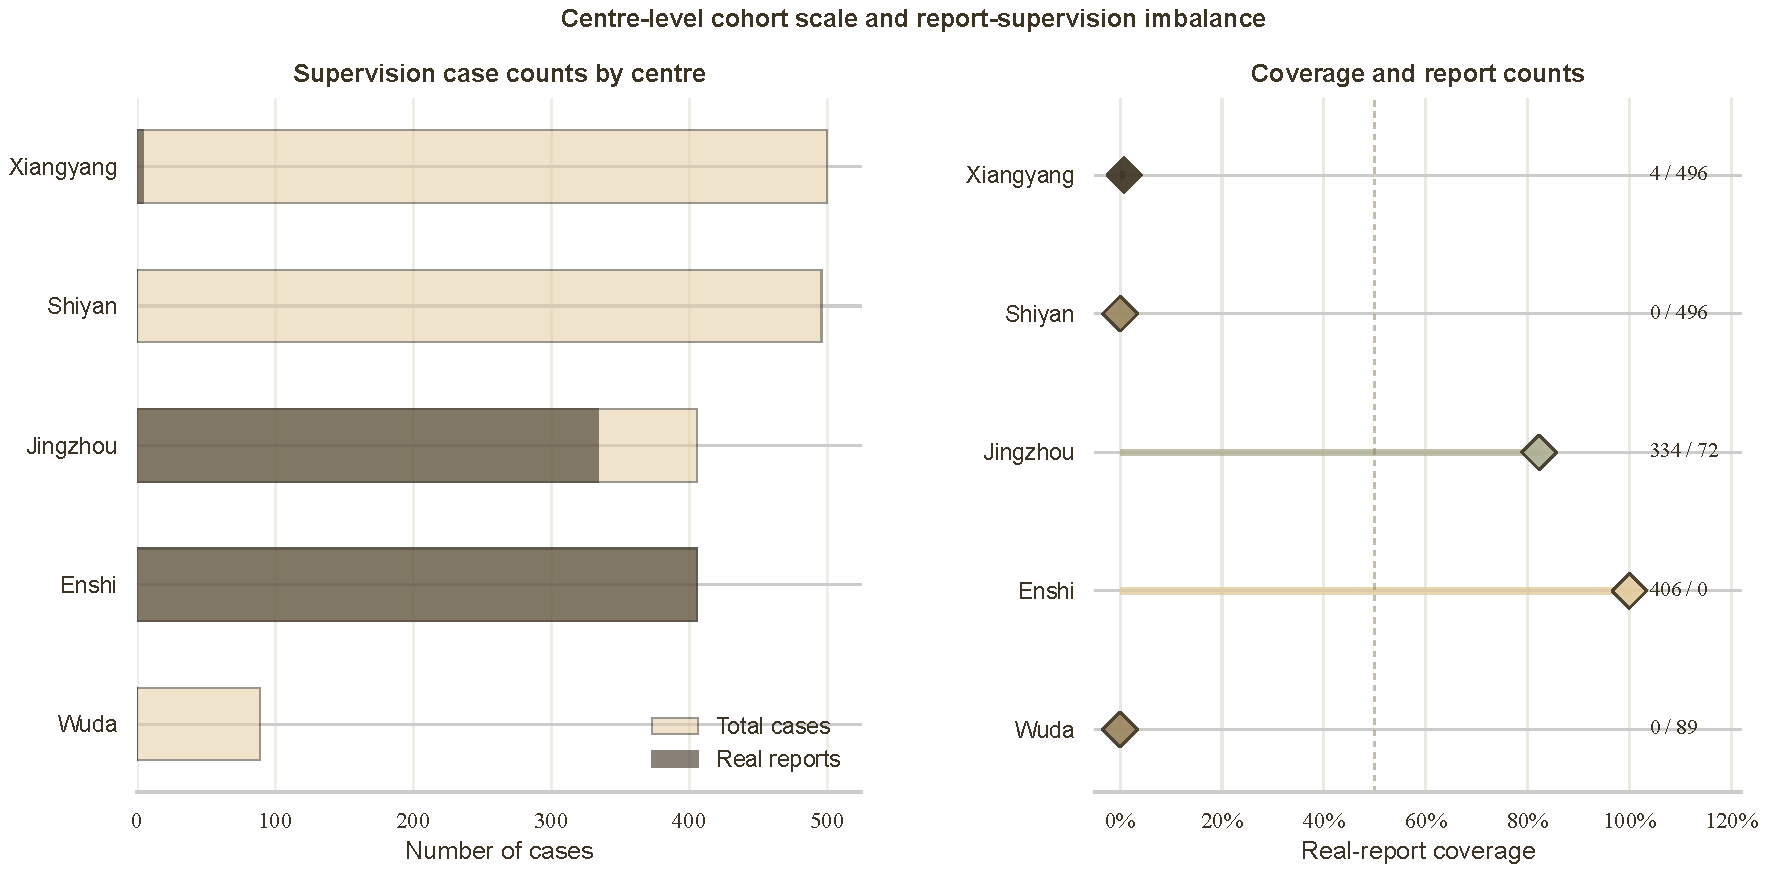
\includegraphics[width=\linewidth]{final_Fig/Figure2_centre_supervision_catplot.pdf}
  \caption{Centre-stratified cohort scale and report-supervision availability. The plot summarises case counts, image volume, and report coverage across centres. It highlights the mismatch between large-scale multimodal evidence and uneven clinician-authored report supervision.}
  \label{fig:centre_supervision}
\end{figure}

\FloatBarrier

\subsection{Main Performance and Same-Split Baseline Comparison}
\label{subsec:mosaic_main_results}

The primary performance experiment evaluated whether report-derived semantic priors improve held-out prediction under a locked protocol. The semantic memory bank was built from the training split only. The fusion weight was selected on the validation split only and then locked for test evaluation. The held-out test set contained 288 cases.

MOSAIC-RASA, the backbone before retrieval calibration, achieved AUROC 0.856, AUPRC 0.662, and F1 0.519. The semantic retrieval prior alone achieved AUROC 0.774, AUPRC 0.589, and F1 0.585, indicating useful but insufficient standalone signal. After validation-calibrated logit fusion with \(\alpha=0.31\) and threshold \(0.50\), MOSAIC reached AUROC 0.908, AUPRC 0.741, and F1 0.736. Sensitivity was 0.727, precision was 0.744, and balanced accuracy was 0.841 (Table~\ref{tab:mosaic_main}).

\begin{table*}[!htbp]
  \centering
  \caption{Locked held-out test performance of MOSAIC and its retrieval components ($n=288$).}
  \label{tab:mosaic_main}
  \scriptsize
  \begin{threeparttable}
  \resizebox{\linewidth}{!}{%
  \begin{tabular}{lrrrrrrr}
    \toprule
    \textbf{Method} & \textbf{AUROC} & \textbf{AUPRC} & \textbf{F1} & \textbf{Sensitivity} & \textbf{Precision} & \textbf{Balanced acc.} & \textbf{Threshold} \\
    \midrule
    MOSAIC-RASA backbone & 0.856 & 0.662 & 0.519 & 0.636 & 0.438 & 0.744 & 0.39 \\
    Semantic retrieval only & 0.774 & 0.589 & 0.585 & 0.545 & 0.632 & 0.744 & 0.67 \\
    \textbf{MOSAIC} & \textbf{0.908} & \textbf{0.741} & \textbf{0.736} & \textbf{0.727} & \textbf{0.744} & \textbf{0.841} & 0.50 \\
    \midrule
    \multicolumn{8}{l}{MOSAIC vs MOSAIC-RASA backbone: \(\Delta\)AUROC 0.053; 95\% paired bootstrap CI 0.012--0.101; two-sided \(p=0.005\) (2,000 resamples).} \\
    \bottomrule
  \end{tabular}%
  }
  \begin{tablenotes}[flushleft]
    \footnotesize
    \item The semantic retrieval bank was built from training cases only. The fusion weight \(\alpha=0.31\) and operating threshold \(0.50\) were selected on validation data and locked before test evaluation.
  \end{tablenotes}
  \end{threeparttable}
\end{table*}

\begin{figure}[!htbp]
  \centering
  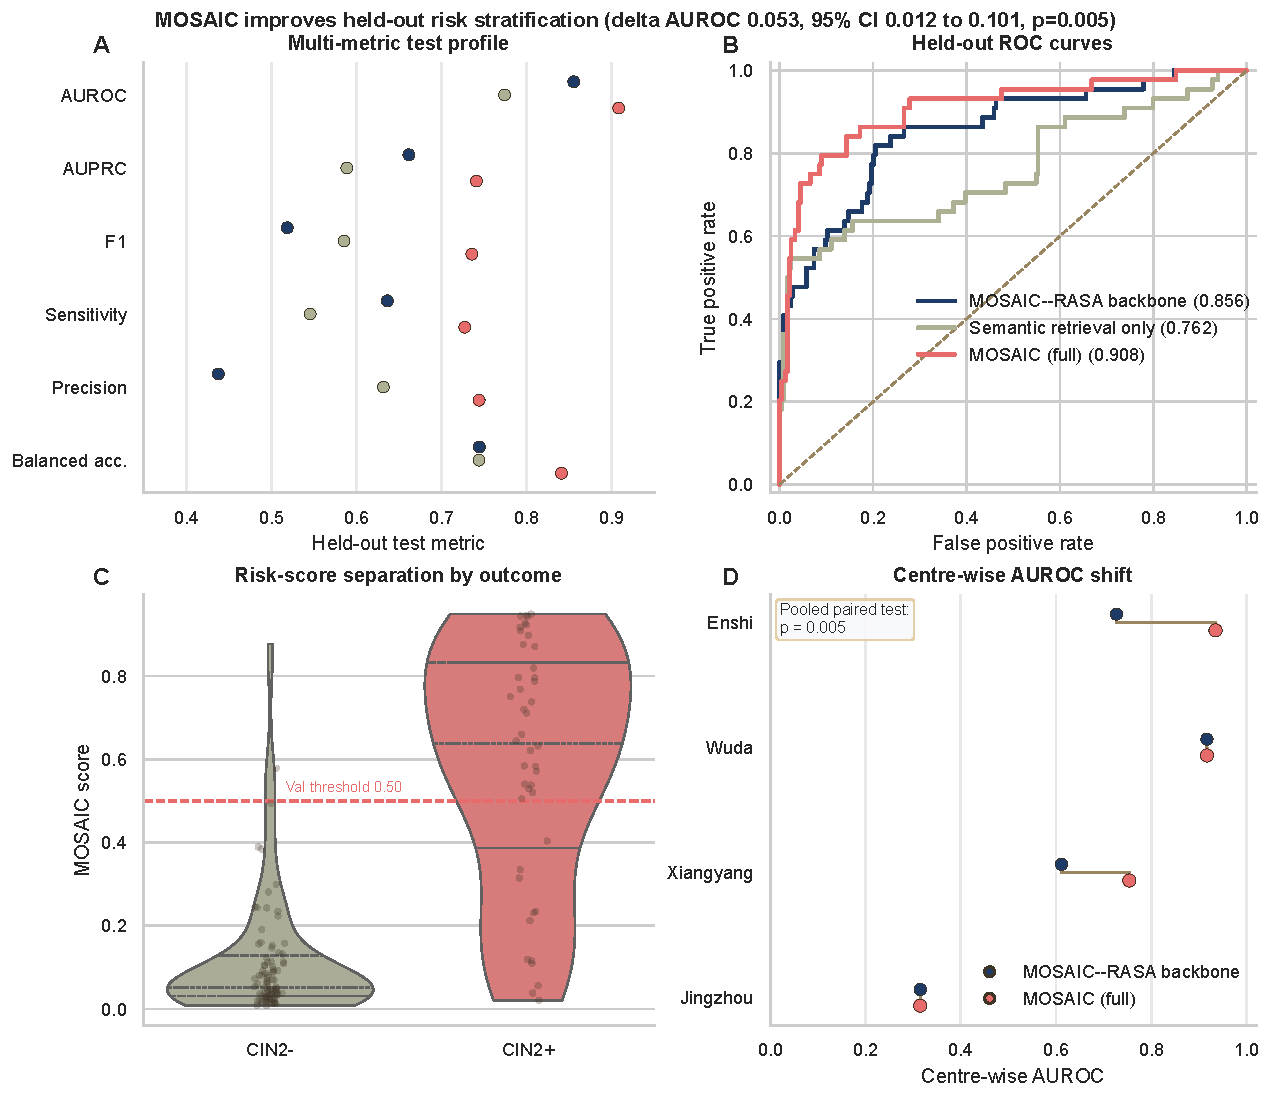
\includegraphics[width=\linewidth]{final_Fig/Figure_mosaic_performance_summary.pdf}
  \caption{Held-out risk stratification by MOSAIC. The panels summarise test-set metrics, ROC curves, score separation by outcome, and centre-wise AUROC shifts relative to the MOSAIC-RASA backbone. The primary paired estimate is \(\Delta\)AUROC 0.053 with 95\% CI 0.012--0.101 and two-sided \(p=0.005\), as reported in Table~\ref{tab:mosaic_main}.}
  \label{fig:mosaic_performance_summary}
\end{figure}
% If the embedded title inside Figure_mosaic_performance_summary.pdf still contains legacy values, regenerate the source figure so that the displayed CI and p-value match Table~\ref{tab:mosaic_main}.

The improvement over the backbone was statistically supported by the paired bootstrap audit. Historical pre-retrieval backbone values, including the 0.832 AUROC internal block, are retained only as protocol-harmonisation evidence and are not used as the primary result. A neural token-packer checkpoint also did not improve the stable-hash backbone on its own (0.853 versus 0.856). It is therefore treated as an exploratory ablation rather than as part of the MOSAIC definition.

\subsubsection{Comparison with External Baselines}
\label{subsec:external_baseline_results}

The same-split baseline study tested whether MOSAIC remained competitive against standard discriminative multimodal models. All baselines used the same train/validation/test split, validation-selected threshold rule, locked held-out test set, and bootstrap protocol. The suite included clinical-only logistic regression, clinical-only HistGradientBoosting, OCT-only and colposcopy-only embedding MLPs, late-fusion MLP, a cross-attention multimodal transformer, and a CLIP-style contrastive multimodal baseline without report-section supervision.

Table~\ref{tab:external_baselines} shows the held-out comparison. MOSAIC achieved the highest AUROC point estimate. The strongest non-MOSAIC comparator was the CLIP-style contrastive baseline, with AUROC 0.888 and F1 0.640. The MOSAIC-RASA backbone alone was comparable to several conventional baselines, but the retrieval-calibrated MOSAIC model was the main method-level comparison.

\begin{table*}[!htbp]
  \centering
  \caption{Same-split comparison of MOSAIC, the MOSAIC-RASA backbone, and external baselines on the locked held-out test set.}
  \label{tab:external_baselines}
  \scriptsize
  \begin{threeparttable}
  \resizebox{\linewidth}{!}{%
  \begin{tabular}{lrrr}
    \toprule
    \textbf{Model} & \textbf{AUROC [95\% CI]} & \textbf{F1 [95\% CI]} & \textbf{Threshold} \\
    \midrule
    \textbf{MOSAIC}                              & \textbf{0.908} [0.845, 0.957] & \textbf{0.736} [0.620, 0.830] & 0.50 \\
    CLIP-style contrastive multimodal baseline  & \underline{0.888} [0.821, 0.942] & \underline{0.640} [0.500, 0.753] & 0.79 \\
    Clinical-only HistGradientBoosting          & 0.862 [0.798, 0.918] & 0.632 [0.507, 0.741] & 0.68 \\
    MOSAIC-RASA backbone (stable-hash)          & 0.856 [0.782, 0.915] & 0.519 [0.411, 0.667] & 0.39 \\
    Cross-attention multimodal transformer      & 0.847 [0.776, 0.908] & 0.522 [0.385, 0.636] & 0.65 \\
    Clinical-only logistic regression           & 0.830 [0.760, 0.889] & 0.557 [0.430, 0.673] & 0.63 \\
    Colposcopy-only embedding MLP               & 0.827 [0.756, 0.890] & 0.510 [0.381, 0.627] & 0.74 \\
    Late-fusion MLP                             & 0.824 [0.750, 0.891] & 0.486 [0.333, 0.625] & 0.77 \\
    OCT-only embedding MLP                      & 0.786 [0.708, 0.861] & 0.494 [0.344, 0.622] & 0.68 \\
    \bottomrule
  \end{tabular}%
  }
  \begin{tablenotes}[flushleft]
    \footnotesize
    \item All rows used the same locked split, validation max-F1 threshold selection, and bootstrap confidence-interval protocol. The stable-hash MOSAIC-RASA backbone is the backbone used for semantic fusion.
  \end{tablenotes}
  \end{threeparttable}
\end{table*}

\begin{figure}[!htbp]
  \centering
  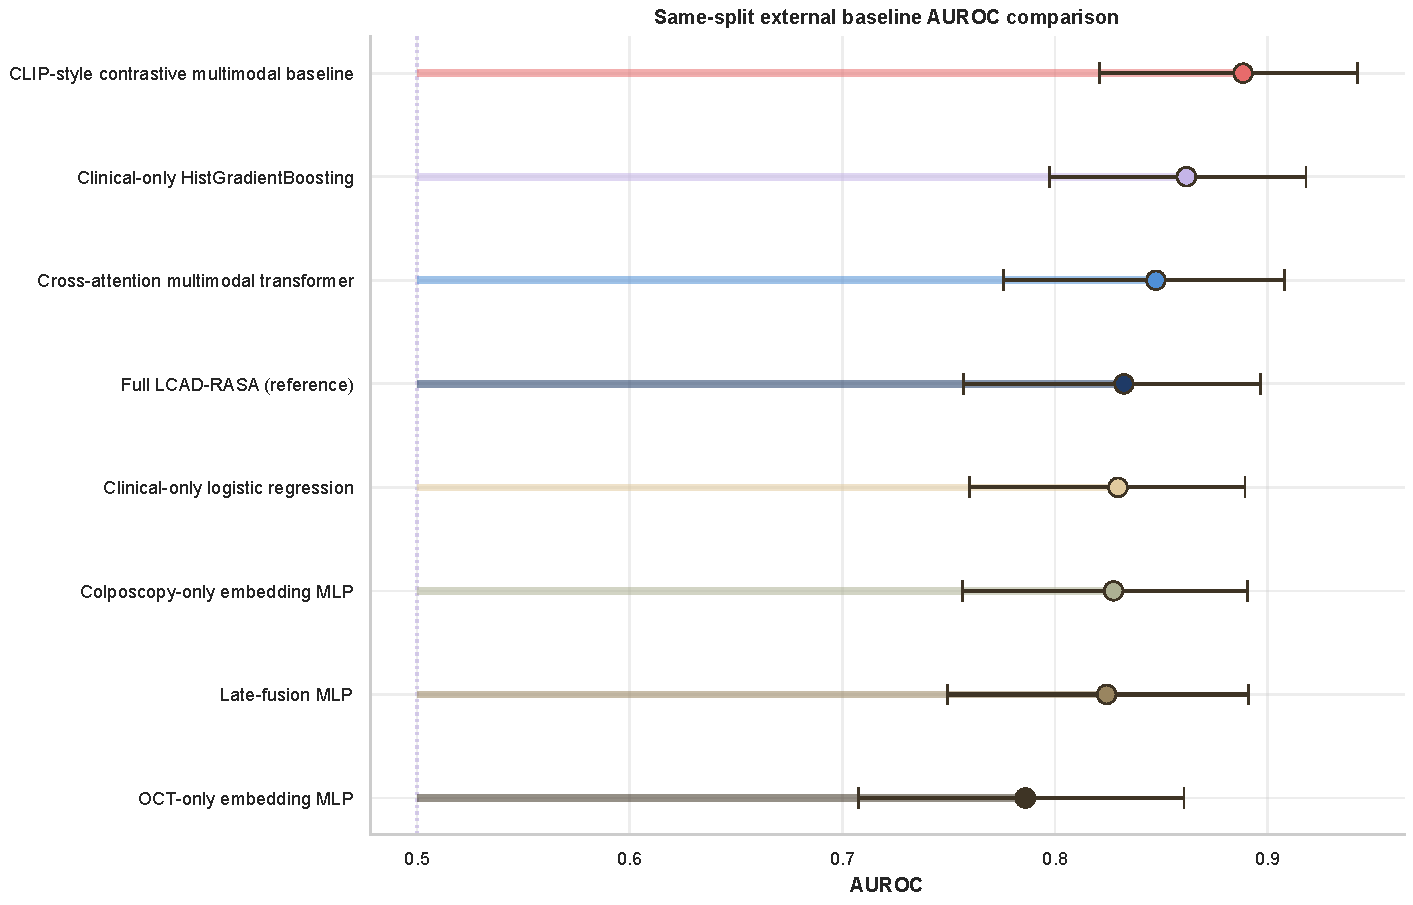
\includegraphics[width=\linewidth]{final_Fig/Figure_external_baselines_auc_forest.pdf}
  \caption{Same-split AUROC comparison among MOSAIC, the stable-hash MOSAIC-RASA backbone, and external baselines. Intervals denote bootstrap 95\% confidence intervals.}
  \label{fig:external_baselines_auc}
\end{figure}
% Ensure that Figure_external_baselines_auc_forest.pdf includes MOSAIC (0.908) and MOSAIC-RASA backbone (0.856). Legacy values such as 0.832 should not appear in this primary comparison figure unless explicitly labelled as legacy.

Paired bootstrap testing further clarifies the comparison (Table~\ref{tab:full_mosaic_paired_bootstrap}). MOSAIC significantly exceeded the MOSAIC-RASA backbone, cross-attention transformer, clinical logistic regression, late-fusion MLP, colposcopy-only MLP, and OCT-only MLP. The comparison with the CLIP-style contrastive baseline was more cautious. MOSAIC had a higher AUROC point estimate (0.908 versus 0.888), but the paired interval crossed zero. This result supports competitiveness and auditability rather than conclusive superiority over the strongest contrastive baseline.

\begin{table*}[!htbp]
  \centering
  \caption{Paired-bootstrap comparison of MOSAIC with same-split baselines. Positive values favour MOSAIC.}
  \label{tab:full_mosaic_paired_bootstrap}
  \scriptsize
  \begin{threeparttable}
  \resizebox{\linewidth}{!}{%
  \begin{tabular}{lrrrrrr}
    \toprule
    \textbf{Comparator} & \textbf{Comparator AUROC} & \textbf{\(\Delta\)AUROC} & \textbf{95\% interval} & \textbf{Two-sided \(p\)} & \textbf{\(\Delta\)AUPRC} & \textbf{\(\Delta\)F1} \\
    \midrule
    CLIP-style contrastive multimodal baseline & 0.888 & 0.020 & [-0.019, 0.065] & 0.355 & 0.002 & 0.096 \\
    Clinical-only HistGradientBoosting         & 0.862 & 0.047 & [-0.015, 0.111] & 0.151 & 0.196 & 0.104 \\
    MOSAIC-RASA backbone                       & 0.856 & 0.053 & [0.012, 0.101] & \textbf{0.005} & 0.079 & 0.217 \\
    Cross-attention multimodal transformer     & 0.847 & 0.061 & [0.013, 0.113] & \textbf{0.011} & 0.107 & 0.214 \\
    Clinical-only logistic regression          & 0.830 & 0.079 & [0.026, 0.136] & \textbf{0.003} & 0.261 & 0.179 \\
    Colposcopy-only embedding MLP              & 0.827 & 0.081 & [0.028, 0.142] & \textbf{0.002} & 0.151 & 0.225 \\
    Late-fusion MLP                            & 0.824 & 0.084 & [0.028, 0.145] & \textbf{0.002} & 0.161 & 0.250 \\
    OCT-only embedding MLP                     & 0.786 & 0.122 & [0.052, 0.197] & \textbf{\(<0.001\)} & 0.194 & 0.242 \\
    \bottomrule
  \end{tabular}%
  }
  \begin{tablenotes}[flushleft]
    \footnotesize
    \item All comparisons used case-id-aligned held-out predictions, 2,000 bootstrap resamples, and locked validation-selected thresholds. Statistically significant \(p\)-values (\(\leq 0.05\)) are highlighted in \textbf{bold}.
  \end{tablenotes}
  \end{threeparttable}
\end{table*}

A generic retrieval-fusion control for every non-MOSAIC baseline was considered but not executed. The available external-baseline files contained locked test predictions but did not include the corresponding validation predictions. Calibrating a retrieval-fusion weight from those files would therefore require tuning on the test set and would violate the locked protocol. This unexecuted control is treated as a limitation rather than as a negative result. A non-report retrieval control using the same train-only neighbourhood mechanism without report-section semantics should be evaluated in future work to further separate semantic-prior effects from generic train-neighbour label memory.

\FloatBarrier

\subsection{Ablation Analysis of Weak-Oracle Completion}
\label{subsec:pseudo_report_results}

The first ablation block tested whether pseudo reports provided modality-grounded supervision or merely converted weak labels into text. Table~\ref{tab:pseudo_source_comparison} and Figure~\ref{fig:pseudo_source_comparison} compare three structured pseudo-report sources. The label-template control was schema-complete, but it had no modality support and showed high repetition, with a maximum duplicate fraction of 0.867. This is a useful negative control. A complete report schema alone does not create useful supervision if the generated sections do not reflect OCT, colposcopy, or clinical evidence.

\begin{table*}[!htbp]
  \centering
  \caption{Structured pseudo-report source comparison under the retrospective protocol.}
  \label{tab:pseudo_source_comparison}
  \scriptsize
  \begin{threeparttable}
  \resizebox{\linewidth}{!}{%
  \begin{tabular}{lrrrrr}
    \toprule
    \textbf{Source} & \textbf{\(n\)} & \textbf{Label consistency} & \textbf{Modality support} & \textbf{Unique text} & \textbf{Duplicate fraction} \\
    \midrule
    Label template                      & 180 & 0.567 & 0.000 & 0.011 & 0.867 \\
    Rule-based                          & 180 & \textbf{0.628} & \textbf{1.000} & \textbf{0.194} & \textbf{0.200} \\
    Local embedding-assisted generator  & 180 & \textbf{0.628} & \textbf{1.000} & \underline{0.156} & \underline{0.261} \\
    \bottomrule
  \end{tabular}%
  }
  \begin{tablenotes}[flushleft]
    \footnotesize
    \item Best results are highlighted in \textbf{bold}, and second-best results are \underline{underlined}. All three sources produced schema-complete reports, so the non-informative complete-rate column was omitted.
  \end{tablenotes}
  \end{threeparttable}
\end{table*}

\begin{figure}[!htbp]
  \centering
  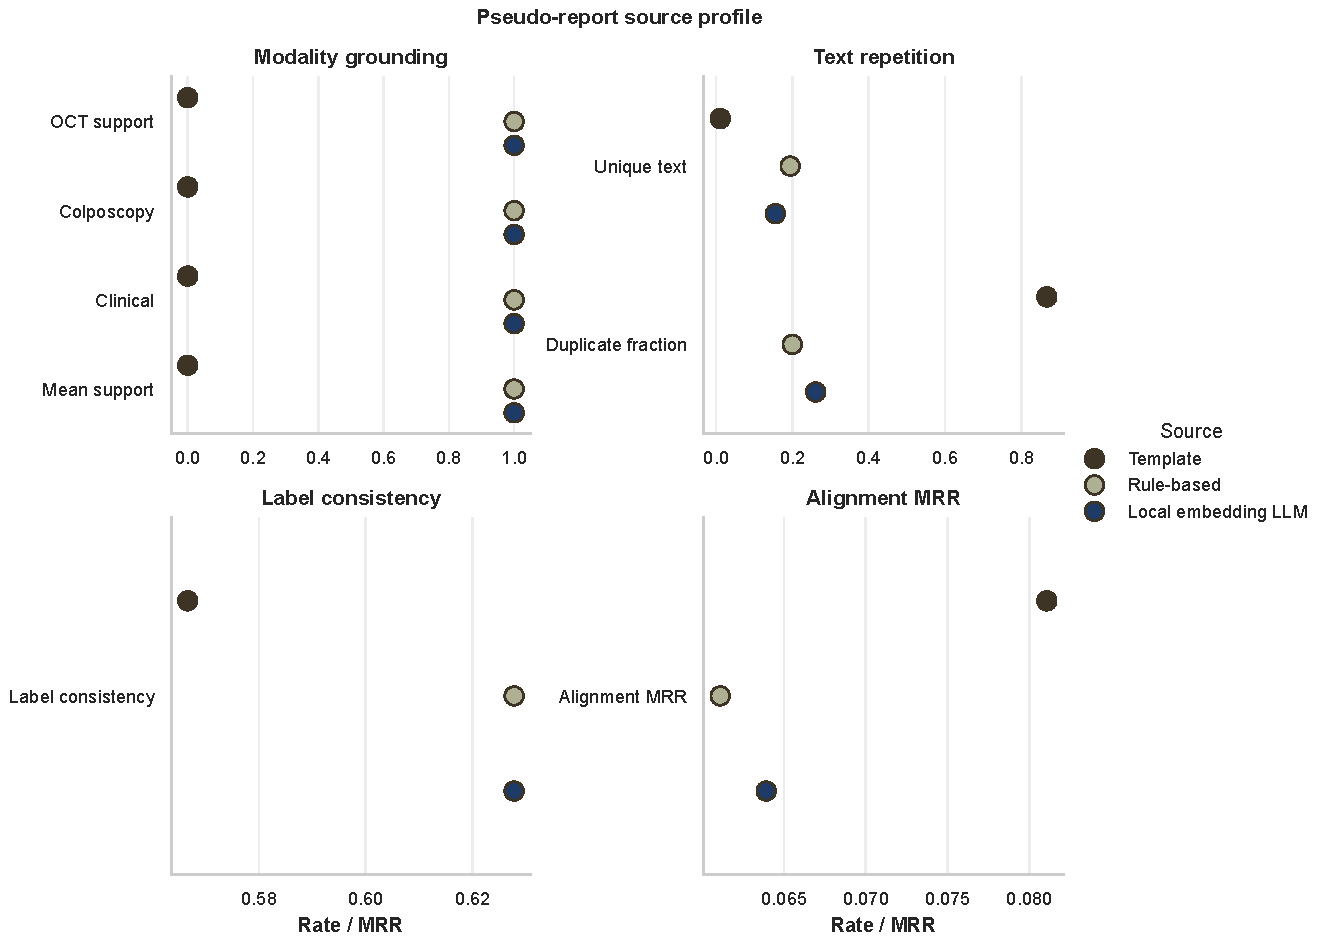
\includegraphics[width=\linewidth]{final_Fig/Figure_theme1_pseudo_report_source_comparison.pdf}
  \caption{Comparison of structured pseudo-report sources. The analysis contrasts label-template, rule-based, and local embedding-assisted structured reports in terms of section completeness, modality support, label consistency, and textual diversity.}
  \label{fig:pseudo_source_comparison}
\end{figure}

The rule-based and local embedding-assisted generators both preserved OCT, colposcopy, and clinical section support, with mean modality support of 1.000. They also reached the same mean label-consistency value of 0.628. The difference from the label-template control was not only quantitative. The generated sections remained tied to modality evidence and did not collapse into repeated label descriptions. These results support pseudo reports as weak semantic anchors for representation learning. They do not support using pseudo reports as replacements for clinician-authored documentation.

External provider experiments were retained as source-configurability audits. They assessed whether the structured completion layer could be implemented through alternative API-accessible language models under the same schema and privacy controls. All reported provider cohorts produced schema-valid structured outputs. The extended 100-case GPT-5.5 audit produced 100 valid reports, with section completeness 0.810, modality support 0.810, contradiction rate 0.050, and hallucination rate 0.000. Other providers were treated as pilot feasibility cohorts rather than head-to-head rankings. These results support source replaceability of the completion layer, not a claim that external API reports define the primary MOSAIC training source.

\subsubsection{Report-Supervision Scarcity}
\label{subsec:scarcity_results}

The second weak-oracle ablation reduced the amount of available real-report supervision. This experiment tests whether pseudo-report completion is most useful when report supervision is scarce. Table~\ref{tab:scarcity_curve} and Figure~\ref{fig:scarcity_curve} show a consistent pattern. At 10\% real-report availability, the LCAD-augmented surrogate achieved AUROC 0.808 and F1 0.500. The corresponding real-report-only surrogate achieved AUROC 0.630 and F1 0.316. At full real-report availability, the augmented surrogate also remained higher, with AUROC 0.838 and F1 0.542 compared with AUROC 0.799 and F1 0.471.

\begin{table*}[!htbp]
  \centering
  \caption{Report-supervision scarcity curve using a lightweight downstream surrogate.}
  \label{tab:scarcity_curve}
  \scriptsize
  \begin{threeparttable}
  \resizebox{\linewidth}{!}{%
  \begin{tabular}{llrrrrr}
    \toprule
    \textbf{Real-report fraction} & \textbf{Setup} & \textbf{Train (\(n\))} & \textbf{Real (\(n\))} & \textbf{Pseudo (\(n\))} & \textbf{AUROC} & \textbf{F1} \\
    \midrule
    \multirow{2}{*}{1.00} & LCAD-augmented surrogate  & 1,325 & 520 & 805 & \textbf{0.838} & \textbf{0.542} \\
                          & Real-report-only surrogate & 520   & 520 & 0   & 0.799 & 0.471 \\
    \addlinespace[2pt]
    \multirow{2}{*}{0.50} & LCAD-augmented surrogate  & 1,065 & 260 & 805 & \textbf{0.826} & \textbf{0.526} \\
                          & Real-report-only surrogate & 260   & 260 & 0   & 0.776 & 0.442 \\
    \addlinespace[2pt]
    \multirow{2}{*}{0.25} & LCAD-augmented surrogate  & 935   & 130 & 805 & \textbf{0.811} & \textbf{0.485} \\
                          & Real-report-only surrogate & 130   & 130 & 0   & 0.736 & 0.383 \\
    \addlinespace[2pt]
    \multirow{2}{*}{0.10} & LCAD-augmented surrogate  & 857   & 52  & 805 & \textbf{0.808} & \textbf{0.500} \\
                          & Real-report-only surrogate & 52    & 52  & 0   & 0.630 & 0.316 \\
    \bottomrule
  \end{tabular}%
  }
  \end{threeparttable}
\end{table*}

\begin{figure}[!htbp]
  \centering
  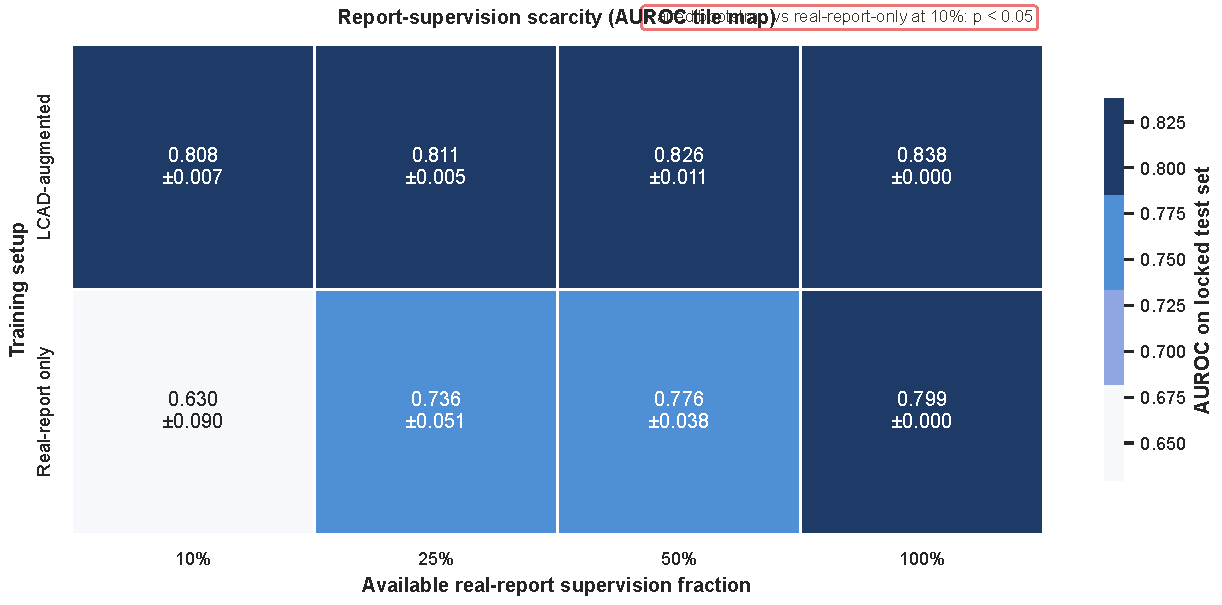
\includegraphics[width=\linewidth]{final_Fig/Figure_theme1_report_supervision_scarcity_curve.pdf}
  \caption{Effect of report-supervision scarcity on downstream surrogate performance. AUROC and F1 are compared between real-report-only learning and pseudo-report-augmented learning as the proportion of clinician-authored reports is reduced.}
  \label{fig:scarcity_curve}
\end{figure}

The scarcity curve matches the cohort-level bottleneck. Pseudo-report augmentation helped most when image and structured clinical data were available but report supervision was limited. The result supports LCAD as a mechanism for retaining report-missing cases in semantic learning. It does not imply that pseudo reports are equivalent to real reports.

\FloatBarrier

\subsection{Ablation and Sensitivity Analysis of Report-Section Alignment}
\label{subsec:alignment_results}

The next experiments evaluated whether report sections improved semantic organisation across modalities. OCT embeddings were matched to \texttt{oct\_findings}, colposcopy embeddings to \texttt{colposcopy\_findings}, clinical embeddings to \texttt{clinical\_context}, and fused representations to \texttt{impression}. Table~\ref{tab:theme1_alignment_ablation} reports retrieval metrics for the alignment ablation, and Figure~\ref{fig:alignment_retrieval_mrr} visualises the section-wise retrieval pattern.

\begin{table}[!htbp]
  \centering
  \caption{RASA alignment ablation using modality-section retrieval.}
  \label{tab:theme1_alignment_ablation}
  \small
  \begin{threeparttable}
  \begin{tabular}{lrrrr}
    \toprule
    \textbf{Model} & \textbf{Recall@1} & \textbf{Recall@5} & \textbf{Macro MRR} & \textbf{Positive cosine} \\
    \midrule
    Real-report only            & \textbf{0.0182} & \underline{0.0642} & \textbf{0.057} & \textbf{0.984} \\
    Pseudo-augmented LCAD       & 0.0139 & \textbf{0.0729} & \underline{0.055} & \textbf{0.984} \\
    MOSAIC-RASA backbone        & \underline{0.0148} & 0.0608 & 0.051 & \textbf{0.984} \\
    No section alignment        & 0.0052 & 0.0139 & 0.021 & 0.013 \\
    Simple concatenation fusion & 0.0035 & 0.0182 & 0.022 & 0.021 \\
    \bottomrule
  \end{tabular}
  \begin{tablenotes}[flushleft]
    \footnotesize
    \item Positive cosine is retained for completeness but is less discriminative than retrieval rank metrics in this audit.
  \end{tablenotes}
  \end{threeparttable}
\end{table}

\begin{figure}[!htbp]
  \centering
  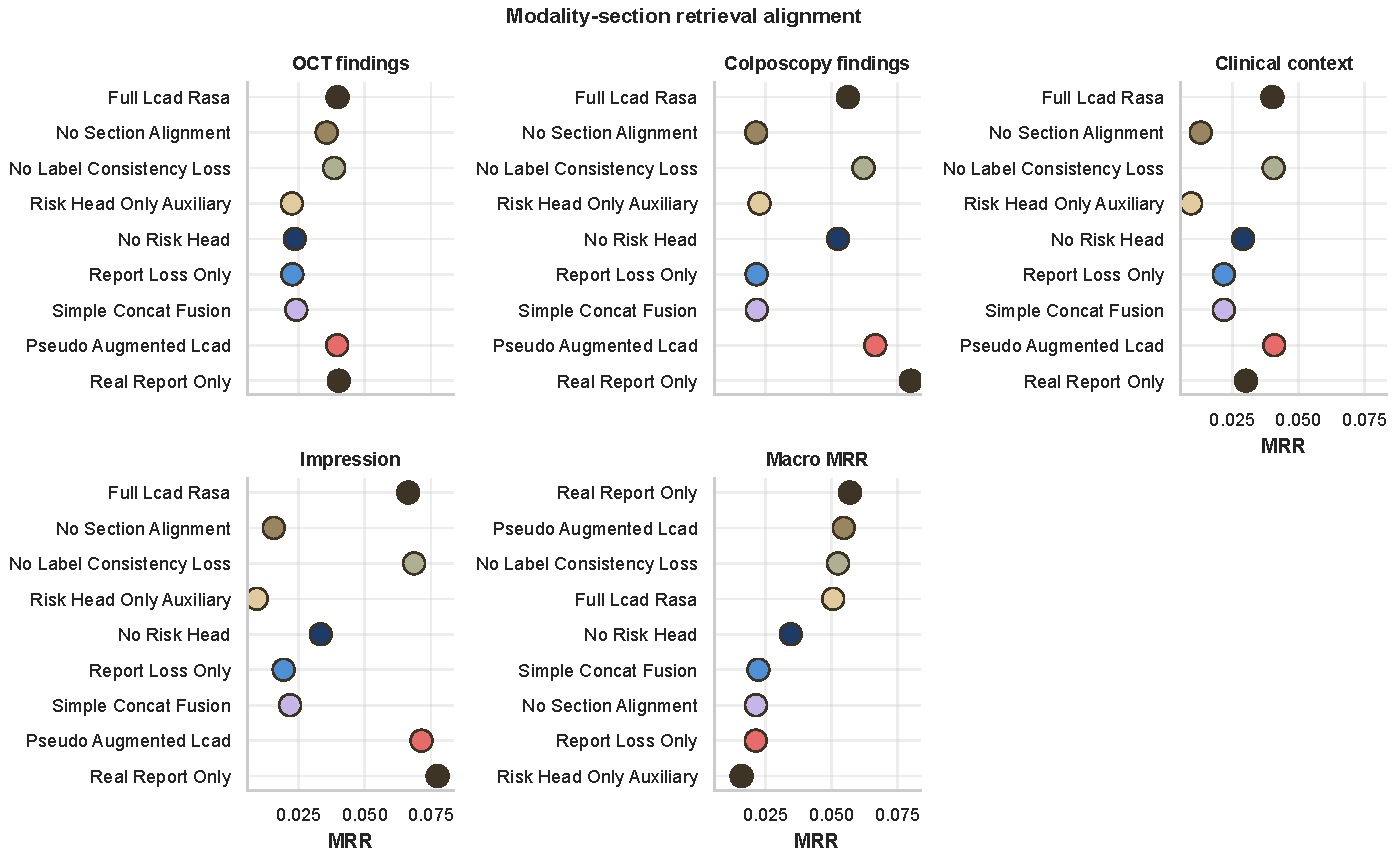
\includegraphics[width=\linewidth]{final_Fig/Figure_theme1_alignment_retrieval_mrr.pdf}
  \caption{Modality-section retrieval analysis for report-aware semantic alignment. Mean reciprocal rank quantifies whether modality-specific representations preferentially retrieve their corresponding report sections.}
  \label{fig:alignment_retrieval_mrr}
\end{figure}

The MOSAIC-RASA backbone achieved macro MRR 0.051 across the four report sections. Removing section alignment reduced macro MRR to 0.021, and simple concatenation remained low at 0.022. The real-report-only variant had the highest retrieval-only macro MRR of 0.057, which is expected because clinician-authored reports provide stronger semantic anchors when present.

The absolute retrieval scores remained low. The alignment result should therefore be interpreted as a relative semantic-organisation audit rather than evidence of high-fidelity retrieval. The value of MOSAIC is not that pseudo reports outperform real reports. Its value is that pseudo-report supervision extends report-guided alignment to cases for which multimodal evidence exists but archived reports are missing.

\subsubsection{Parameter Sensitivity and Component Ablations}
\label{subsec:parameter_component_results}

Computer-science evaluation also requires evidence about design sensitivity. Table~\ref{tab:extended_ablation_audit_summary} summarises the key mechanism checks. The alignment-weight sweep showed that \(\lambda_{\mathrm{align}}=0.20\) gave the best sweep AUROC of 0.776. The no-alignment setting reached 0.766, and the largest tested alignment weight reached 0.764. This pattern suggests that section alignment contributes a bounded optimisation signal. It does not act as a standalone semantic retrieval engine.

The modality ablations showed that different evidence streams were not interchangeable. Colposcopy plus clinical instruction reached AUROC 0.850. OCT alone reached AUROC 0.740, and clinical instruction alone reached AUROC 0.683. The component ablation also showed that the risk head was essential for prediction, while section alignment mainly affected semantic organisation and operating-point behaviour.

\begin{table*}[!htbp]
  \centering
  \caption{Condensed mechanism, parameter, and efficiency audits. These analyses support interpretation of the primary result but do not redefine the main MOSAIC model.}
  \label{tab:extended_ablation_audit_summary}
  \scriptsize
  \begin{threeparttable}
  \resizebox{\linewidth}{!}{%
  \begin{tabular}{p{3.4cm}p{5.6cm}p{7.0cm}}
    \toprule
    \textbf{Audit family} & \textbf{Key result} & \textbf{Interpretation} \\
    \midrule
    Provider-source feasibility & All evaluated provider cohorts produced schema-valid reports. In the 100-case GPT-5.5 audit, section completeness was 0.810, modality support was 0.810, contradiction rate was 0.050, and hallucination rate was 0.000. & Structured completion is source-configurable. External providers are feasibility audits, not the primary MOSAIC training source. \\
    Alignment-weight sensitivity & \(\lambda_{\mathrm{align}}=0.20\) gave the best sweep AUROC 0.776; no alignment reached 0.766; the largest alignment weight reached 0.764. & Section alignment adds a bounded optimisation signal and should not be interpreted as a standalone retrieval capability. \\
    Input-modality ablation & Colposcopy plus clinical instruction reached AUROC 0.850; OCT only reached 0.740; clinical instruction only reached 0.683. & Colposcopy carried strong signal, while OCT and clinical variables contributed complementary evidence. \\
    RASA component ablation & Variants without the risk head or using report loss only dropped to AUROC 0.750. Removing section alignment preserved AUROC in the legacy component table but reduced F1 and weakened retrieval alignment. & The risk head is necessary for discrimination; section alignment mainly supports semantic organisation and operating-point behaviour. \\
    Semantic-tag controls & MOSAIC-Tag reached AUROC 0.878. Random tag query fell to 0.853; train-label prior and random label-bank controls collapsed to the backbone at 0.856; same-centre-excluded retrieval weakened to 0.864. & The cleaned tag result is compatible with semantic retrieval, but it remains a secondary audit rather than a primary model. \\
    Pseudo-report QC controls & Downstream AUROC was unchanged across no-QC, QC-pass, QC-score, pseudo-confidence, and QC-confidence strategies. In the failure-enriched stress test, corrupted pseudo reports had pass rate 0.742 and severe-error flag rate 0.258. & QC is mainly a filtering and safety mechanism, not a downstream AUROC-improvement claim. \\
    Stability and masking validation & Multi-seed MOSAIC-RASA AUROC was 0.776 with SD 0.004. Modality-conditioned generation improved label consistency and ROUGE-L compared with label-only generation. & The pipeline was stable under repeated seeds, and report text remained more modality-responsive than label-only text. \\
    Scale and storage & The pipeline processed 1,897 cases, 137,591 image files, and 5,691 embedding files. Embedding storage was 47.349 MB, and publishable checkpoints were approximately 80 MB. & MOSAIC is tractable at the reported cohort scale and does not require storing large per-case retrieval artefacts at inference time. \\
    \bottomrule
  \end{tabular}%
  }
  \begin{tablenotes}[flushleft]
    \footnotesize
    \item Detailed provider routes, latency, cost estimates, file-level audits, and legacy protocol-harmonisation values are reported in the supplementary reproducibility material.
  \end{tablenotes}
  \end{threeparttable}
\end{table*}

\FloatBarrier

\subsection{Robustness, Leakage, and Failure-Mode Audits}
\label{subsec:robustness_stress_results}

The robustness experiments define where the current framework is informative and where its claims should stop. They test high-grade proxy behaviour, semantic-tag leakage controls, pseudo-report QC failure detection, perturbation response, and centre shift.

\subsubsection{CIN3+ Proxy Safety-Oriented Audit}
\label{subsec:cin3_proxy_safety_results}

We added a CIN3+ proxy audit because cervical-screening triage must consider high-grade disease safety. The proxy counted explicit CIN3/CIN 3, AIS, or carcinoma wording as CIN3+. Generic high-grade language alone was not counted. The endpoint is therefore a conservative pathology-text proxy and is used only as a retrospective safety-oriented audit.

Under the CIN2+ validation-F1 operating point, MOSAIC detected 17 of 20 proxy CIN3+ cases in the locked test set. Proxy CIN3+ sensitivity was 0.850, specificity was 0.903, NPV was 0.988, and there were three false negatives. At the validation-selected high-sensitivity operating point targeting proxy CIN3+ sensitivity \(\geq 0.95\), MOSAIC detected 19 of 20 proxy CIN3+ cases. This reduced false negatives to one but increased positive calls from 43 to 66 and lowered specificity to 0.825 (Table~\ref{tab:cin3_proxy_safety}).

\begin{table*}[!htbp]
  \centering
  \caption{CIN3+ proxy safety-oriented threshold audit on the locked test set.}
  \label{tab:cin3_proxy_safety}
  \scriptsize
  \begin{threeparttable}
  \resizebox{\linewidth}{!}{%
  \begin{tabular}{llrrrrrr}
    \toprule
    \textbf{Model} & \textbf{Operating point} & \textbf{AUROC} & \textbf{Sensitivity} & \textbf{Specificity} & \textbf{NPV} & \textbf{FN} & \textbf{Positive calls} \\
    \midrule
    MOSAIC & CIN2+ validation-F1 threshold & \textbf{0.954} & \textbf{0.850} & 0.903 & \textbf{0.988} & \textbf{3} & 43 \\
    MOSAIC & proxy CIN3+ high-sensitivity threshold & \textbf{0.954} & \textbf{0.950} & 0.825 & \textbf{0.995} & \textbf{1} & 66 \\
    MOSAIC-RASA backbone & CIN2+ validation-F1 threshold & 0.890 & 0.800 & 0.821 & 0.982 & 4 & 64 \\
    CLIP-style contrastive baseline & CIN2+ validation-F1 threshold & 0.937 & 0.700 & \textbf{0.937} & 0.977 & 6 & 31 \\
    Clinical-only HistGradientBoosting & CIN2+ validation-F1 threshold & 0.859 & 0.700 & 0.862 & 0.975 & 6 & 51 \\
    Clinical-only logistic regression & CIN2+ validation-F1 threshold & 0.869 & 0.650 & 0.851 & 0.970 & 7 & 53 \\
    \bottomrule
  \end{tabular}%
  }
  \begin{tablenotes}[flushleft]
    \footnotesize
    \item The locked test set contained 20 proxy CIN3+ cases under the conservative pathology-text rule. The high-sensitivity threshold was selected on the validation split for MOSAIC only. External baseline validation predictions were not available for this audit, so no test-tuned high-sensitivity threshold is reported for those rows.
  \end{tablenotes}
  \end{threeparttable}
\end{table*}

These results support retrospective risk stratification. They do not establish clinical triage safety. A prospectively locked and clinically curated CIN3+ endpoint is required before any prospective triage claim.

\subsubsection{Semantic-Tag and Leakage-Control Audits}
\label{subsec:llm_semantic_tag_results}

The semantic-tag audit tested whether explicit modality-specific tags could support the same train-only retrieval protocol without introducing leakage. A strict leakage screen was applied to \texttt{safe\_text}, tag text, normalised summary fields, tag columns, path-like strings, and identifier-like tokens. The initial uncleaned tag input was excluded because it contained target- or identifier-like metadata fields. After redaction and rule-tag regeneration, all 1,897 cases passed the leakage audit. Train, validation, and test splits had zero cases with forbidden target-derived terms, path-like tokens, or identifiers.

No LLM API key or local LLM endpoint was configured for semantic tagging in the execution environment. LLM-specific rows are therefore treated as unavailable. The deterministic rule-tag fallback is reported only as an implementation and leakage-control audit.

Rule-tag retrieval alone achieved AUROC 0.724, AUPRC 0.349, and F1 0.480. When fused with the RASA backbone, MOSAIC-Tag achieved AUROC 0.878, AUPRC 0.695, and F1 0.556. Its paired AUROC gain over MOSAIC-RASA was 0.023 (95\% CI 0.003--0.042; two-sided \(p=0.020\)). Random tag queries, train-label priors, and random label banks removed the gain. MOSAIC-Tag is therefore retained as a secondary audit of the semantic-prior mechanism. It does not replace the primary MOSAIC result.

\subsubsection{Quality-Control Stress Test}
\label{subsec:qc_stress_results}

The retrospective QC ablation did not materially change downstream AUROC. QC is therefore not interpreted as a discrimination-improving component. Its intended role is different: it should flag, down-weight, or reject unsafe pseudo-report supervision.

We tested this role through a failure-enriched stress audit. Existing pseudo reports were corrupted with label--impression contradictions, unsupported high-grade terminology, modality swaps, missing sections, modality hallucination, duplicated template text, inconsistent recommendations, and shuffled sections. The v2 audit added a deterministic modality--section consistency detector for OCT, colposcopy, and clinical sections. The corrupted pseudo reports had a pass rate of 0.742 and severe-error flag rate of 0.258, while clean pseudo reports had pass rate 1.000 and severe-error flag rate 0.000 (Table~\ref{tab:qc_failure_stress_test}). This supports QC as a filtering mechanism rather than an AUROC-improvement claim.

\begin{table}[!htbp]
  \centering
  \caption{Failure-enriched QC stress-test v2 audit.}
  \label{tab:qc_failure_stress_test}
  \small
  \begin{threeparttable}
  \begin{tabular}{p{5.0cm}rp{5.2cm}}
    \toprule
    \textbf{Stress-test metric} & \textbf{Value} & \textbf{Interpretation} \\
    \midrule
    Clean pseudo-report QC pass rate & 1.000 & clean baseline retained \\
    Corrupted pseudo-report QC pass rate & 0.742 & corrupted variants partly rejected or down-weighted \\
    Mean QC score, clean vs corrupted & 1.000 vs 0.855 & corrupted reports down-weighted \\
    Severe-error flag rate, clean vs corrupted & 0.000 vs 0.258 & severe failures enriched among corrupted reports \\
    Contradiction detection rate & 1.000 & expected contradiction flags detected \\
    Hallucination detection rate & 0.999 & unsupported terminology or missing-modality evidence detected \\
    Missing-section detection rate & 1.000 & empty required sections detected \\
    Modality-swap detection rate & 1.000 & modality--section consistency detector captured OCT--colposcopy swaps and shuffled sections \\
    Duplicate-template detection rate & 1.000 & repeated template text detected \\
    \bottomrule
  \end{tabular}
  \begin{tablenotes}[flushleft]
    \footnotesize
    \item The stress test used all 1,153 pseudo-report candidates and the v2 QC function. No retraining under corrupted reports was performed, and no LLM verifier comparison is claimed.
  \end{tablenotes}
  \end{threeparttable}
\end{table}

\FloatBarrier

\subsection{Perturbation Sensitivity and Modality Dependence}
\label{subsec:perturbation_results}

Perturbation analysis tested whether generated report sections responded to their expected evidence streams. Removing or shuffling a modality produced the largest degradation in the corresponding section. Masking OCT produced a 0.743 drop in the OCT findings section. Masking colposcopy produced a 1.000 drop in the colposcopy findings section. Masking clinical instruction produced a 0.833 drop in the clinical-context section (Table~\ref{tab:perturbation_matrix}).

\begin{table*}[!htbp]
  \centering
  \caption{Perturbation sensitivity matrix. Drops are relative to normal decoding.}
  \label{tab:perturbation_matrix}
  \scriptsize
  \begin{threeparttable}
  \resizebox{\linewidth}{!}{%
  \begin{tabular}{lrrrrr}
    \toprule
    \textbf{Condition} & \textbf{OCT drop} & \textbf{Colposcopy drop} & \textbf{Clinical drop} & \textbf{Report drop} & \textbf{\(|\Delta\mathrm{risk}|\)} \\
    \midrule
    Mask OCT             & 0.743 & 0.000 & 0.000 & 0.211 & 0.053 \\
    Shuffle OCT          & 0.839 & 0.000 & 0.000 & 0.196 & 0.020 \\
    Mask Colposcopy      & 0.000 & \textbf{1.000} & 0.000 & 0.177 & 0.148 \\
    Shuffle Colposcopy   & 0.000 & 0.999 & 0.000 & 0.131 & 0.008 \\
    Mask Instruction     & 0.000 & 0.000 & 0.833 & 0.179 & 0.027 \\
    Shuffle Instruction  & 0.000 & 0.000 & 0.917 & 0.141 & 0.000 \\
    Mask Visual          & 0.743 & \textbf{1.000} & 0.000 & \underline{0.320} & \underline{0.313} \\
    Label-only inference & 0.743 & \textbf{1.000} & 0.833 & \textbf{0.466} & \textbf{0.371} \\
    \bottomrule
  \end{tabular}%
  }
  \begin{tablenotes}[flushleft]
    \footnotesize
    \item Specificity hit was 1.000 for every perturbation condition and was removed as a non-informative duplicate column.
  \end{tablenotes}
  \end{threeparttable}
\end{table*}

\begin{figure}[!htbp]
  \centering
  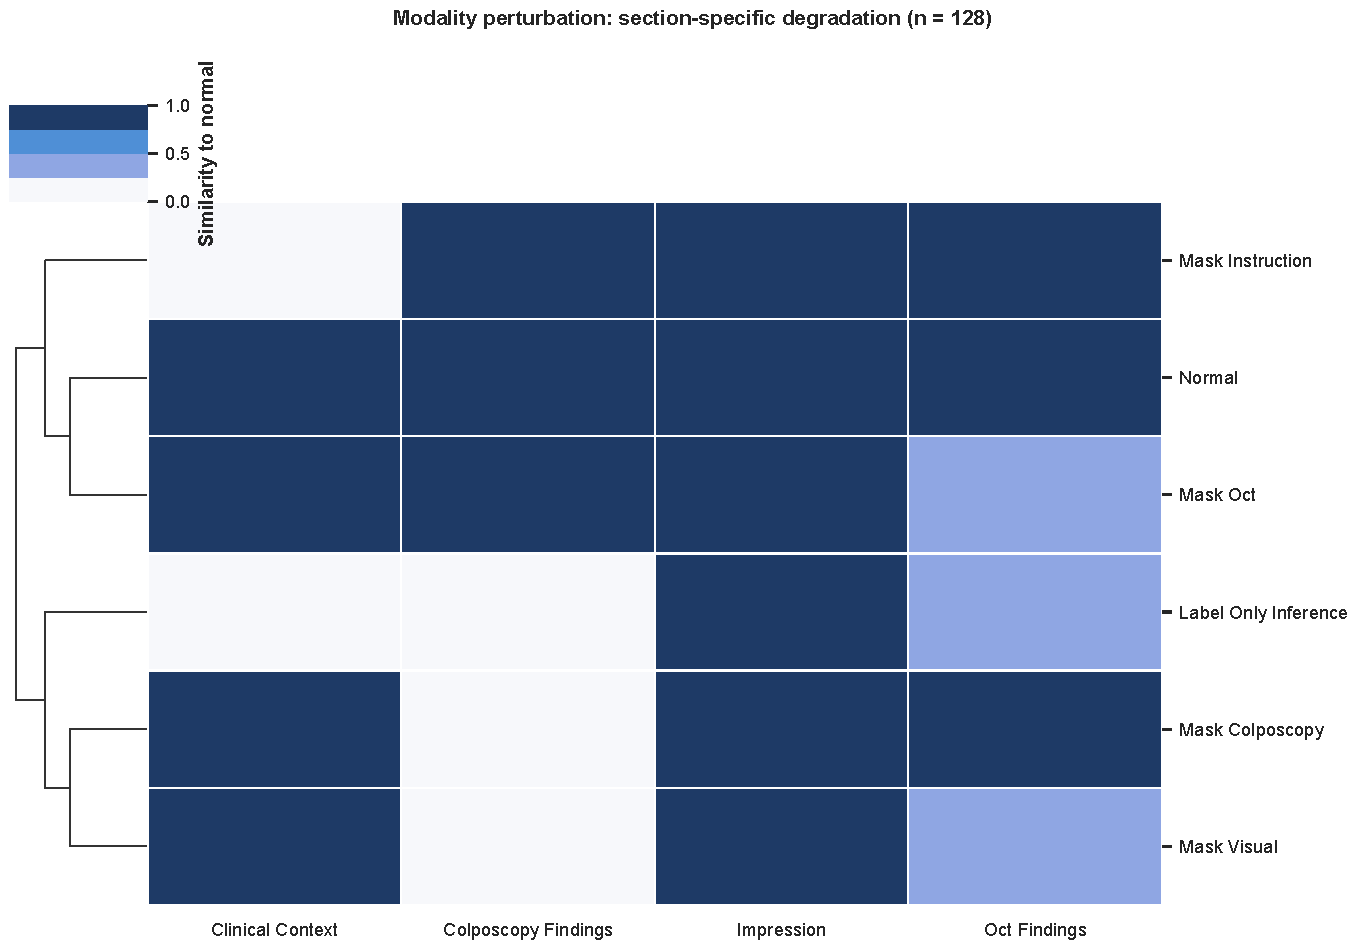
\includegraphics[width=\linewidth]{final_Fig/Figure3_modality_perturbation_heatmap.pdf}
  \caption{Report-section sensitivity under modality perturbations. The matrix summarises how masking or shuffling OCT, colposcopy, or clinical evidence changes similarity in the corresponding generated report sections.}
  \label{fig:perturbation_heatmap}
\end{figure}

\begin{figure}[!htbp]
  \centering
  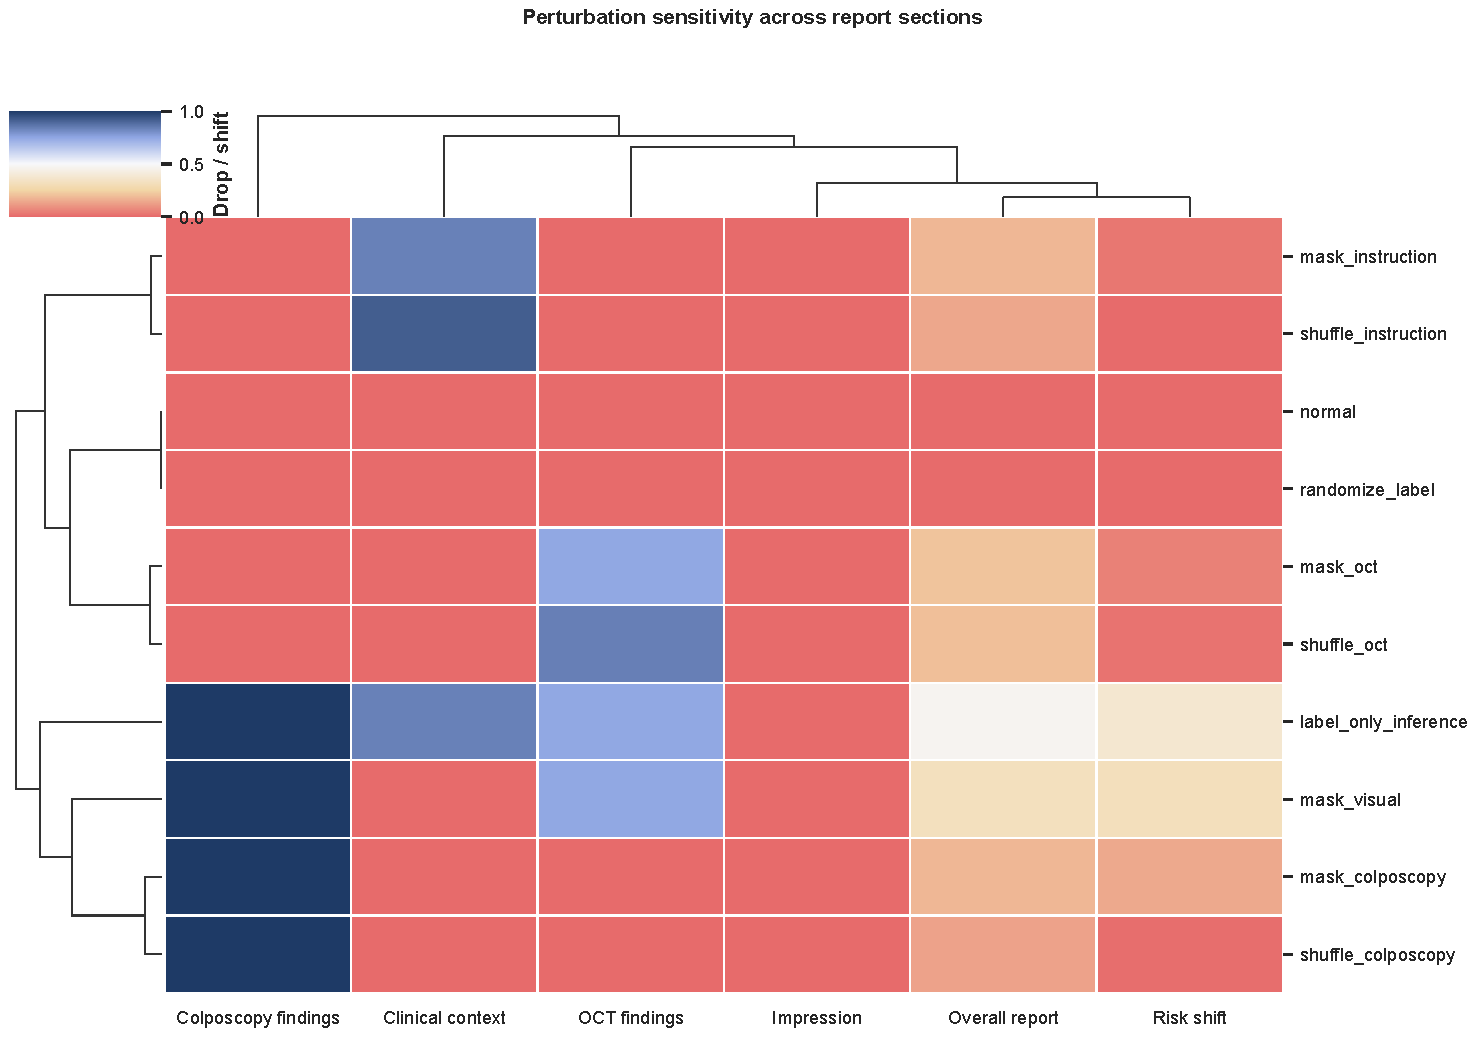
\includegraphics[width=\linewidth]{final_Fig/Figure_theme1_perturbation_sensitivity_matrix.pdf}
  \caption{Expanded perturbation sensitivity profiles. The matrix consolidates section-level degradation, report-level degradation, risk shift, and specificity of the expected modality-section response.}
  \label{fig:theme1_perturbation}
\end{figure}

Label-only inference produced the largest overall report drop (0.466) and the largest absolute risk shift (0.371). This helps separate modality-grounded report decoding from fixed-template schema filling. The analysis remains perturbational. It should not be interpreted as causal clinical explanation.

\FloatBarrier

\subsection{Centre Shift, Scalability, and Efficiency}
\label{subsec:loco_results}

Reference-stratified testing assessed whether held-out behaviour was confined to cases with archived reports. The MOSAIC-RASA backbone achieved AUROC 0.824 among cases with reference reports (\(n=108\)) and AUROC 0.850 among cases without reference reports (\(n=180\)). This suggests that the model was not restricted to the real-report subset. The analysis remains retrospective and conditioned on the available cohort composition.

Strict leave-one-centre-out evaluation was used as a centre-shift stress test. It was not used as an external-validation success criterion. Figure~\ref{fig:loco_heatmap} shows substantial centre-level heterogeneity. Under fixed quick-budget retraining, held-out AUROC was 0.702 for Enshi, 0.648 for Jingzhou, 0.500 for Shiyan, 1.000 for Wuhan Renmin, and 0.382 for Xiangyang. The Wuhan fold was small (\(n=13\)), so the apparent perfect AUROC is not interpreted as centre-invariant generalisation. Eval-only LOCO using a global checkpoint was analysed separately and was not pooled with strict LOCO retraining.

\begin{figure}[!htbp]
  \centering
  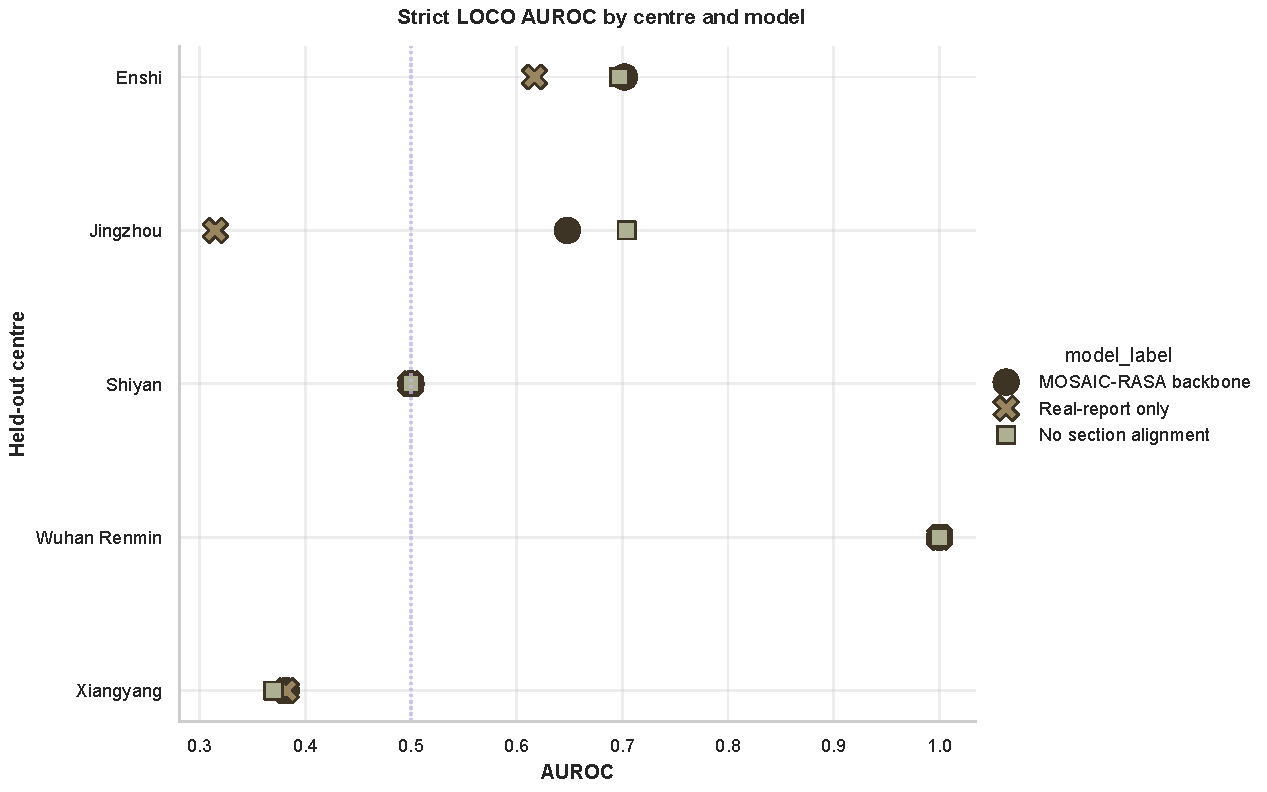
\includegraphics[width=1\linewidth]{final_Fig/fig_loco_heatmap.pdf}
  \caption{Leave-one-centre-out centre-shift stress-test evaluation across participating centres. The panels summarise centre-wise AUROC patterns and strict LOCO performance, illustrating the extent of distribution shift under centre-held-out evaluation.}
  \label{fig:loco_heatmap}
\end{figure}

The scale audit supports tractability at the reported cohort size. MOSAIC processed 137,591 image files and 5,691 embedding files. The embedding storage footprint was 47.349 MB, and publishable checkpoints were approximately 80 MB. A case-level embedding audit found no cross-split case, hashed-patient, or embedding-path leakage. Repeated raw colposcopy paths appeared only within the same split and were retained as a data-provenance caveat. These findings support MOSAIC as a reproducible retrospective analytics workflow. They also identify domain shift as a main limitation.

\FloatBarrier

\subsection{Summary of Evidence}
\label{subsec:results_summary_evidence}

The experiments support three bounded claims. First, QC-gated weak-oracle completion can retain report-missing cases for semantic learning when generated reports remain schema-constrained, modality-grounded, and separated from clinician-authored reports. Second, section-aware RASA provides a measurable alignment signal by linking modality-specific representations to corresponding report sections, although the low absolute retrieval scores limit the claim to relative semantic organisation. Third, train-only retrieval with validation-calibrated fusion improves the MOSAIC-RASA backbone on the locked held-out test set and remains competitive with the strongest same-split contrastive baseline.

The robustness audits define the limits of these claims. The framework is sensitive to report scarcity, semantic-tag leakage, pseudo-report corruption, modality perturbation, and centre shift. The current evidence supports MOSAIC as a retrospective, leakage-controlled analytics framework for report-imbalanced multimodal cervical screening data. It does not establish prospective clinical use, autonomous LLM decision-making, centre-invariant generalisation, causal reasoning, or conclusive superiority over all strong foundation-model baselines.









\section{Discussion}
\label{sec:discussion}

This study addresses a supervision bottleneck that is increasingly common in clinical big-data analytics. The five-centre cohort contained 1,897 multimodal cases and 137,591 evaluable image files, yet clinician-authored report supervision was sparse and strongly centre-dependent. The central problem was therefore not the absence of imaging evidence, but the uneven availability of semantic annotations that explain how multimodal findings are organised and interpreted. MOSAIC was designed for this setting: it converts incomplete report supervision into quality-controlled weak semantic priors, while keeping generated text separate from clinician-authored reports and pathology-derived endpoints.

A distinctive aspect of this work is the data setting itself. The privately curated cohort jointly contains OCT images, colposcopy images, structured HPV, TCT, and age variables, histopathology-derived endpoints, and incomplete report-level supervision across five centres. This provides a rare report-aware setting for cervical OCT analytics, where visual, structured, pathological, and textual evidence are linked at the case level but documented with unequal completeness across institutions. The resulting supervision imbalance is not a nuisance variable alone; it is the methodological problem that MOSAIC is built to address.

The weak-oracle formulation offers a controlled way to use this imperfect semantic evidence. LCAD retained report-missing cases by producing schema-constrained and modality-grounded pseudo reports with QC weighting, rather than excluding them from semantic learning. The label-template control showed that structural completeness alone was insufficient, since complete but repetitive text without modality support did not provide meaningful supervision. Rule-based and local embedding-assisted pseudo reports preserved modality-grounded sections and were most useful when real reports were scarce. These findings support pseudo reports as bounded weak semantic anchors, not as replacements for clinical documentation.

RASA further showed that report sections can provide an auditable organisation signal for cross-modal representation learning. The improvement in modality-section retrieval over no-section and simple-concatenation ablations indicates that OCT, colposcopy, clinical variables, and fused representations were better aligned with their corresponding report sections. The absolute retrieval scores remained low, however, and should not be interpreted as high-fidelity semantic retrieval or causal explanation. The appropriate interpretation is narrower: section-aware report structure provides a measurable and inspectable alignment signal under a stringent audit.

The strongest predictive evidence came from train-only retrieval-calibrated fusion. MOSAIC improved held-out AUROC from 0.856 for the MOSAIC-RASA backbone to 0.908 after validation-calibrated fusion, with a paired bootstrap AUROC gain of 0.053. This supports the value of retrieved report-derived priors when the semantic bank is restricted to training cases and the fusion parameters are selected on validation data only. The same-split baseline comparison also defines an important boundary. MOSAIC exceeded the CLIP-style contrastive baseline in point estimate, but the paired AUROC interval crossed zero. The result should therefore be read as evidence for a competitive and auditable semantic-prior framework, rather than as conclusive superiority over all strong multimodal baselines.

The role of LLMs in MOSAIC is deliberately bounded. LLM-assisted structuring is used to support offline weak semantic supervision and provider-feasibility auditing, not to produce autonomous diagnostic decisions. Real reports are preserved when available, pseudo reports are QC-weighted, and generated text is never used as pathology ground truth. The semantic-tag audit follows the same principle: because no LLM tag endpoint was configured in the current execution environment, deterministic rule tags were reported only as a separate leakage-control and mechanism audit. This distinction is important for interpreting MOSAIC as an LLM-assisted semantic-prior learning framework, rather than as an LLM diagnostic system.

Several limitations remain. The study is retrospective, and the locked held-out test set was drawn from the available five-centre cohort rather than from a prospectively collected external cohort. Expert physician scoring of generated report sections was not available, so report quality was evaluated through structural, QC, proxy, and perturbation audits. The CIN3+ analysis used a conservative pathology-text proxy and should not be treated as a prospectively curated safety endpoint. Strict leave-one-centre-out evaluation revealed substantial centre dependence, particularly in the Xiangyang fold, indicating that centre shift remains unresolved. In addition, provider prompts and run settings were recoverable from retained artefacts, but per-request API timestamps were not preserved in the exported provider tables. A generic retrieval-fusion control for non-MOSAIC baselines was also not executed because validation predictions for those baselines were unavailable under the locked protocol. These limitations motivate prospective validation, stronger centre-shift mitigation, physician-rated report-quality assessment, and integration with stronger contrastive pretraining.

Overall, MOSAIC contributes a leakage-controlled workflow for organising fragmented multimodal and textual evidence into auditable semantic priors. Its primary contribution is not autonomous report generation or clinical deployment, but a reproducible analytics framework for learning from incomplete, centre-dependent report supervision at scale. This framing is aligned with large-scale multimodal big-data analytics: the method studies how heterogeneous clinical evidence can be structured, audited, and used for retrospective risk stratification while keeping generated language within explicit methodological boundaries.

\section{Conclusion}
\label{sec:con}

Incomplete and unevenly distributed clinical reports are a practical obstacle for large-scale multimodal cervical screening analytics. They contain valuable semantic information about how imaging findings, structured clinical variables, and diagnostic impressions are connected, yet their sparse and centre-dependent availability makes them difficult to use as conventional supervision. MOSAIC addresses this problem by reframing incomplete report supervision as weak-oracle semantic prior learning. In a five-centre retrospective cohort of 1,897 cases with 137,591 evaluable image files, the framework retained report-missing cases through QC-gated pseudo-report completion, organised multimodal representations with report-section anchors, and converted train-only semantic retrieval into validation-calibrated risk fusion.

This design shifts the role of generated report text from replacement documentation to bounded semantic supervision. The primary held-out evaluation showed that MOSAIC achieved AUROC 0.908, AUPRC 0.741, and F1 0.736, with a paired AUROC gain of 0.053 over the MOSAIC-RASA backbone. More importantly, the improvement was obtained under explicit leakage control: real reports were not overwritten, pseudo reports were not treated as ground truth, the semantic bank was restricted to training cases, and fusion parameters were selected on validation data only. These results suggest that incomplete clinical-report evidence can be made useful for retrospective multimodal learning when it is structured, quality-gated, and audited rather than used as an unqualified textual label.

MOSAIC therefore contributes a controlled analytics framework for report-imbalanced multimodal cervical screening data, rather than an autonomous diagnostic system. The current evidence supports weak semantic supervision, section-aware alignment, and retrieval-calibrated fusion as reproducible mechanisms for retrospective risk modelling. It does not establish prospective clinical deployment, centre-invariant generalisation, autonomous LLM decision-making, or conclusive superiority over all strong contrastive baselines. Future work should validate the framework in prospectively collected cohorts, strengthen centre-shift robustness, incorporate physician-rated report-quality assessment, and evaluate non-report retrieval controls to further separate semantic-prior effects from generic neighbour-label memory.



% % BEGIN INTEGRATED_SUPPLEMENTARY_APPENDIX
% \clearpage
% \appendix
% \section{Supplementary Results and Audit Appendix}
% \label{app:integrated_supplementary_results}

% This appendix integrates the supplementary result package into the main manuscript so that the submission source remains self-contained. The standalone supplementary source was originally prepared as a separate LaTeX article beginning with the class declaration \verb|\documentclass[11pt,a4paper]{article}|. In the integrated manuscript, that declaration is reported here as source provenance rather than executed as a second document-class command, because the main manuscript already defines its document class in the preamble.

% The appendix is organised as a manuscript evidence chain rather than as a numbered experiment log. It first documents structured pseudo-report generation and provider feasibility, then gives protocol-harmonisation context for historical backbone results, semantic-tag leakage-control audits, RASA and modality ablations, extended baseline diagnostics, perturbation behaviour, centre-shift stress tests, multi-seed stability, report-safety summaries, masking validation, runtime measurements, and robustness visualisations. These materials support and qualify the main results in Section~\ref{sec:experiments_results}; they do not redefine the primary MOSAIC training source or introduce independent deployment claims.

% All appendix results follow the same retrospective, leakage-controlled boundary as the main text. They should be read as supporting audits for the primary conclusion that incomplete report supervision can be converted into auditable weak semantic priors under train-only retrieval and validation-locked fusion. They do not establish prospective clinical utility, autonomous LLM decision-making, unrestricted external generalisation, or direct superiority of LLM semantic tags.

% \subsection{Provider comparison for structured pseudo-report generation}
% \label{app:subsec:provider_comparison}
% \begin{table*}[!htbp]
%   \centering
%   \caption{Supplementary LLM provider comparison for structured pseudo-report generation.}
%   \label{app:tab:llm_provider_comparison}
%   \scriptsize
%   \begin{threeparttable}
%   \resizebox{\linewidth}{!}{%
%   \begin{tabular}{lrrrrrrr}
%     \toprule
%     \textbf{Source} & \textbf{Valid/req.} & \textbf{Section comp.} & \textbf{Modality supp.} & \textbf{Contradiction rate} & \textbf{Duplicate frac.} & \textbf{Alignment MRR} & \textbf{Latency (s)} \\
%     \midrule
%     Template              & 100/100 & 1.000 & 0.000 & \textbf{0.000} & 0.860 & 0.110 & \NA \\
%     Rule-based            & 100/100 & 1.000 & 1.000 & \underline{0.040} & \textbf{0.010} & 0.102 & \NA \\
%     Local embedding LLM   & 100/100 & 1.000 & 1.000 & \underline{0.040} & \textbf{0.010} & 0.098 & \NA \\
%     Qwen-Plus             & 10/10   & 1.000 & 1.000 & 0.600 & 0.100 & \underline{0.318} & 13.68 \\
%     GLM-4.7-Flash         & 10/10   & 1.000 & 0.933 & 0.300 & 0.100 & 0.295 & 25.06 \\
%     Gemini-3.1-Pro        & 9/9     & 1.000 & 1.000 & 0.444 & 0.111 & \textbf{0.366} & 25.70 \\
%     GPT-5.5               & 100/100 & 0.810 & 0.810 & 0.050 & 0.190 & 0.063 & \textbf{11.39} \\
%     \bottomrule
%   \end{tabular}%
%   }
%   \begin{tablenotes}[flushleft]
%     \footnotesize
%     \item Schema-valid rate was 1.000 and hallucination rate was 0.000 for all evaluated sources; these non-informative duplicate rows were omitted from the body of the table. Latency was measured only for API providers. GPT-5.5 had an estimated cost of US\$27.73 per 1,000 cases. Qwen-Plus, GLM-4.7-Flash, and Gemini-3.1-Pro were pilot cohorts; GPT-5.5 was the extended 100-case API cohort.
%   \end{tablenotes}
%   \end{threeparttable}
% \end{table*}

% \subsection{Quality-control summary for pseudo-report candidates}
% \label{app:subsec:pseudo_report_qc_summary}
% \begin{table}[!htbp]
%   \centering
%   \caption{Supplementary Table S8. LLM pseudo-report quality-control summary.}
%   \label{app:tab:s8_llm_pseudo_report_qc}
%   \small
%   \begin{threeparttable}
%   \begin{tabular}{lrr}
%     \toprule
%     \textbf{Source} & \textbf{$n$} & \textbf{Pass rate} \\
%     \midrule
%     Mock pseudo reports & 1,153 & 1.000 \\
%     LLM pseudo reports  & 1,153 & 1.000 \\
%     \bottomrule
%   \end{tabular}
%   \begin{tablenotes}[flushleft]
%     \footnotesize
%     \item Invalid placeholder entries and duplicated source-table metadata were removed. The quality-summary row also contained $n_{\mathrm{QC}}=1,153$ and pass rate = 1.000.
%   \end{tablenotes}
%   \end{threeparttable}
% \end{table}

% \subsection{Provider-level pseudo-report quality heatmap}
% \label{app:subsec:api_provider_summary}
% \begin{figure}[!htbp]
%   \centering
%   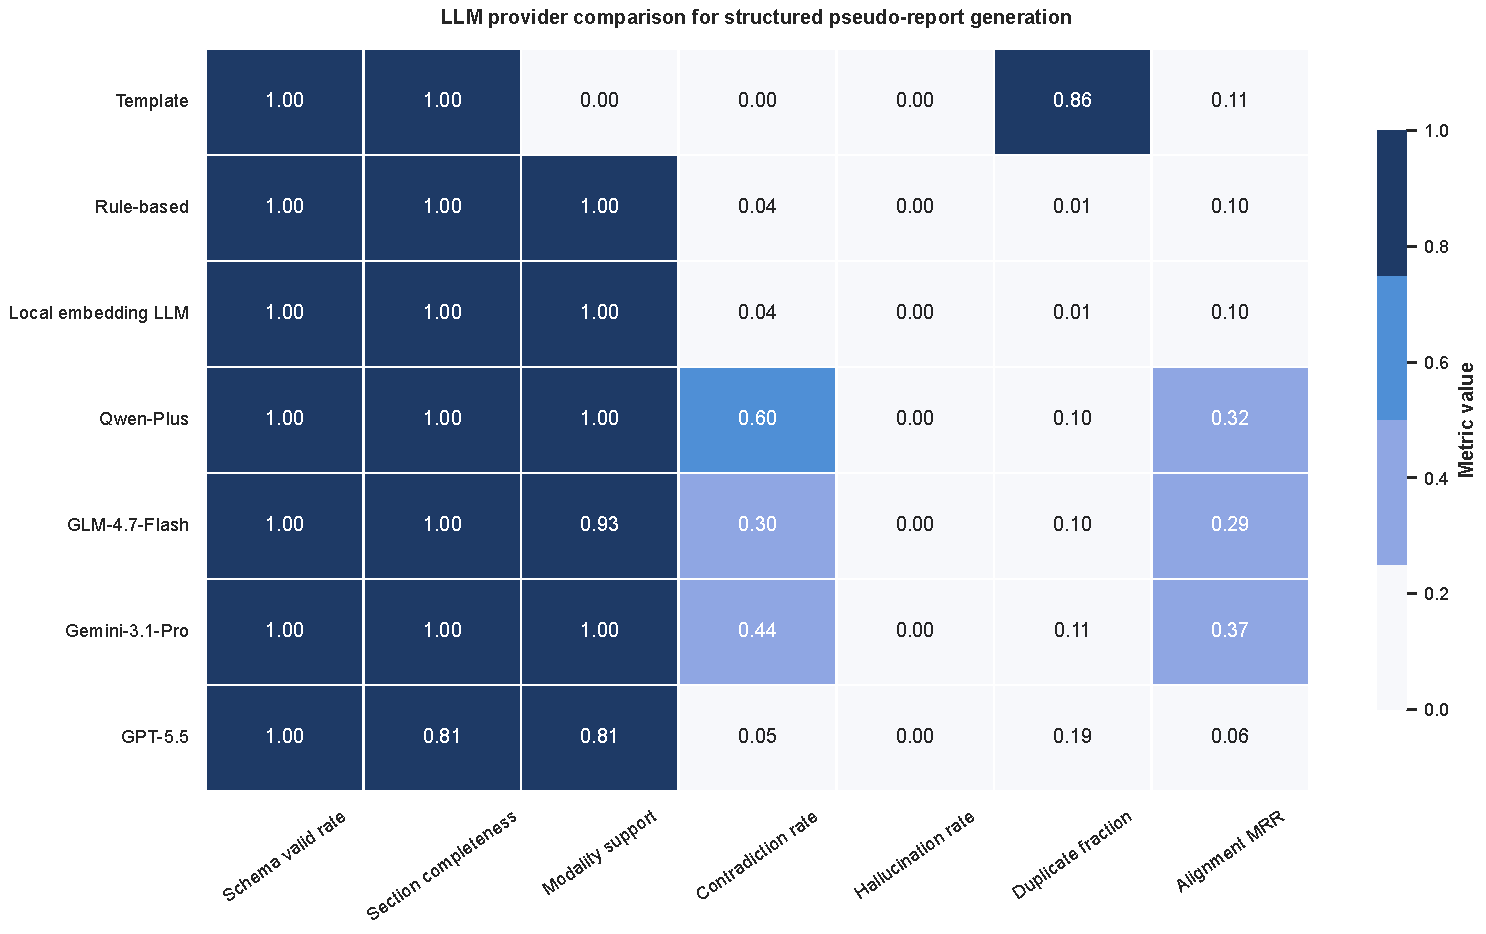
\includegraphics[width=\linewidth]{final_Fig/P8_llm_provider_comparison_heatmap.pdf}
%   \caption{Supplementary provider-level comparison for structured pseudo-report generation. The heatmap summarises schema adherence, section completeness, modality support, contradiction risk, duplication, alignment, latency, and cost across template, rule-based, local LLM, and external API-based sources.}
%   \label{app:fig:api_provider_summary_heatmap}
% \end{figure}

% \subsection{Stage 1 pseudo-report quality and risk diagnostics}
% \label{app:subsec:api_quality_diagnostics}
% \begin{figure}[!htbp]
%   \centering
%   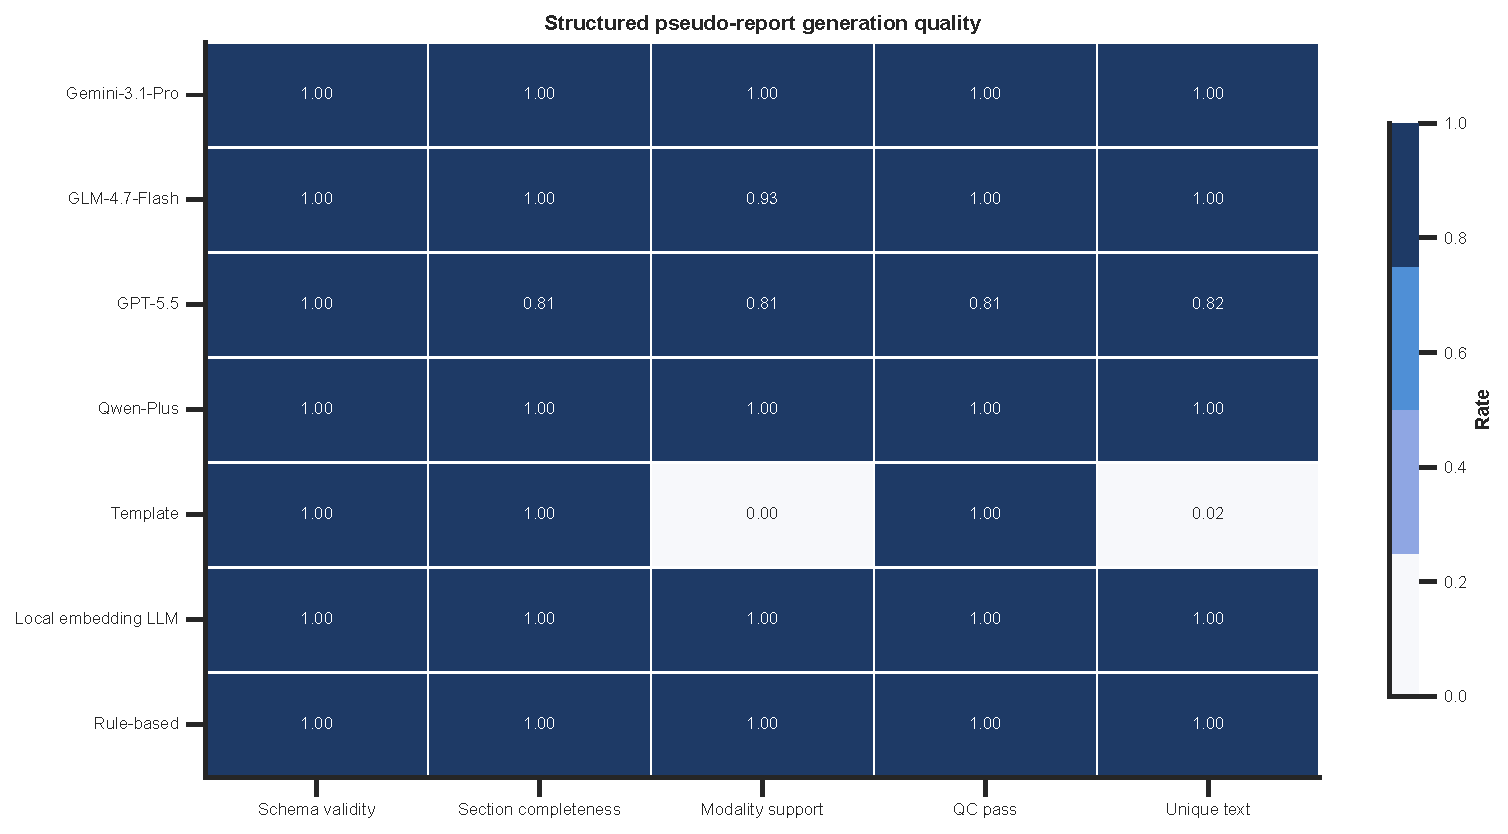
\includegraphics[width=\linewidth]{final_Fig/P1_stage1_quality_heatmap.pdf}
%   \hfill
%   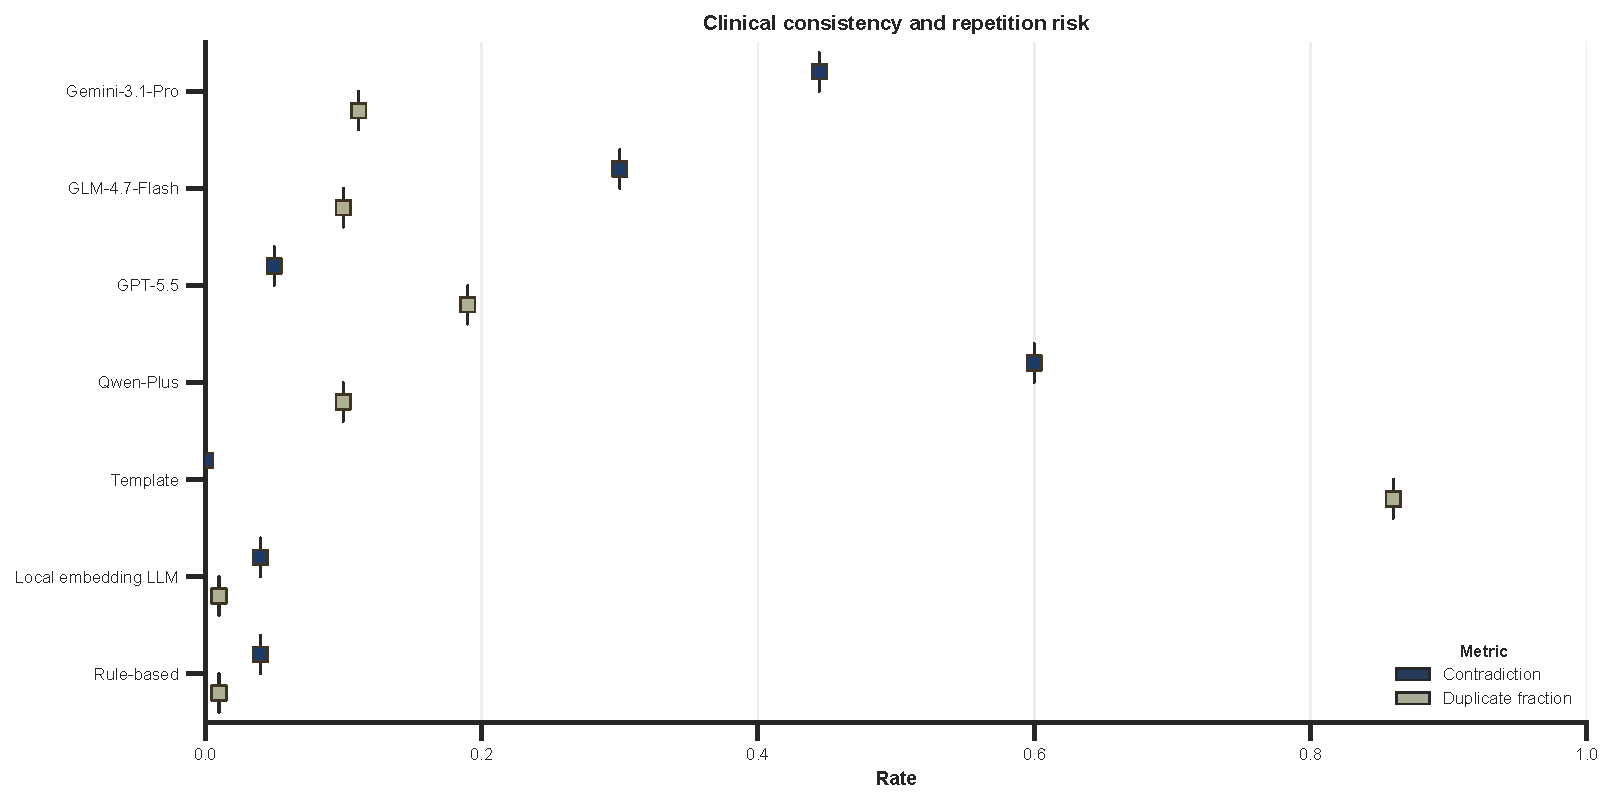
\includegraphics[width=\linewidth]{final_Fig/P2_stage1_quality_risk_bars.pdf}
%   \caption{Supplementary Stage 1 evaluation of pseudo-report generation quality across LLM providers. The panels summarise generation validity and completeness together with risk-oriented quality indicators, including modality support, contradiction rate, hallucination rate, and duplicate-text behaviour.}
%   \label{app:fig:api_quality_heatmap}
% \end{figure}

% \subsection{Operational reliability of external pseudo-report generation}
% \label{app:subsec:api_reliability}
% \begin{figure}[!htbp]
%   \centering
%   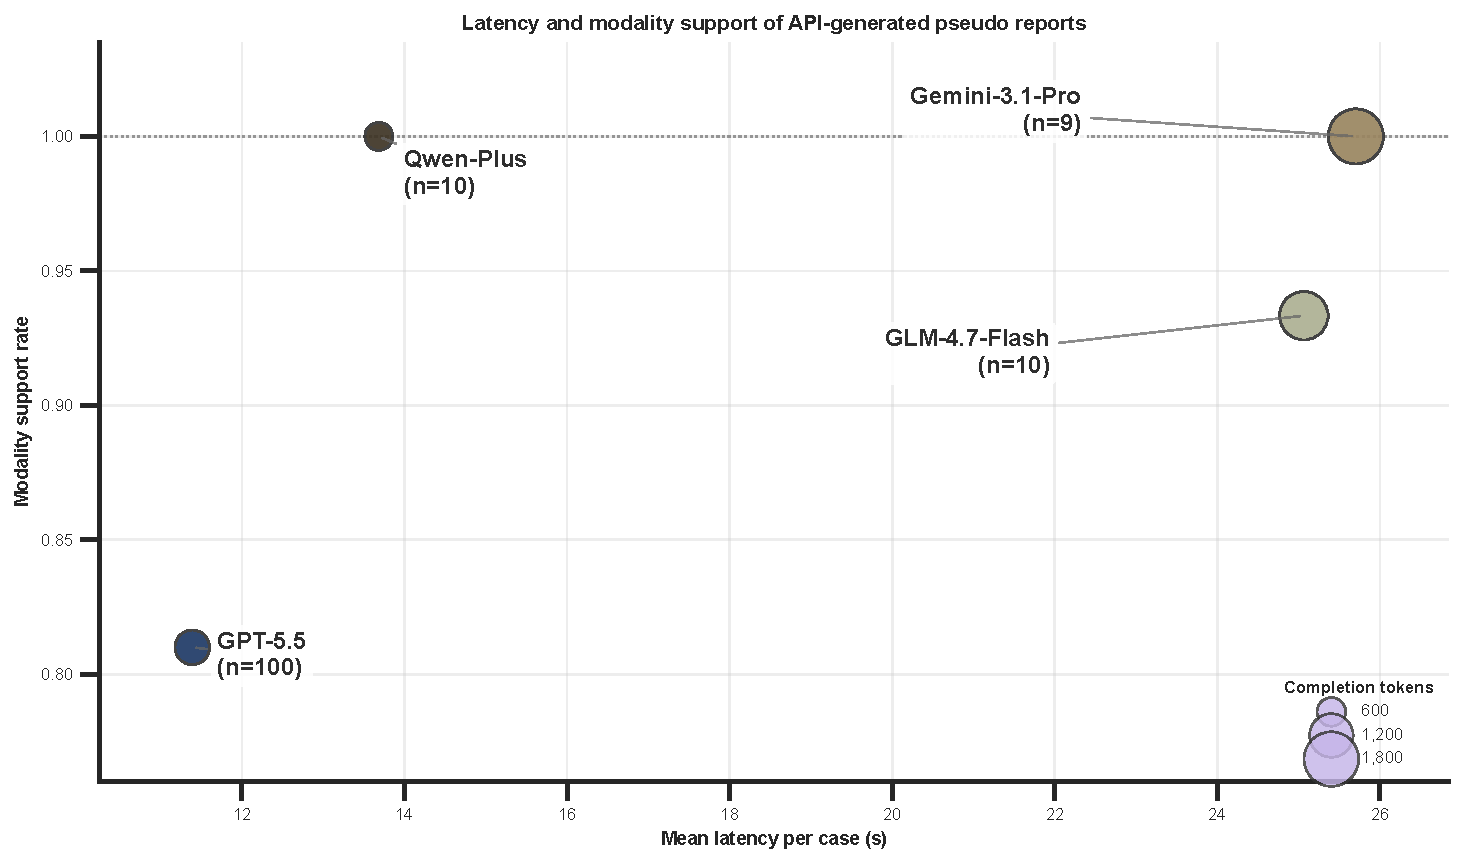
\includegraphics[width=\linewidth]{final_Fig/P3_stage1_latency_support_scatter.pdf}
%   \hfill
%   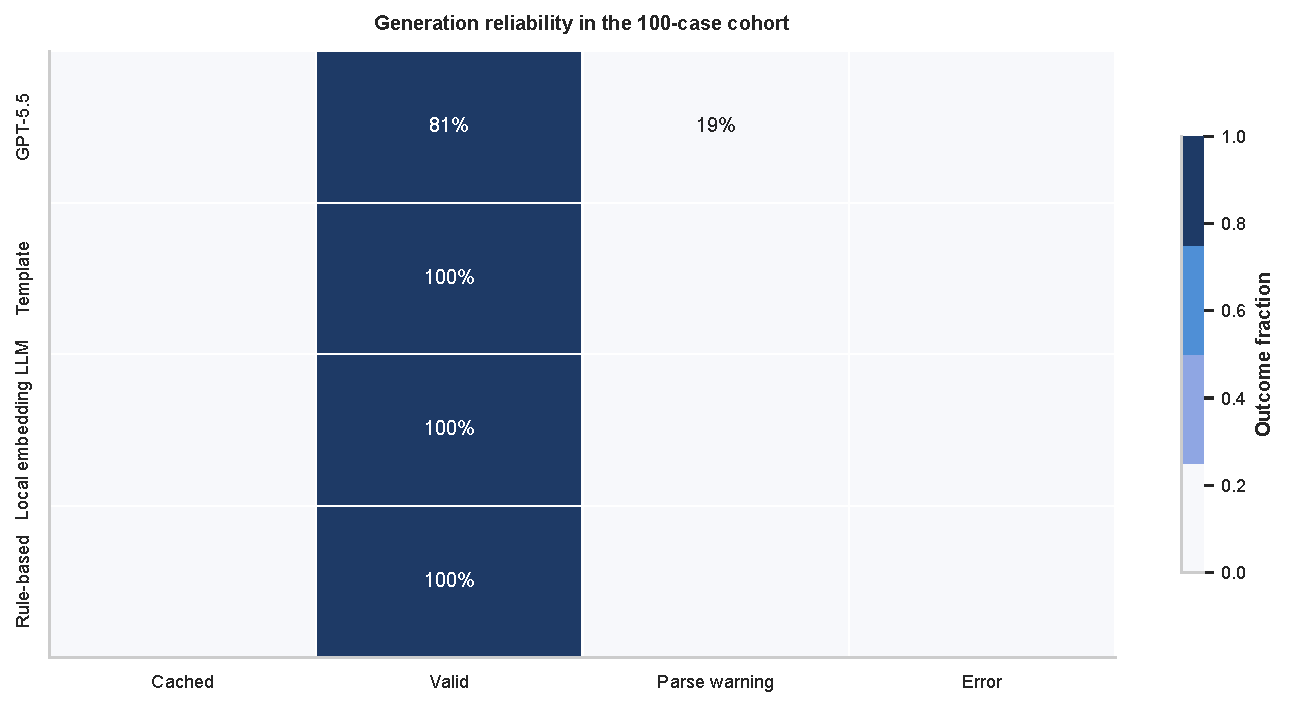
\includegraphics[width=\linewidth]{final_Fig/P4_stage1_generation_reliability.pdf}
%   \caption{Supplementary operational reliability of external pseudo-report generation. The panels relate generation latency to modality support and summarise request completion and schema-valid output rates across evaluated providers.}
%   \label{app:fig:api_reliability}
% \end{figure}

% \subsection{Provider-generated pseudo reports in modality-section retrieval}
% \label{app:subsec:api_alignment_summary}
% \begin{figure}[!htbp]
%   \centering
%   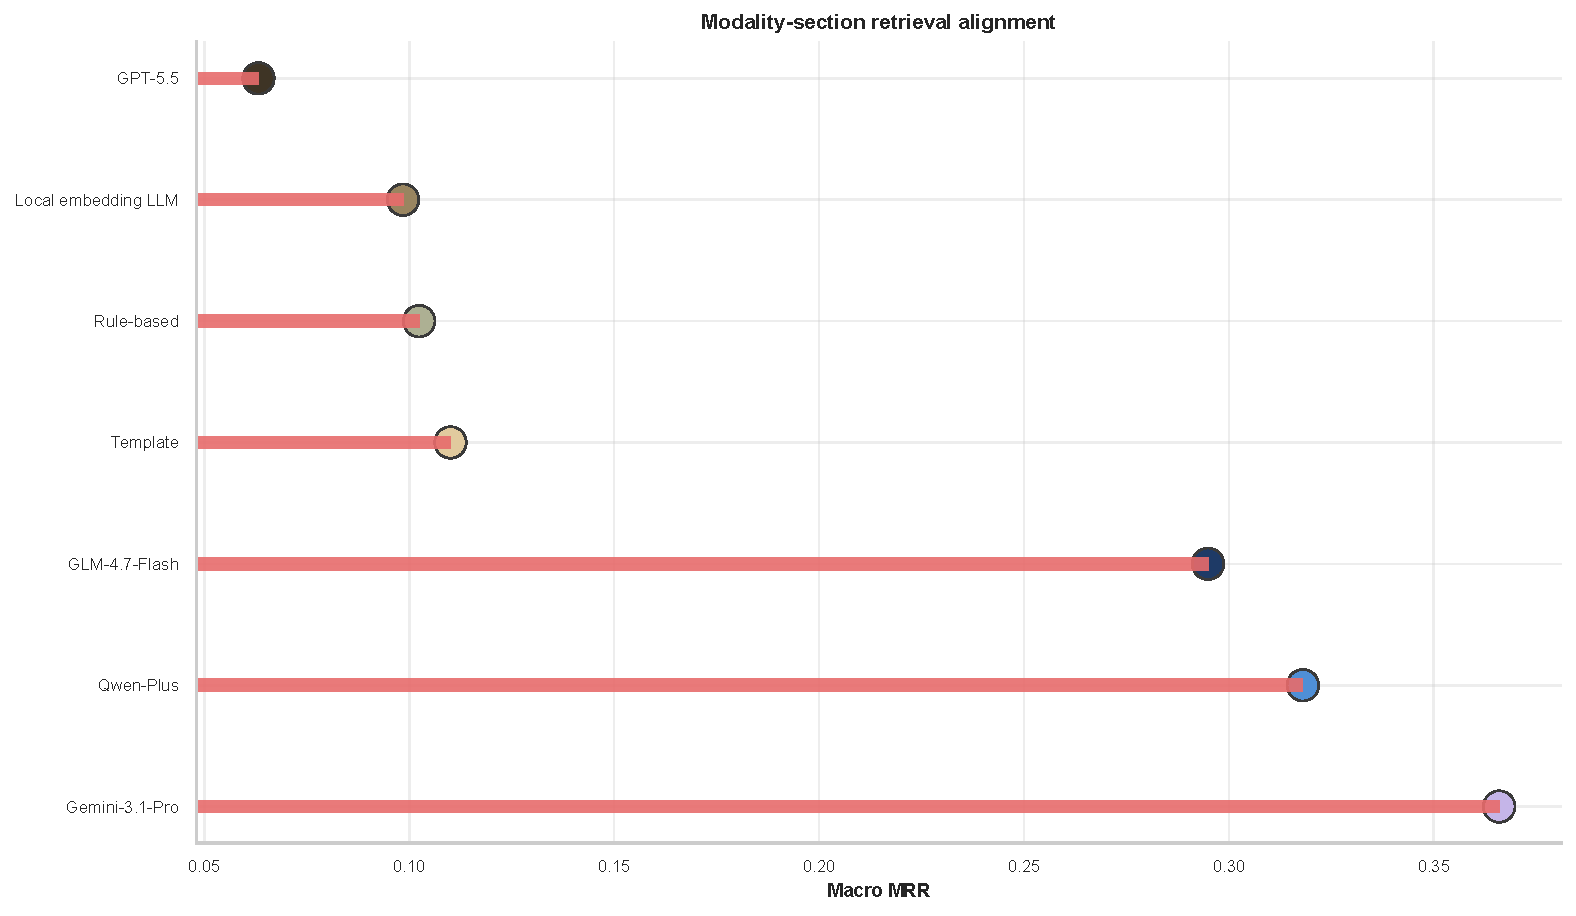
\includegraphics[width=\linewidth]{final_Fig/P5_stage2_macro_mrr.pdf}
%   \hfill
%   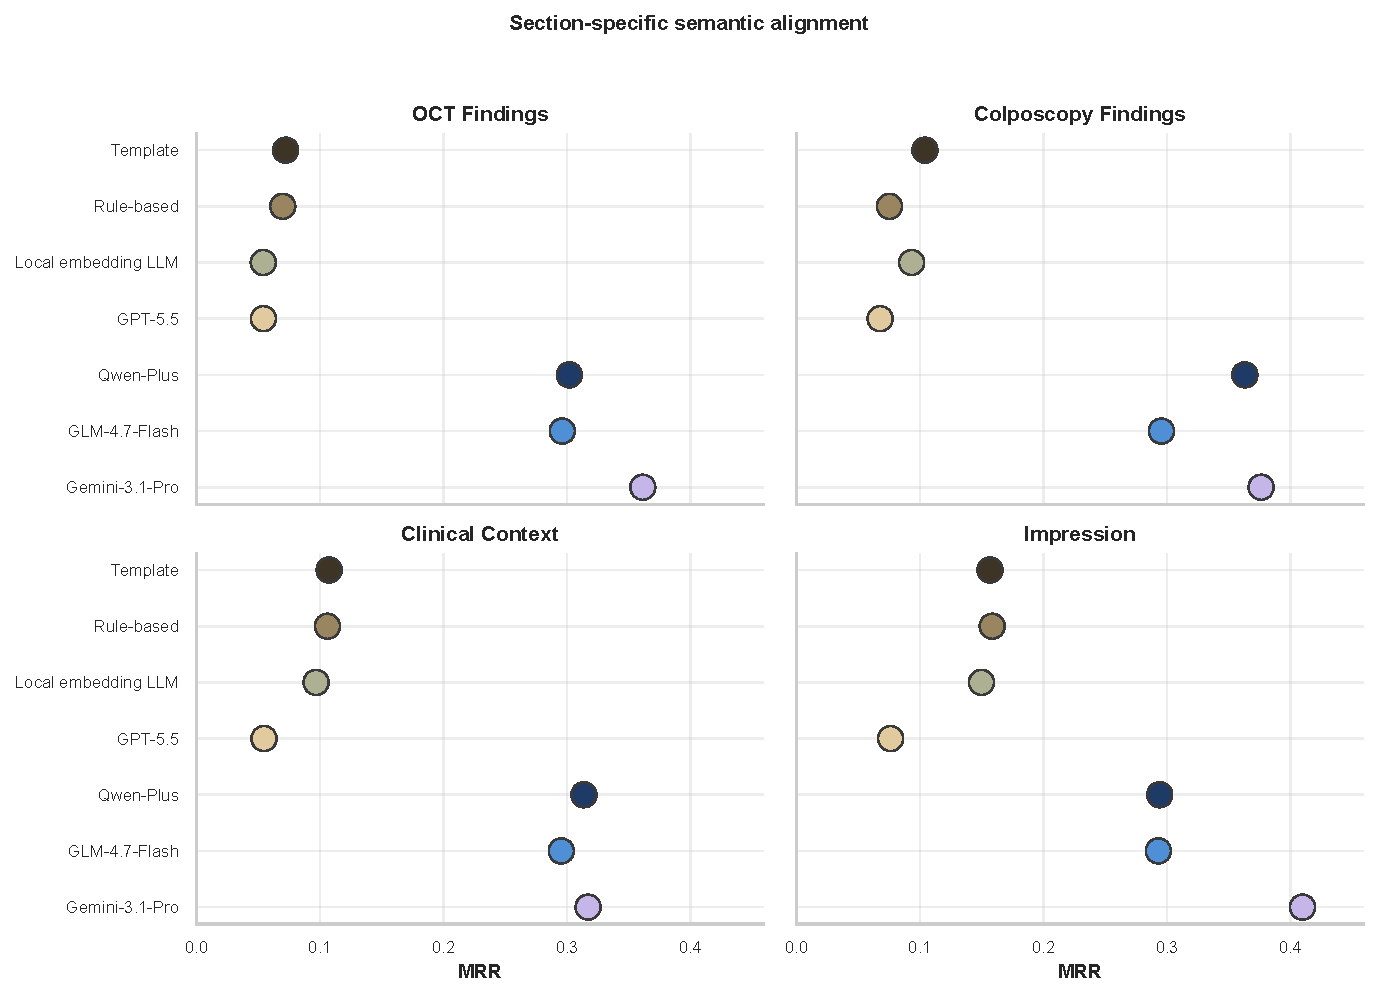
\includegraphics[width=\linewidth]{final_Fig/P6_stage2_section_mrr.pdf}
%   \caption{Supplementary Stage 2 alignment evaluation for provider-generated pseudo reports. Macro MRR and section-specific MRR quantify how well report sections generated by different sources support modality-section semantic retrieval.}
%   \label{app:fig:api_alignment_mrr}
% \end{figure}

% \subsection{Section-specific retrieval performance across providers}
% \label{app:subsec:api_section_mrr}
% \begin{figure}[!htbp]
%   \centering
%   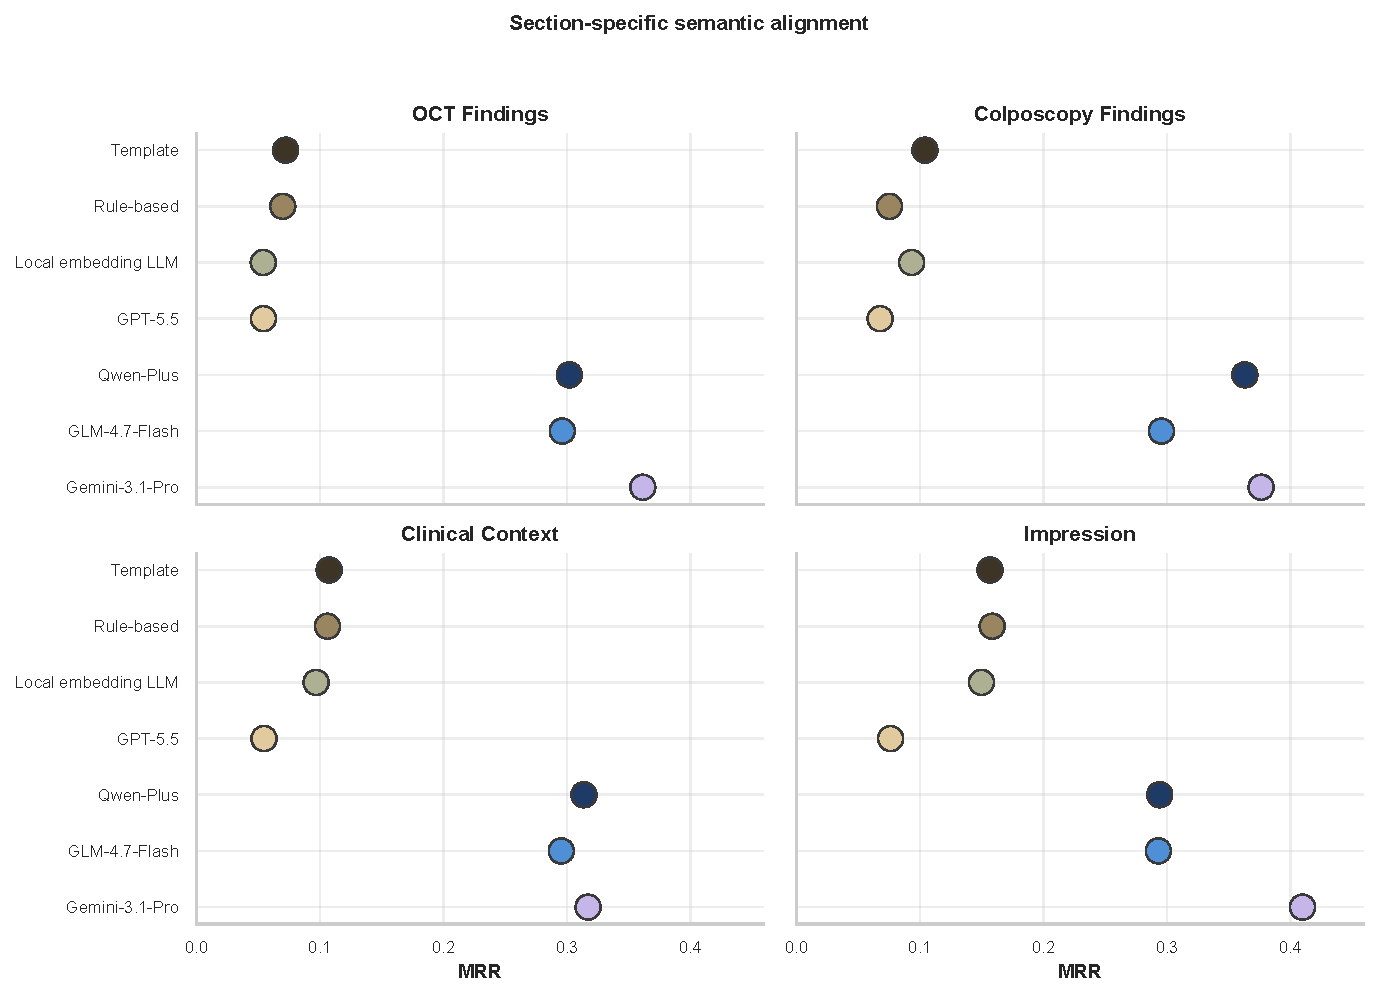
\includegraphics[width=\linewidth]{final_Fig/P6_stage2_section_mrr.pdf}
%   \caption{Supplementary section-specific retrieval performance across pseudo-report providers. The analysis separately evaluates alignment for OCT findings, colposcopy findings, clinical context, and impression sections.}
%   \label{app:fig:api_section_mrr}
% \end{figure}

% \subsection{Downstream scarcity surrogate for API-generated pseudo reports}
% \label{app:subsec:api_downstream_scarcity}
% \begin{figure}[!htbp]
%   \centering
%   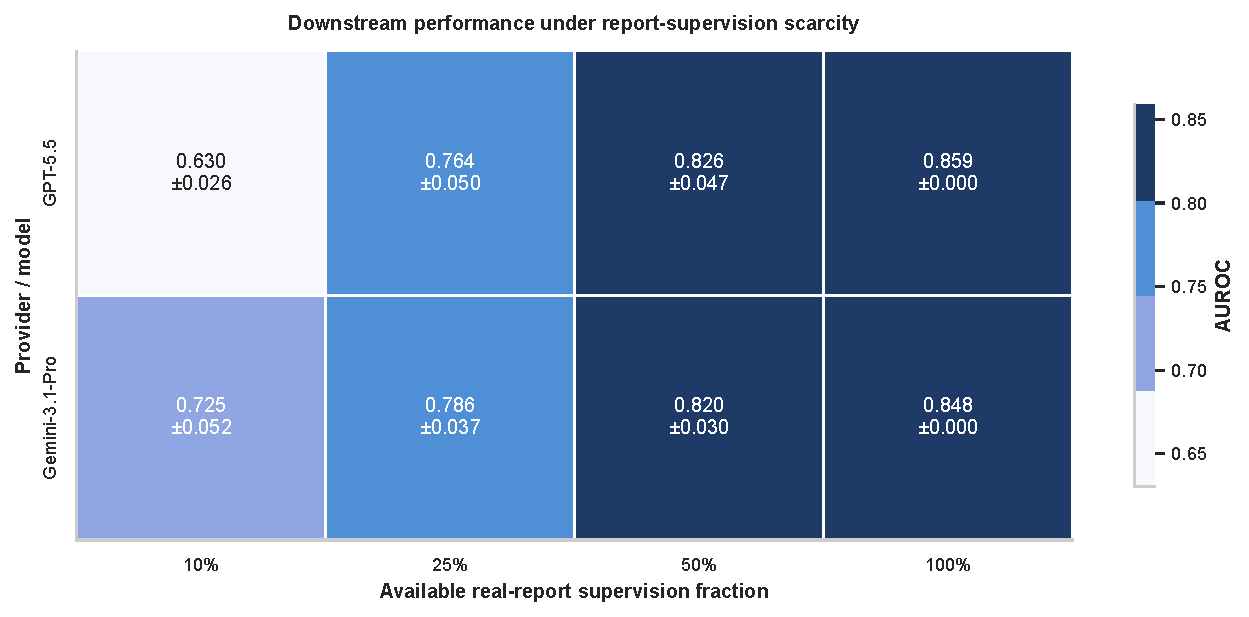
\includegraphics[width=\linewidth]{final_Fig/P7_stage3_scarcity_auc.pdf}
%   \caption{Supplementary Stage 3 downstream scarcity surrogate using selected API-generated pseudo reports. The figure compares performance under reduced real-report supervision and evaluates whether externally generated structured reports provide useful supervision in low-report regimes.}
%   \label{app:fig:api_scarcity_auc}
% \end{figure}

% \subsection{Protocol harmonisation for pre-retrieval backbone results}
% \label{app:subsec:protocol_harmonisation_table}
% \begin{table*}[!htbp]
%   \centering
%   \caption{Supplementary protocol-harmonisation table. Pre-retrieval-calibration held-out test performance at validation-selected thresholds.}
%   \label{app:tab:main_comparison}
%   \scriptsize
%   \begin{threeparttable}
%   \resizebox{\linewidth}{!}{%
%   \begin{tabular}{lrrr}
%     \toprule
%     \textbf{Model} & \textbf{AUROC [95\% CI]} & \textbf{F1 [95\% CI]} & \textbf{Threshold} \\
%     \midrule
%     \textbf{MOSAIC-RASA backbone} & \textbf{0.832} [0.757, 0.897] & \textbf{0.611} [0.458, 0.737] & 0.37 \\
%     LCAD w/o section alignment     & \underline{0.826} [0.749, 0.894] & 0.510 [0.381, 0.624] & 0.24 \\
%     Pseudo-augmented LCAD          & \underline{0.826} [0.747, 0.894] & \underline{0.545} [0.395, 0.674] & 0.39 \\
%     Fusion w/o report anchor       & 0.802 [0.726, 0.873] & 0.457 [0.344, 0.557] & 0.16 \\
%     Image-only report generator    & 0.763 [0.685, 0.837] & 0.453 [0.339, 0.553] & 0.17 \\
%     Real-report only               & 0.725 [0.640, 0.801] & 0.356 [0.263, 0.438] & 0.14 \\
%     Simple concatenation fusion    & 0.672 [0.584, 0.763] & 0.465 [0.380, 0.550] & 0.05 \\
%     Instruction-only report generator & 0.630 [0.547, 0.717] & 0.459 [0.394, 0.519] & 0.14 \\
%     \bottomrule
%   \end{tabular}%
%   }
%   \begin{tablenotes}[flushleft]
%     \footnotesize
%     \item All models were evaluated on the same locked held-out test set ($n=288$). The repeated $n$ column was removed and reported here.
%   \end{tablenotes}
%   \end{threeparttable}
% \end{table*}

% \subsection{MOSAIC metric profile for retrieval-calibrated fusion}
% \label{app:subsec:mosaic_metric_profile}
% \begin{figure}[!htbp]
%   \centering
%   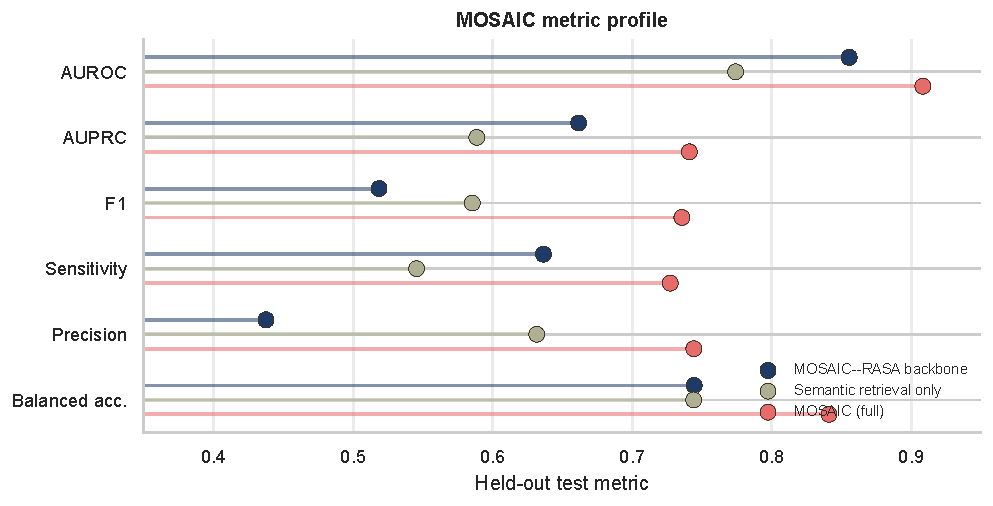
\includegraphics[width=\linewidth]{final_Fig/Figure_mosaic_metrics_heatmap.pdf}
%   \caption{Supplementary compact metric heatmap for MOSAIC. The heatmap compares the MOSAIC-RASA backbone, retrieval-only semantic priors, and MOSAIC across discrimination and threshold-dependent metrics.}
%   \label{app:fig:mosaic_metrics_heatmap}
% \end{figure}

% \subsection{Historical report-aware backbone AUROC comparison}
% \label{app:subsec:historical_main_auc}
% \begin{figure}[!htbp]
%   \centering
%   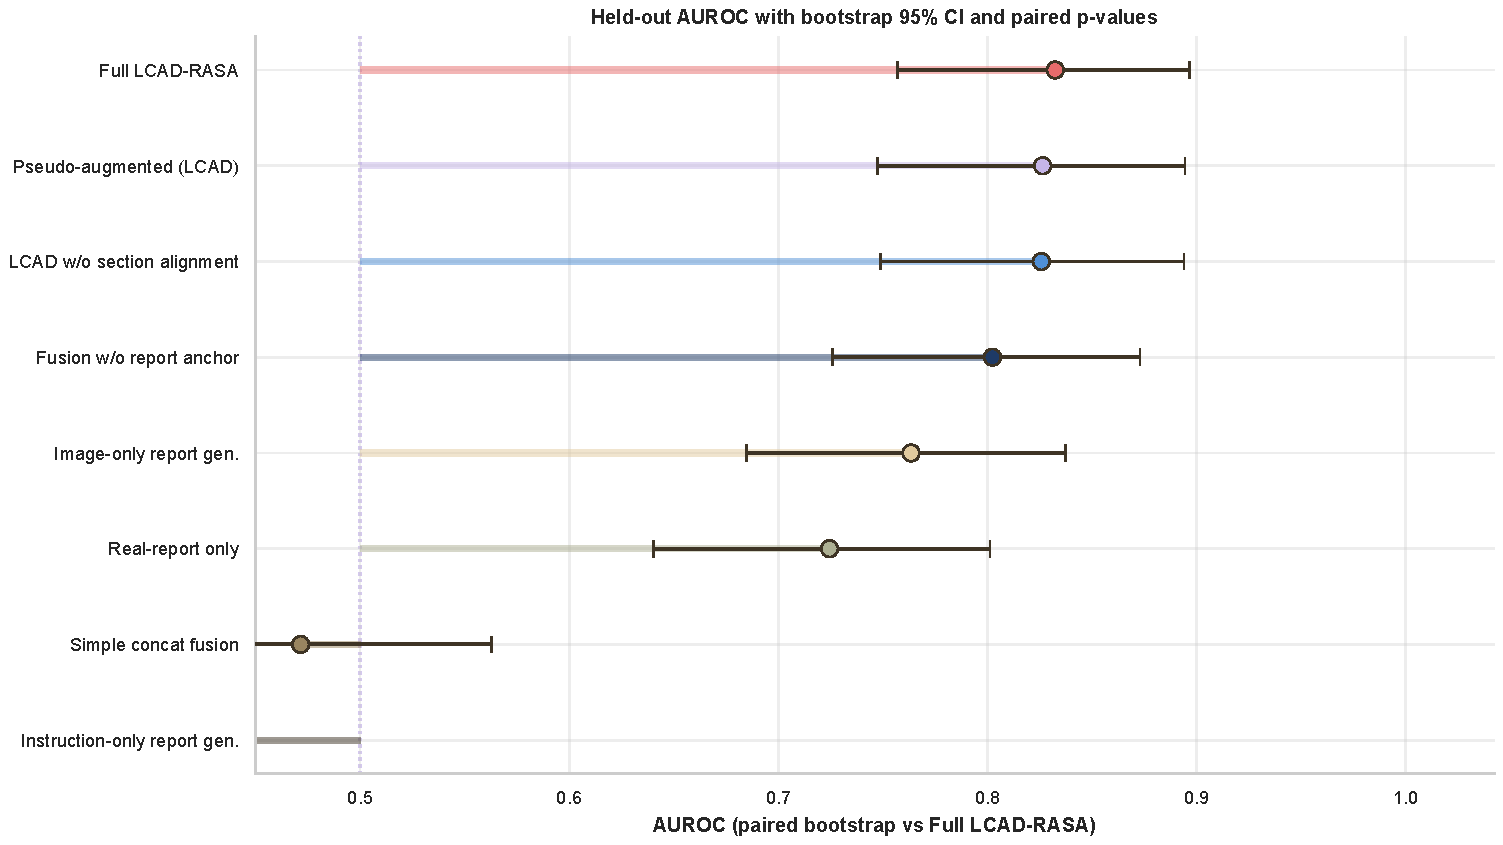
\includegraphics[width=\linewidth]{final_Fig/Figure_main_AUC_pointplot.pdf}
%   \caption{Supplementary protocol-harmonisation plot. Held-out AUROC of report-aware backbone variants under the locked retrospective protocol. Points indicate test-set AUROC and intervals denote bootstrap 95\% confidence intervals.}
%   \label{app:fig:main_auc}
% \end{figure}

% \subsection{Multi-metric profile of historical backbone variants}
% \label{app:subsec:historical_main_metrics}
% \begin{figure}[!htbp]
%   \centering
%   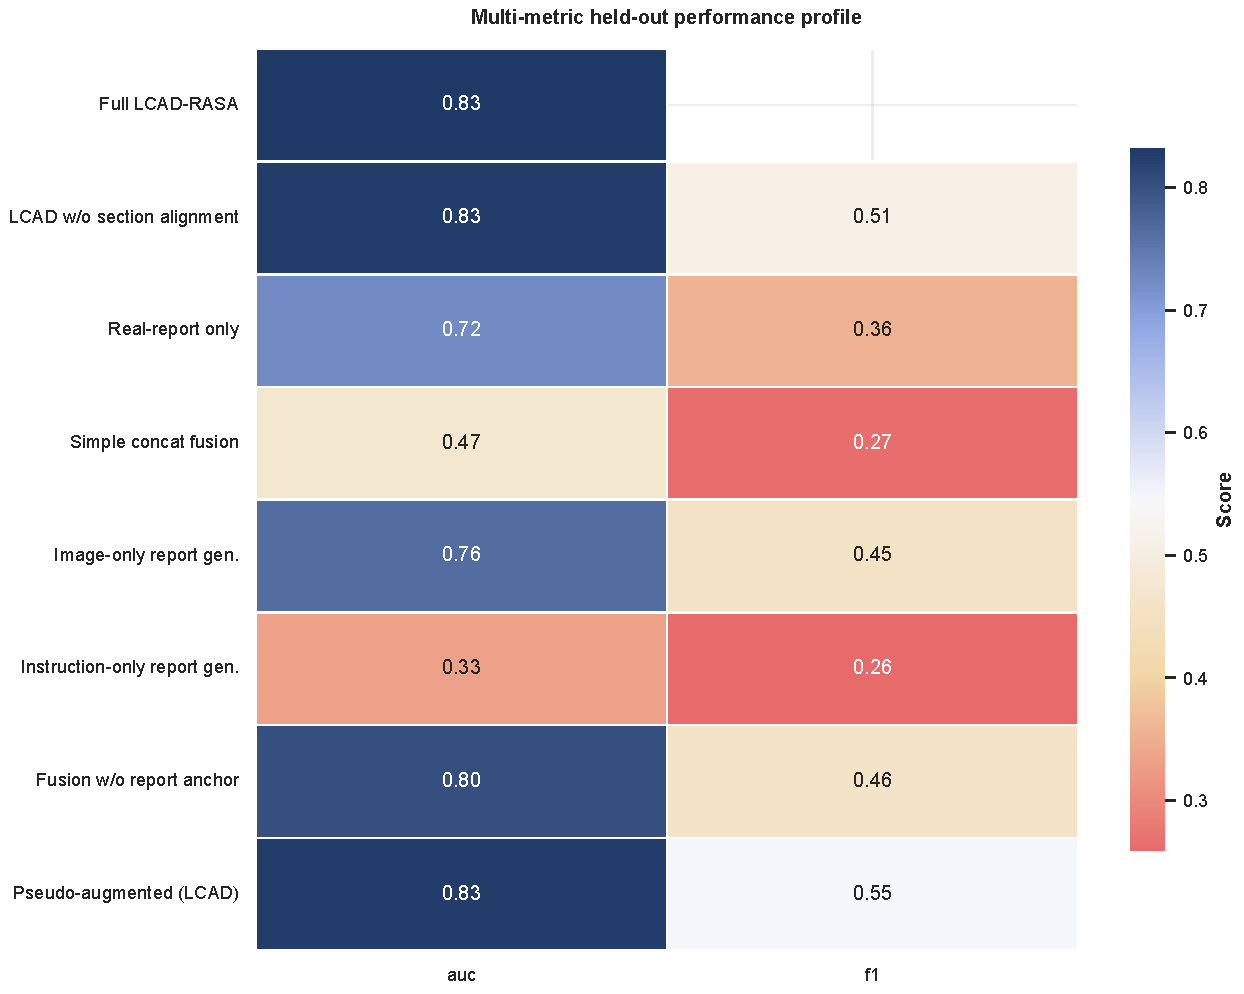
\includegraphics[width=\linewidth]{final_Fig/Figure_main_metrics_heatmap.pdf}
%   \caption{Supplementary multi-metric held-out performance profile across historical backbone variants. The heatmap summarises discrimination, threshold-dependent performance, report consistency, and related evaluation metrics under the same locked test protocol.}
%   \label{app:fig:main_metrics}
% \end{figure}

% \subsection{AUROC--F1 trade-off among backbone variants}
% \label{app:subsec:auc_f1_tradeoff}
% \begin{figure}[!htbp]
%   \centering
%   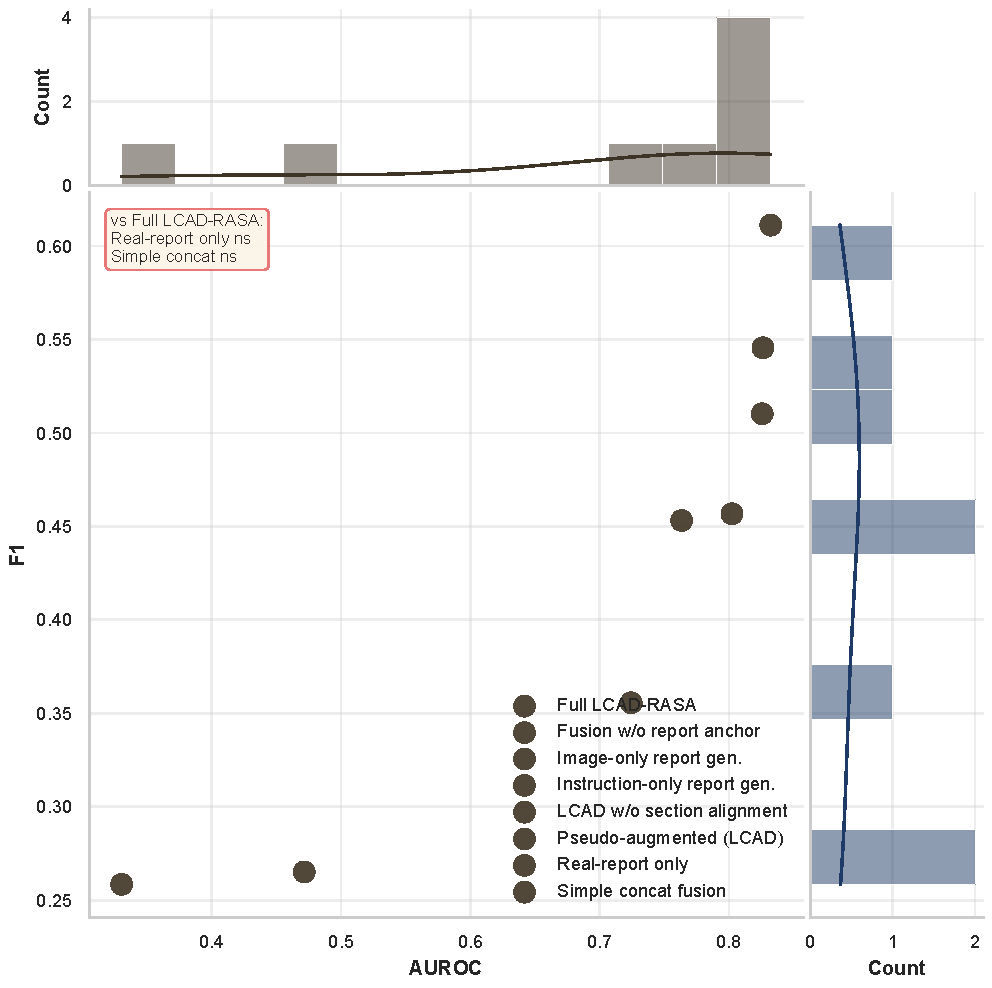
\includegraphics[width=\linewidth]{final_Fig/Figure_main_auc_f1_scatter.pdf}
%   \caption{Supplementary AUROC--F1 operating trade-off across historical backbone variants. The scatter plot contrasts rank-based discrimination with threshold-dependent classification performance on the held-out test set.}
%   \label{app:fig:main_auc_f1}
% \end{figure}

% \subsection{LLM-specific semantic-tag availability and retrieval ablation}
% \label{app:subsec:llm_tag_availability}
% \begin{table*}[!htbp]
%   \centering
%   \caption{Supplementary Table S4a. LLM-specific semantic-tag and retrieval ablation.}
%   \label{app:tab:llm_specific_ablation}
%   \scriptsize
%   \begin{threeparttable}
%   \resizebox{\linewidth}{!}{%
%   \begin{tabular}{lcccrrrrrrr}
%     \toprule
%     \textbf{Method} & \textbf{Uses LLM} & \textbf{\makecell{Train-only\\bank}} & \textbf{\makecell{Validation\\fusion}} & \textbf{AUROC} & \textbf{AUPRC} & \textbf{F1} & \textbf{Sensitivity} & \textbf{Specificity} & \textbf{$\alpha$} & \textbf{Threshold} \\
%     \midrule
%     MOSAIC-RASA backbone only & No & \NA & Threshold only & 0.856 & 0.662 & 0.519 & 0.636 & 0.852 & \NA & 0.39 \\
%     Clean rule-tag retrieval only & No & Yes & Threshold only & 0.724 & 0.349 & 0.480 & 0.682 & 0.791 & \NA & 0.30 \\
%     MOSAIC-Tag: RASA + clean rule-tag fusion & No & Yes & Yes & 0.878 & 0.695 & 0.556 & 0.568 & 0.914 & 0.10 & 0.40 \\
%     LLM-tag retrieval only & Yes & Yes & Threshold only & \NA & \NA & \NA & \NA & \NA & \NA & \NA \\
%     RASA + LLM-tag retrieval fusion & Yes & Yes & Yes & \NA & \NA & \NA & \NA & \NA & \NA & \NA \\
%     RASA + LLM-tag fusion + verifier weighting & Yes & Yes & Yes & \NA & \NA & \NA & \NA & \NA & \NA & \NA \\
%     MOSAIC & Indirect & Yes & Yes & 0.908 & 0.741 & 0.736 & 0.727 & 0.955 & \NA & 0.50 \\
%     CLIP-style contrastive baseline & No & \NA & Threshold only & 0.888 & 0.739 & 0.640 & 0.545 & 0.971 & \NA & 0.79 \\
%     \bottomrule
%   \end{tabular}%
%   }
%   \begin{tablenotes}[flushleft]
%     \footnotesize
%     \item LLM-tag rows are unavailable because no valid LLM semantic tag table was generated in the current run. Rule-tag rows are deterministic fallback audits and must not be interpreted as LLM evidence. All available tag-retrieval rows used a cleaned training-only bank; fusion weights and thresholds were selected on validation data only. MOSAIC-Tag is a secondary semantic-tag audit rather than the primary MOSAIC model.
%   \end{tablenotes}
%   \end{threeparttable}
% \end{table*}

% \subsection{Cleaned semantic-tag source ablations and negative controls}
% \label{app:subsec:semantic_tag_controls}
% \begin{table*}[!htbp]
%   \centering
%   \caption{Supplementary Table S4b. Cleaned semantic-tag source ablation and negative controls.}
%   \label{app:tab:semantic_tag_source_ablation_cleaned}
%   \scriptsize
%   \begin{threeparttable}
%   \resizebox{\linewidth}{!}{%
%   \begin{tabular}{lrrrrp{4.2cm}}
%     \toprule
%     \textbf{Variant} & \textbf{\makecell{Retrieval-only\\AUROC}} & \textbf{\makecell{Fusion\\AUROC}} & \textbf{\(\Delta\)AUROC vs RASA} & \textbf{\makecell{95\% interval}} & \textbf{Interpretation} \\
%     \midrule
%     MOSAIC-Tag, all clean rule tags & 0.724 & 0.878 & 0.023 & 0.003--0.042 & Cleaned semantic-tag audit; secondary analysis \\
%     No impression tags & 0.724 & 0.878 & 0.023 & 0.003--0.042 & No loss after removing impression-tag column \\
%     No severity tags & 0.724 & 0.878 & 0.023 & 0.003--0.042 & No loss after removing severity-tag column \\
%     No diagnostic terminology & 0.724 & 0.878 & 0.023 & 0.003--0.042 & Effect persisted after diagnostic-term removal \\
%     Modality-only or visual-only tags & 0.500 & 0.856 & 0.000 & 0.000--0.000 & Collapsed to MOSAIC-RASA backbone \\
%     Train-label prior only & 0.500 & 0.856 & 0.000 & 0.000--0.000 & Negative control did not improve over backbone \\
%     Random tag query & 0.462 & 0.853 & -0.002 & -0.006--0.002 & Random-query negative control removed the tag gain \\
%     Random train-label bank & 0.582 & 0.856 & 0.000 & 0.000--0.000 & Label-permutation control removed the tag gain \\
%     Same-centre excluded retrieval & 0.628 & 0.864 & 0.008 & -0.003--0.019 & Cross-centre retrieval retained limited signal but was weaker \\
%     \bottomrule
%   \end{tabular}%
%   }
%   \begin{tablenotes}[flushleft]
%     \footnotesize
%     \item All rows used the semantic-tag audit protocol: cleaned tag input, training-only tag bank, validation-selected fusion weight and threshold, and locked held-out test metrics. MOSAIC-Tag passed leakage screening and negative controls, but its role is a lightweight semantic-prior audit rather than a replacement for MOSAIC.
%   \end{tablenotes}
%   \end{threeparttable}
% \end{table*}

% \subsection{RASA alignment-weight sensitivity}
% \label{app:subsec:rasa_lambda_sweep}
% \begin{table}[!htbp]
%   \centering
%   \caption{Supplementary Table S1. RASA alignment-weight sweep.}
%   \label{app:tab:s1_rasa_lambda_align_sweep}
%   \small
%   \begin{threeparttable}
%   \begin{tabular}{lr}
%     \toprule
%     \textbf{$\lambda_{\mathrm{align}}$} & \textbf{AUROC} \\
%     \midrule
%     0.00 & 0.766 \\
%     0.01 & 0.766 \\
%     0.05 & 0.769 \\
%     0.10 & 0.773 \\
%     0.20 & \textbf{0.776} \\
%     0.50 & 0.772 \\
%     1.00 & 0.764 \\
%     \bottomrule
%   \end{tabular}
%   \begin{tablenotes}[flushleft]
%     \footnotesize
%     \item F1 was 0.451, label consistency was 0.641, and section completeness was 1.000 for all settings; these constant columns were omitted.
%   \end{tablenotes}
%   \end{threeparttable}
% \end{table}

% \subsection{Input-modality ablation}
% \label{app:subsec:modality_ablation}
% \begin{table*}[!htbp]
%   \centering
%   \caption{Supplementary Table S3. Modality ablation.}
%   \label{app:tab:s3_modality_ablation}
%   \small
%   \begin{threeparttable}
%   \resizebox{\linewidth}{!}{%
%   \begin{tabular}{lrrrr}
%     \toprule
%     \textbf{Variant} & \textbf{AUROC} & \textbf{F1} & \textbf{Sensitivity} & \textbf{Specificity} \\
%     \midrule
%     Colposcopy + clinical instruction        & \textbf{0.850} & 0.524 & \underline{0.614} & 0.869 \\
%     Full without fused visual embedding      & \underline{0.840} & \underline{0.571} & 0.500 & \textbf{0.955} \\
%     OCT + colposcopy + clinical instruction  & \underline{0.840} & \underline{0.571} & 0.500 & \textbf{0.955} \\
%     Colposcopy only                          & 0.838 & \textbf{0.581} & \underline{0.614} & 0.910 \\
%     Full with fused visual embedding         & 0.836 & 0.561 & 0.523 & 0.939 \\
%     OCT + colposcopy                         & 0.826 & 0.543 & 0.568 & 0.906 \\
%     OCT + clinical instruction               & 0.765 & 0.466 & 0.386 & \underline{0.951} \\
%     OCT only                                 & 0.740 & 0.353 & 0.409 & 0.836 \\
%     Clinical instruction only                & 0.683 & 0.441 & \textbf{0.727} & 0.717 \\
%     \bottomrule
%   \end{tabular}%
%   }
%   \begin{tablenotes}[flushleft]
%     \footnotesize
%     \item Label consistency was 0.641 for all modality variants and was removed as a constant column.
%   \end{tablenotes}
%   \end{threeparttable}
% \end{table*}

% \subsection{LCAD pseudo-report quality-control ablation}
% \label{app:subsec:lcad_qc_ablation}
% \begin{table}[!htbp]
%   \centering
%   \caption{Supplementary Table S4. LCAD pseudo-report quality-control ablation.}
%   \label{app:tab:s4_lcad_qc_ablation}
%   \small
%   \begin{threeparttable}
%   \begin{tabular}{lrrrr}
%     \toprule
%     \textbf{QC strategy} & \textbf{AUROC} & \textbf{F1} & \textbf{Sensitivity} & \textbf{Specificity} \\
%     \midrule
%     \makecell[l]{Pseudo reports, no QC;\\QC-pass pseudo reports only;\\QC-score weighting only;\\Pseudo confidence weighting only;\\QC-confidence weighted pseudo reports} & 0.836 & 0.561 & 0.523 & 0.939 \\
%     \bottomrule
%   \end{tabular}
%   \begin{tablenotes}[flushleft]
%     \footnotesize
%     \item All QC variants produced identical downstream metrics under this retrospective configuration. Duplicate rows were therefore merged. Label consistency was 0.641 for all variants.
%   \end{tablenotes}
%   \end{threeparttable}
% \end{table}

% \subsection{Failure-enriched pseudo-report QC stress test}
% \label{app:subsec:qc_stress_test}
% \begin{table}[!htbp]
%   \centering
%   \caption{Supplementary Table S4c. Failure-enriched QC stress-test v2 audit.}
%   \label{app:tab:qc_failure_stress_test}
%   \small
%   \begin{threeparttable}
%   \begin{tabular}{p{5.0cm}rp{5.2cm}}
%     \toprule
%     \textbf{Stress-test metric} & \textbf{Value} & \textbf{Interpretation} \\
%     \midrule
%     Clean pseudo-report QC pass rate & 1.000 & clean baseline retained \\
%     Corrupted pseudo-report QC pass rate & 0.742 & corrupted variants partly rejected or down-weighted \\
%     Mean QC score, clean vs corrupted & 1.000 vs 0.855 & corrupted reports down-weighted \\
%     Severe-error flag rate, clean vs corrupted & 0.000 vs 0.258 & severe failures enriched among corrupted reports \\
%     Contradiction detection rate & 1.000 & expected contradiction flags detected \\
%     Hallucination detection rate & 0.999 & unsupported terminology or missing-modality evidence detected \\
%     Missing-section detection rate & 1.000 & empty required sections detected \\
%     Modality-swap detection rate & 1.000 & v2 modality--section consistency detector captured OCT--colposcopy swaps and shuffled sections \\
%     Duplicate-template detection rate & 1.000 & repeated template text detected \\
%     \bottomrule
%   \end{tabular}
%   \begin{tablenotes}[flushleft]
%     \footnotesize
%     \item The stress test used all 1,153 pseudo-report candidates and the v2 QC function. The clean modality-swap false-positive rate was 0.000. No retraining under corrupted reports was performed, and no LLM verifier comparison is claimed. Source files: \texttt{outputs/qc/qc\_stress\_test\_v2.csv}, \texttt{outputs/qc/qc\_stress\_test\_v2\_detail.csv}, and \texttt{outputs/qc/qc\_failure\_enriched\_stress\_test.png}.
%   \end{tablenotes}
%   \end{threeparttable}
% \end{table}

% \subsection{RASA component ablation}
% \label{app:subsec:rasa_component_ablation}
% \begin{table*}[!htbp]
%   \centering
%   \caption{Supplementary Table S5. RASA component ablation.}
%   \label{app:tab:s5_rasa_component_ablation}
%   \small
%   \begin{threeparttable}
%   \resizebox{\linewidth}{!}{%
%   \begin{tabular}{lrrrr}
%     \toprule
%     \textbf{Variant} & \textbf{AUROC} & \textbf{F1} & \textbf{Sensitivity} & \textbf{Specificity} \\
%     \midrule
%     Risk-head auxiliary only                 & \textbf{0.838} & 0.538 & \underline{0.568} & 0.902 \\
%     No section alignment                     & \textbf{0.838} & 0.479 & \textbf{0.636} & 0.816 \\
%     No label-consistency loss                & 0.836 & \textbf{0.579} & 0.500 & \textbf{0.959} \\
%     MOSAIC-RASA backbone                    & 0.836 & \underline{0.561} & 0.523 & \underline{0.939} \\
%     \makecell[l]{No risk head;\\Report loss only;\\Section alignment auxiliary only} & 0.750 & 0.465 & 0.550 & 0.820 \\
%     \bottomrule
%   \end{tabular}%
%   }
%   \begin{tablenotes}[flushleft]
%     \footnotesize
%     \item Label consistency was 0.641 for all component variants and was removed as a constant column. Three variants with identical metrics were merged into one row.
%   \end{tablenotes}
%   \end{threeparttable}
% \end{table*}

% \subsection{Extended metric profiles for same-split baselines}
% \label{app:subsec:external_metric_profile}
% \begin{figure}[!htbp]
%   \centering
%   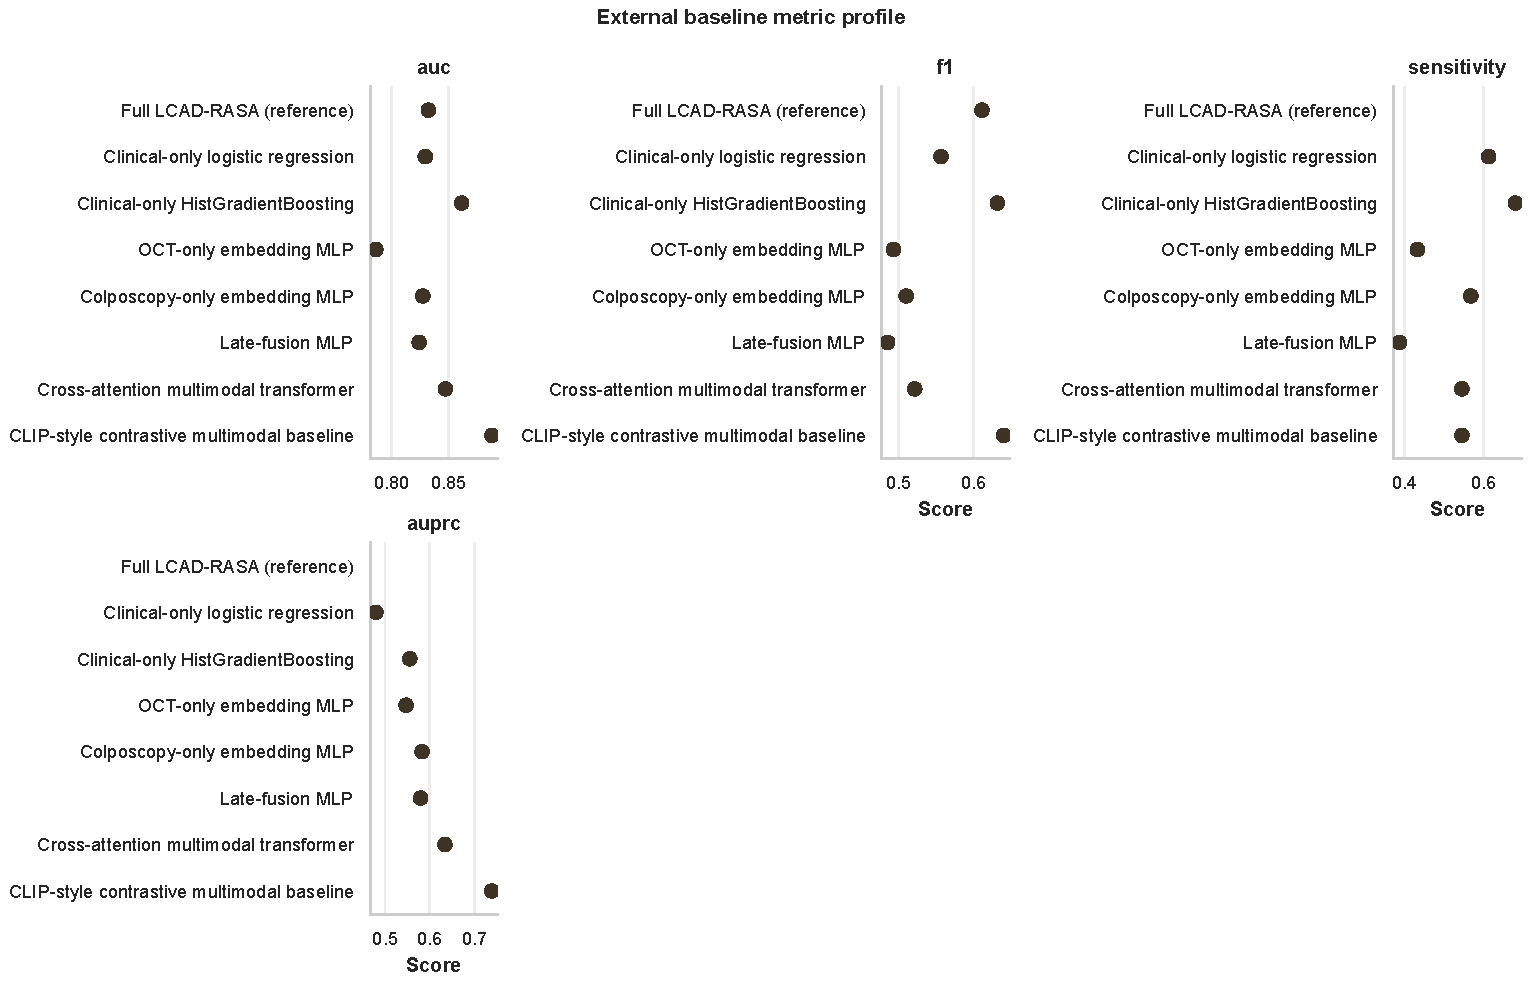
\includegraphics[width=\linewidth]{final_Fig/Figure_external_baselines_metric_dotplot.pdf}
%   \caption{Supplementary metric profile of MOSAIC, the MOSAIC-RASA backbone, and external baselines under the locked held-out protocol. The dot plot compares discrimination and threshold-dependent metrics across clinical-only, image-only, late-fusion, cross-attention, contrastive, and report-aware models.}
%   \label{app:fig:external_baselines_metrics}
% \end{figure}

% \subsection{Corrected paired-bootstrap recheck against the backbone}
% \label{app:subsec:external_pairwise_recheck}
% \begin{figure}[!htbp]
%   \centering
%   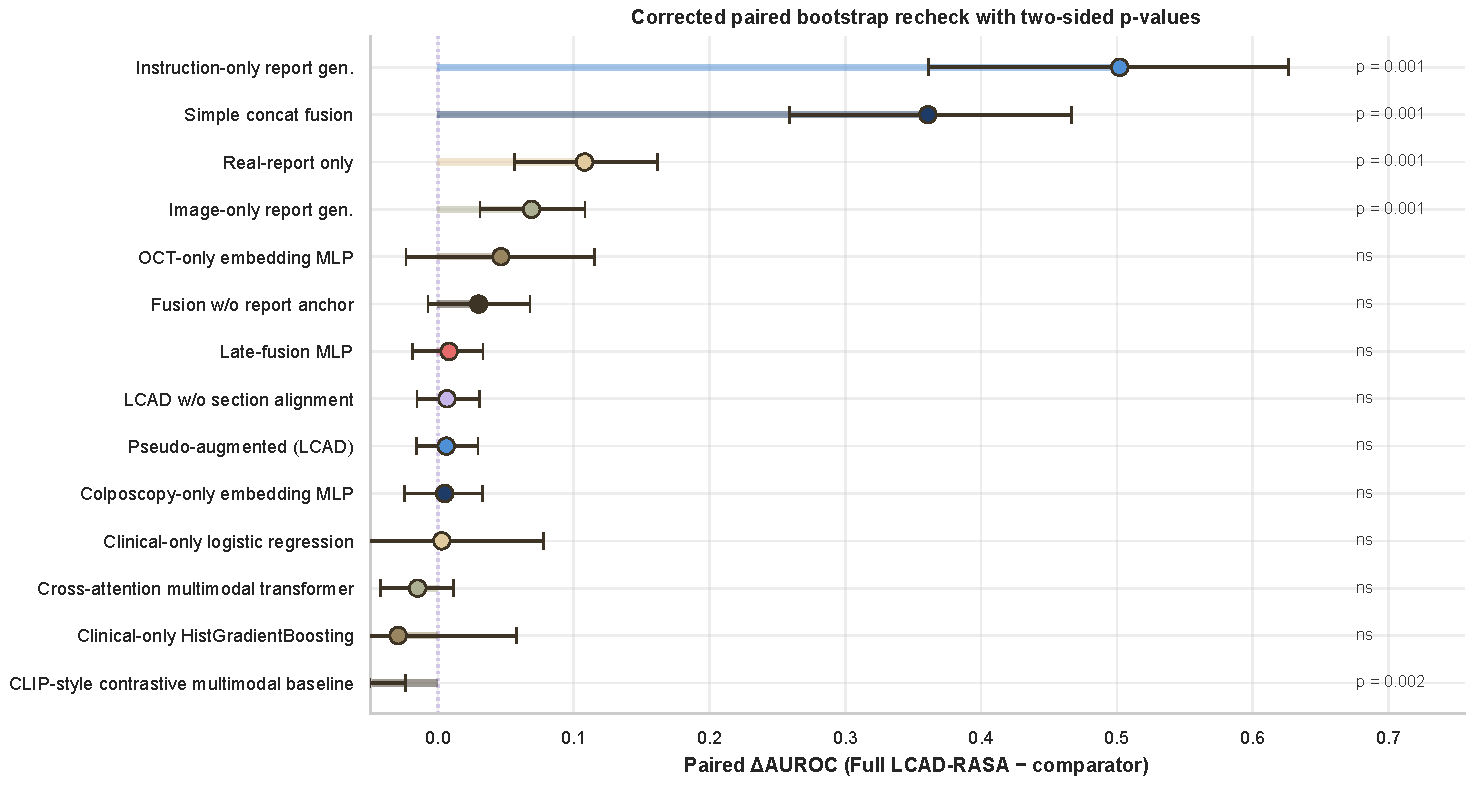
\includegraphics[width=\linewidth]{final_Fig/Figure_external_baselines_paired_delta_auc.pdf}
%   \caption{Supplementary corrected paired bootstrap AUROC differences relative to the MOSAIC-RASA backbone. Positive values favour the backbone, whereas negative values favour the comparator, with intervals estimated from paired test-set resampling.}
%   \label{app:fig:external_pairwise_recheck}
% \end{figure}

% \subsection{Alignment-weight sensitivity visualisation}
% \label{app:subsec:rasa_lambda_figure}
% \begin{figure}[!htbp]
%   \centering
%   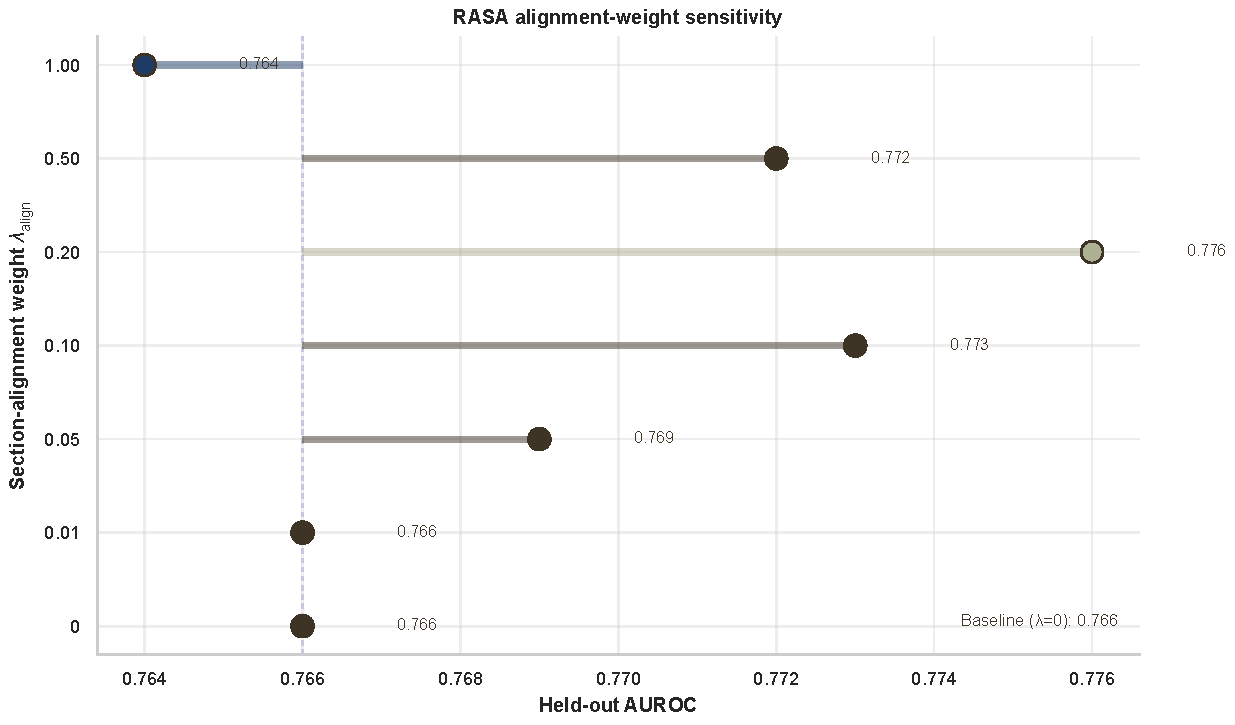
\includegraphics[width=\linewidth]{final_Fig/fig_rasa_lambda_lineplot.pdf}
%   \caption{Supplementary sensitivity of model performance to the RASA alignment weight. The sweep evaluates how varying the section-alignment loss weight affects downstream discrimination and report-related metrics.}
%   \label{app:fig:rasa_lambda}
% \end{figure}

% \subsection{Joint modality and RASA component visual ablations}
% \label{app:subsec:modality_component_figures}
% \begin{figure}[!htbp]
%   \centering
%   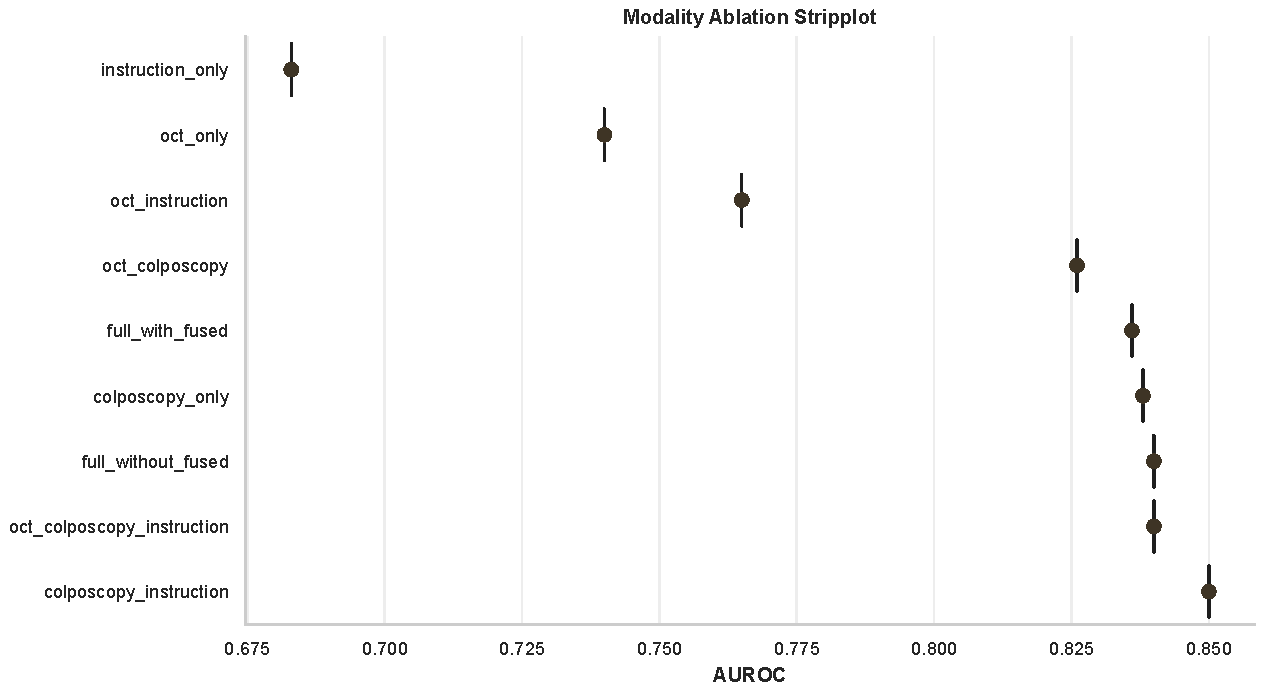
\includegraphics[width=\linewidth]{final_Fig/fig_modality_ablation_stripplot.pdf}
%   \hfill
%   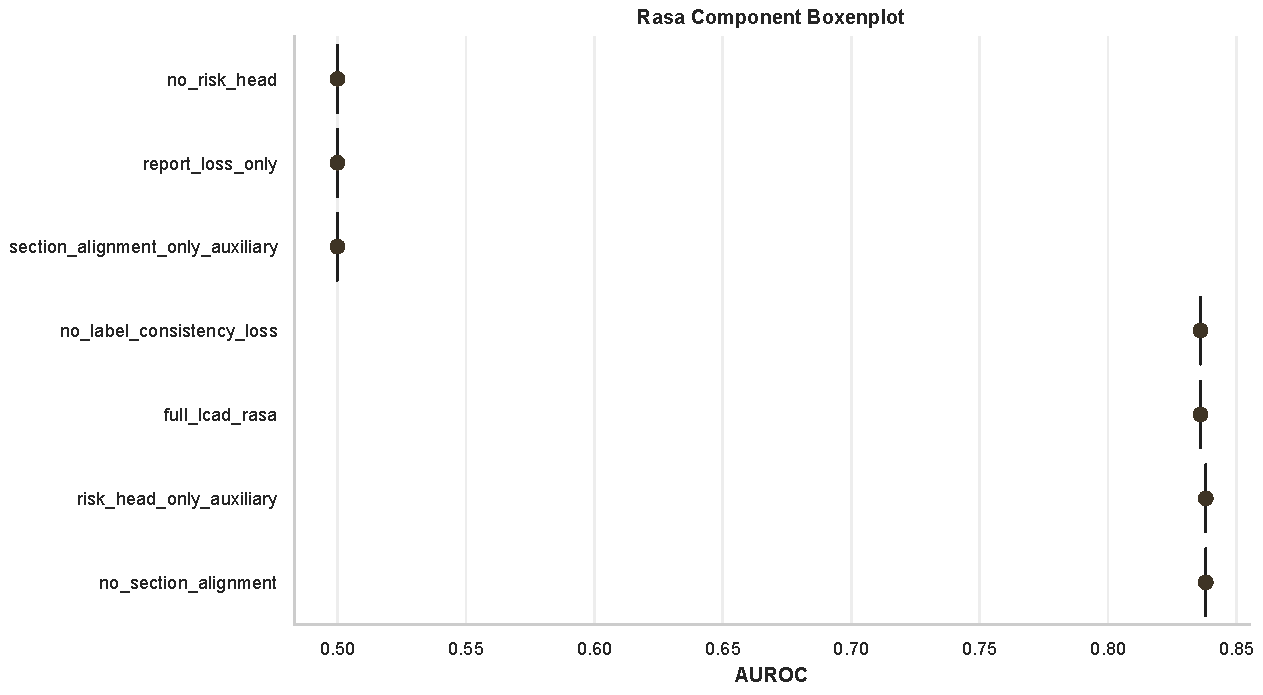
\includegraphics[width=\linewidth]{final_Fig/fig_rasa_component_boxenplot.pdf}
%   \caption{Supplementary ablation analysis of modality inputs and RASA components. The panels assess the contribution of OCT, colposcopy, clinical instruction, fused visual embeddings, section alignment, risk supervision, and label-consistency terms.}
%   \label{app:fig:rasa_component_boxenplot}
% \end{figure}

% \subsection{LCAD quality-control ablation visualisation}
% \label{app:subsec:qc_ablation_figure}
% \begin{figure}[!htbp]
%   \centering
%   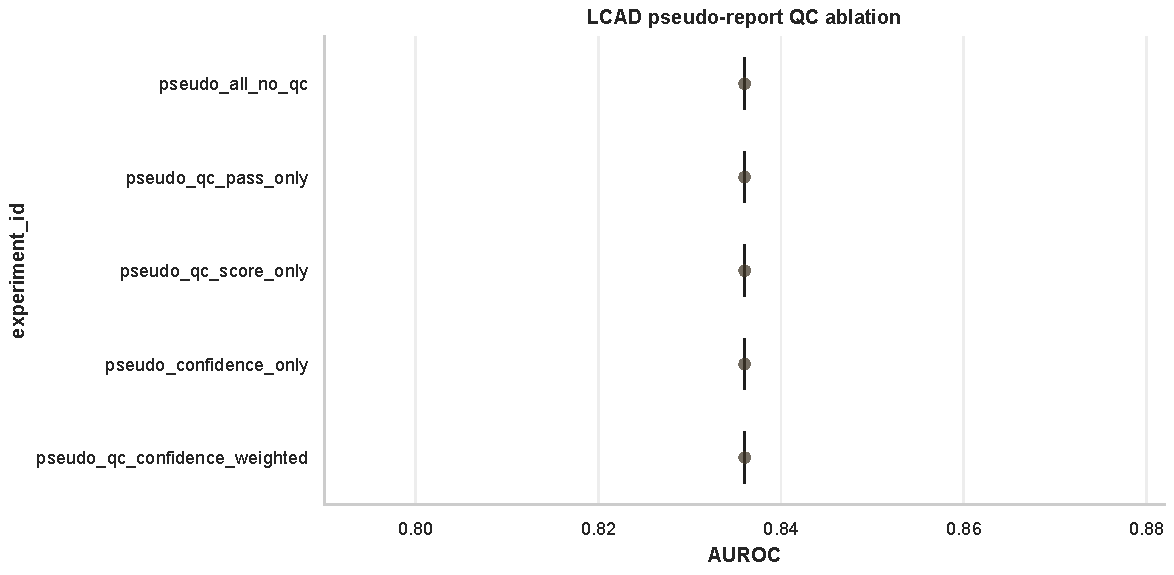
\includegraphics[width=0.82\linewidth]{final_Fig/fig_lcad_qc_ablation_barplot.pdf}
%   \caption{Supplementary quality-control ablation for LCAD pseudo-report supervision. The analysis evaluates whether alternative pseudo-report filtering and weighting strategies materially alter downstream performance under the retrospective configuration; the separate failure-enriched stress test evaluates report-safety flagging rather than AUROC change.}
%   \label{app:fig:qc_ablation}
% \end{figure}

% \subsection{Section-level perturbation degradation profiles}
% \label{app:subsec:perturbation_lineplot}
% \begin{figure}[!htbp]
%   \centering
%   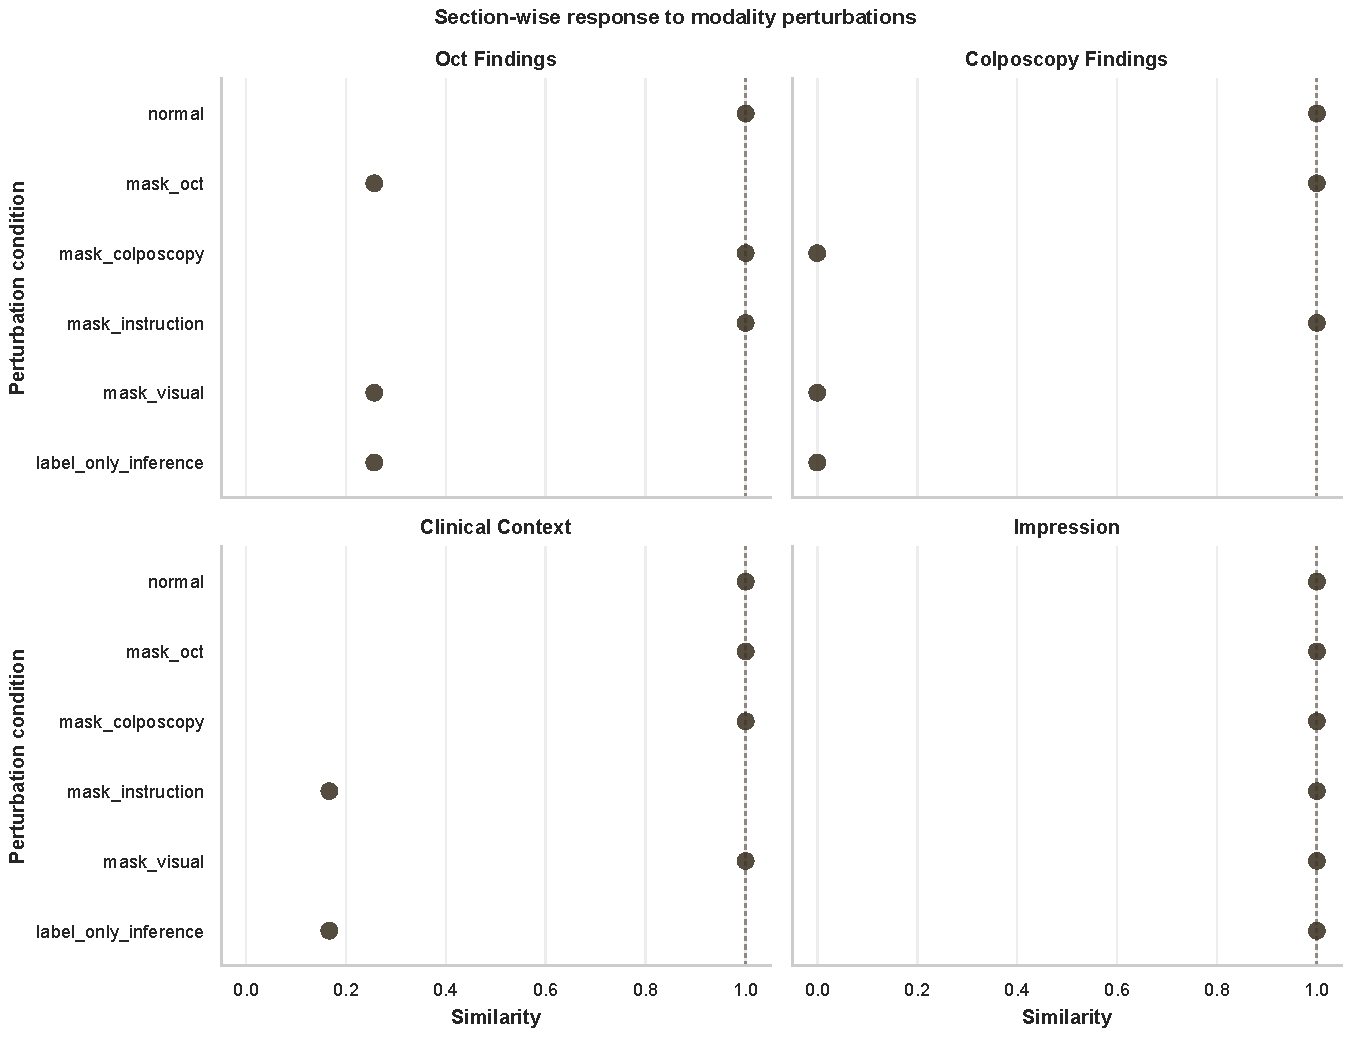
\includegraphics[width=\linewidth]{final_Fig/Figure3_modality_perturbation_lineplot.pdf}
%   \caption{Supplementary section-level degradation profiles following modality-specific perturbations. The curves show whether disruption of a given input modality preferentially degrades the report section that should be grounded in that modality.}
%   \label{app:fig:perturbation_lineplot}
% \end{figure}

% \subsection{Risk-score displacement under perturbation}
% \label{app:subsec:risk_delta}
% \begin{figure}[!htbp]
%   \centering
%   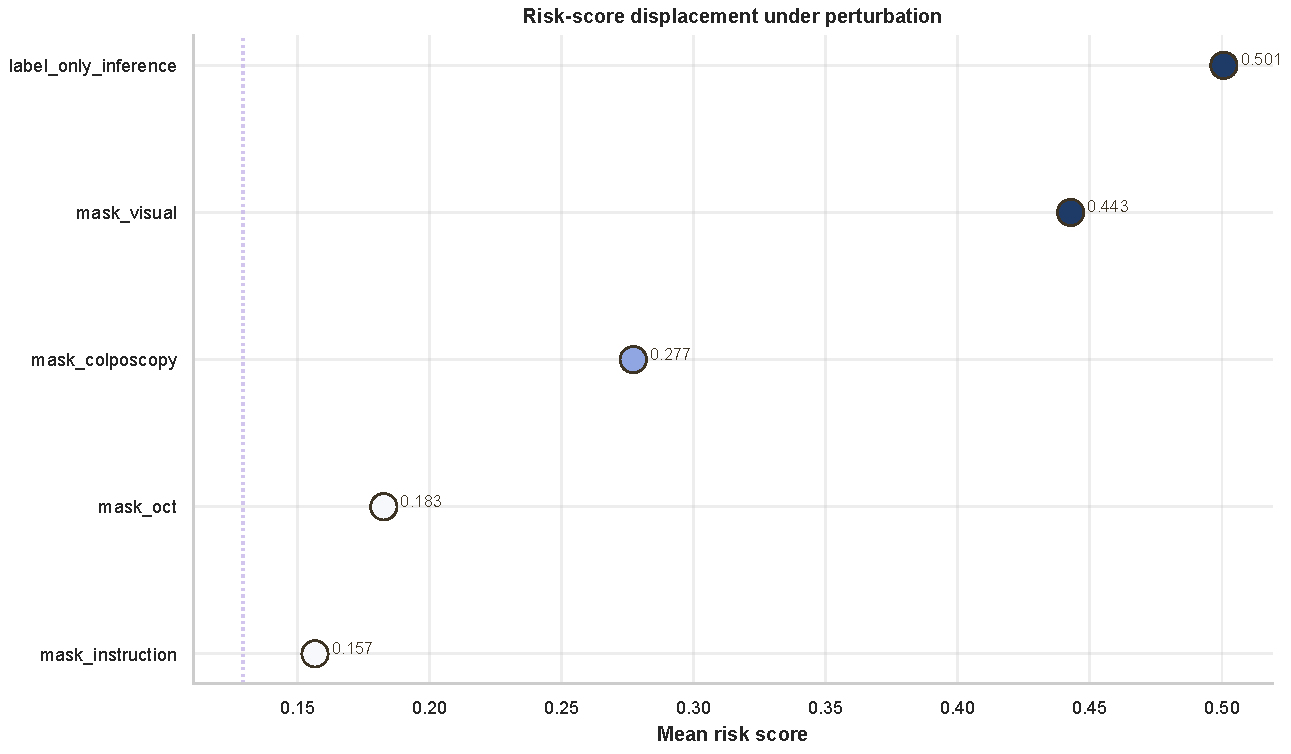
\includegraphics[width=\linewidth]{final_Fig/Figure3_risk_delta_stripplot.pdf}
%   \caption{Supplementary risk-score sensitivity to report-generation perturbations. Absolute changes in predicted risk quantify the extent to which modality masking, modality shuffling, and label-only inference alter the model's diagnostic output.}
%   \label{app:fig:risk_delta}
% \end{figure}

% \subsection{Expanded perturbation sensitivity matrix}
% \label{app:subsec:theme1_perturbation}
% \begin{figure}[!htbp]
%   \centering
%   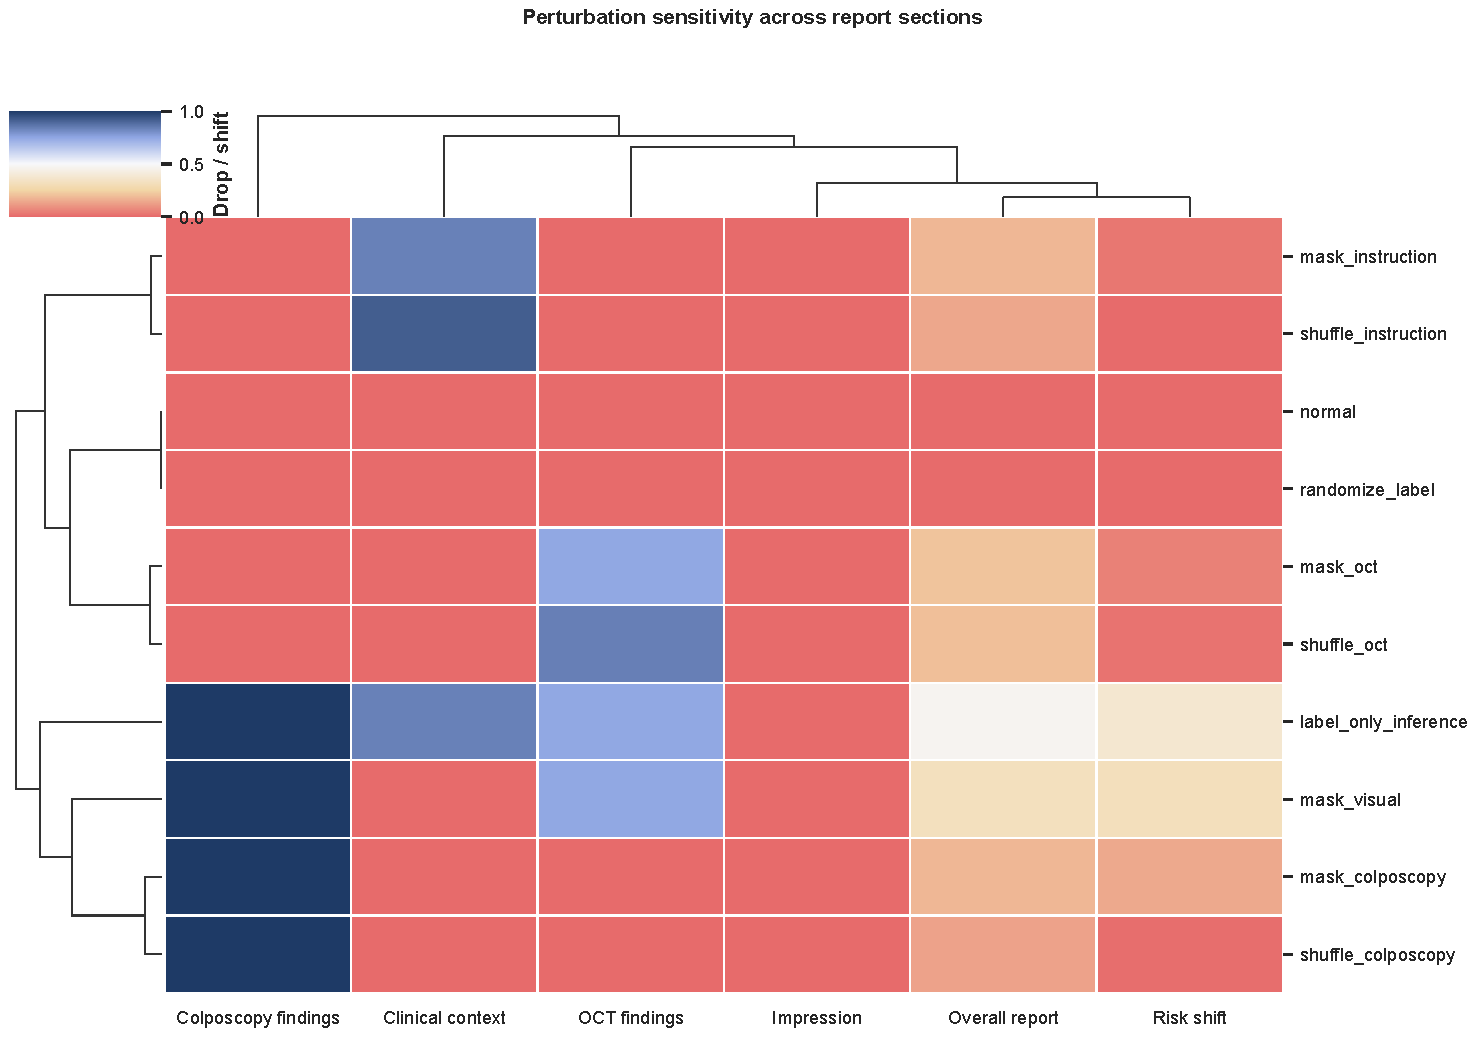
\includegraphics[width=\linewidth]{final_Fig/Figure_theme1_perturbation_sensitivity_matrix.pdf}
%   \caption{Supplementary upgraded perturbation sensitivity matrix for Theme 1 cross-modal semantic alignment. The matrix consolidates section-level degradation, report-level degradation, risk shift, and specificity of the expected modality-section response.}
%   \label{app:fig:theme1_perturbation}
% \end{figure}

% \subsection{Strict leave-one-centre-out retraining}
% \label{app:subsec:loco_strict_retrain}
% \begin{table*}[!htbp]
%   \centering
%   \caption{Supplementary Table S2. Strict leave-one-centre-out retraining under the fixed quick-budget protocol.}
%   \label{app:tab:s2_loco_strict_retrain}
%   \scriptsize
%   \begin{threeparttable}
%   \resizebox{\linewidth}{!}{%
%   \begin{tabular}{llrr}
%     \toprule
%     \textbf{Held-out centre} & \textbf{Model} & \textbf{$n$} & \textbf{AUROC} \\
%     \midrule
%     \multirow{3}{*}{Enshi} 
%       & MOSAIC-RASA backbone                               & 61 & \textbf{0.702} \\
%       & Real-report-only decoder                & 61 & 0.617 \\
%       & Report generation without section alignment & 61 & \underline{0.697} \\
%     \addlinespace[2pt]
%     \multirow{3}{*}{Jingzhou}
%       & MOSAIC-RASA backbone                               & 55 & 0.648 \\
%       & Real-report-only decoder                & 55 & 0.315 \\
%       & Report generation without section alignment & 55 & \textbf{0.704} \\
%     \addlinespace[2pt]
%     \multirow{3}{*}{Shiyan}
%       & MOSAIC-RASA backbone                               & 79 & 0.500 \\
%       & Real-report-only decoder                & 79 & 0.500 \\
%       & Report generation without section alignment & 79 & 0.500 \\
%     \addlinespace[2pt]
%     \multirow{3}{*}{Wuhan Renmin}
%       & MOSAIC-RASA backbone                               & 13 & 1.000 \\
%       & Real-report-only decoder                & 13 & 1.000 \\
%       & Report generation without section alignment & 13 & 1.000 \\
%     \addlinespace[2pt]
%     \multirow{3}{*}{Xiangyang}
%       & MOSAIC-RASA backbone                               & 80 & \textbf{0.382} \\
%       & Real-report-only decoder                & 80 & \textbf{0.382} \\
%       & Report generation without section alignment & 80 & 0.370 \\
%     \bottomrule
%   \end{tabular}%
%   }
%   \begin{tablenotes}[flushleft]
%     \footnotesize
%     \item F1, sensitivity, and specificity were constant within the fixed quick-budget strict LOCO export and were omitted from the compact table. Strict LOCO is a stress test of centre-held-out retraining, not a definitive external-validation claim.
%   \end{tablenotes}
%   \end{threeparttable}
% \end{table*}

% \subsection{Eval-only centre-shift audit using the global checkpoint}
% \label{app:subsec:loco_eval_only}
% \begin{table*}[!htbp]
%   \centering
%   \caption{Supplementary Table S2b. Eval-only LOCO using the global checkpoint.}
%   \label{app:tab:s2b_loco_eval_only_global_ckpt}
%   \scriptsize
%   \begin{threeparttable}
%   \resizebox{\linewidth}{!}{%
%   \begin{tabular}{llrrrr}
%     \toprule
%     \textbf{\makecell[l]{Held-out centre\\($n$; label consistency)}} & \textbf{Model} & \textbf{AUROC} & \textbf{F1} & \textbf{Sensitivity} & \textbf{Specificity} \\
%     \midrule
%     \multirow{4}{*}{\makecell[l]{Enshi\\(288; 0.741)}} 
%       & Real-report-only decoder            & 0.809 & 0.500 & 0.374 & \underline{0.944} \\
%       & Simple concatenation fusion         & 0.624 & 0.480 & \underline{0.512} & 0.750 \\
%       & LCAD without section alignment      & \textbf{0.863} & \textbf{0.636} & \textbf{0.527} & 0.939 \\
%       & MOSAIC-RASA backbone                     & \underline{0.821} & \underline{0.522} & 0.466 & \textbf{0.895} \\
%     \addlinespace[2pt]
%     \multirow{4}{*}{\makecell[l]{Jingzhou\\(288; 0.587)}}
%       & Real-report-only decoder            & 0.830 & 0.450 & 0.410 & 0.890 \\
%       & Simple concatenation fusion         & 0.652 & 0.410 & 0.380 & 0.850 \\
%       & LCAD without section alignment      & \textbf{0.877} & \underline{0.520} & \underline{0.511} & \underline{0.910} \\
%       & MOSAIC-RASA backbone                     & \underline{0.848} & \textbf{0.540} & \textbf{0.620} & \textbf{0.930} \\
%     \addlinespace[2pt]
%     \multirow{4}{*}{\makecell[l]{Xiangyang\\(288; 0.648)}}
%       & Real-report-only decoder            & 0.657 & 0.371 & 0.338 & \underline{0.896} \\
%       & Simple concatenation fusion         & 0.606 & 0.340 & \underline{0.410} & 0.860 \\
%       & LCAD without section alignment      & \textbf{0.864} & \underline{0.545} & 0.396 & \textbf{0.987} \\
%       & MOSAIC-RASA backbone                     & \underline{0.850} & \textbf{0.553} & \textbf{0.513} & 0.920 \\
%     \addlinespace[2pt]
%     \multirow{4}{*}{\makecell[l]{Wuda\\(89; 0.955)}}
%       & Real-report-only decoder            & 0.736 & 0.359 & 0.386 & \underline{0.850} \\
%       & Simple concatenation fusion         & 0.548 & \underline{0.424} & \underline{0.412} & \underline{0.850} \\
%       & LCAD without section alignment      & \textbf{0.901} & \textbf{0.970} & \textbf{1.000} & 0.375 \\
%       & MOSAIC-RASA backbone                     & \underline{0.894} & \underline{0.936} & \underline{0.901} & \textbf{0.750} \\
%     \addlinespace[2pt]
%     \multirow{4}{*}{\makecell[l]{Shiyan\\(288; 0.566)}}
%       & Real-report-only decoder            & 0.592 & 0.380 & 0.420 & \underline{0.868} \\
%       & Simple concatenation fusion         & \underline{0.644} & 0.322 & 0.250 & 0.701 \\
%       & LCAD without section alignment      & \textbf{0.747} & \underline{0.400} & 0.250 & 0.850 \\
%       & MOSAIC-RASA backbone                     & \underline{0.735} & \textbf{0.580} & \textbf{0.650} & \textbf{0.910} \\
%     \bottomrule
%   \end{tabular}%
%   }
%   \begin{tablenotes}[flushleft]
%     \footnotesize
%     \item Eval-only LOCO is reported separately from strict LOCO retraining and is not pooled with strict LOCO results. Repeated $n$ and label-consistency values were merged into the centre column.
%   \end{tablenotes}
%   \end{threeparttable}
% \end{table*}

% \subsection{Centre-wise LOCO heatmap}
% \label{app:subsec:loco_heatmap}
% \begin{figure}[!htbp]
%   \centering
%   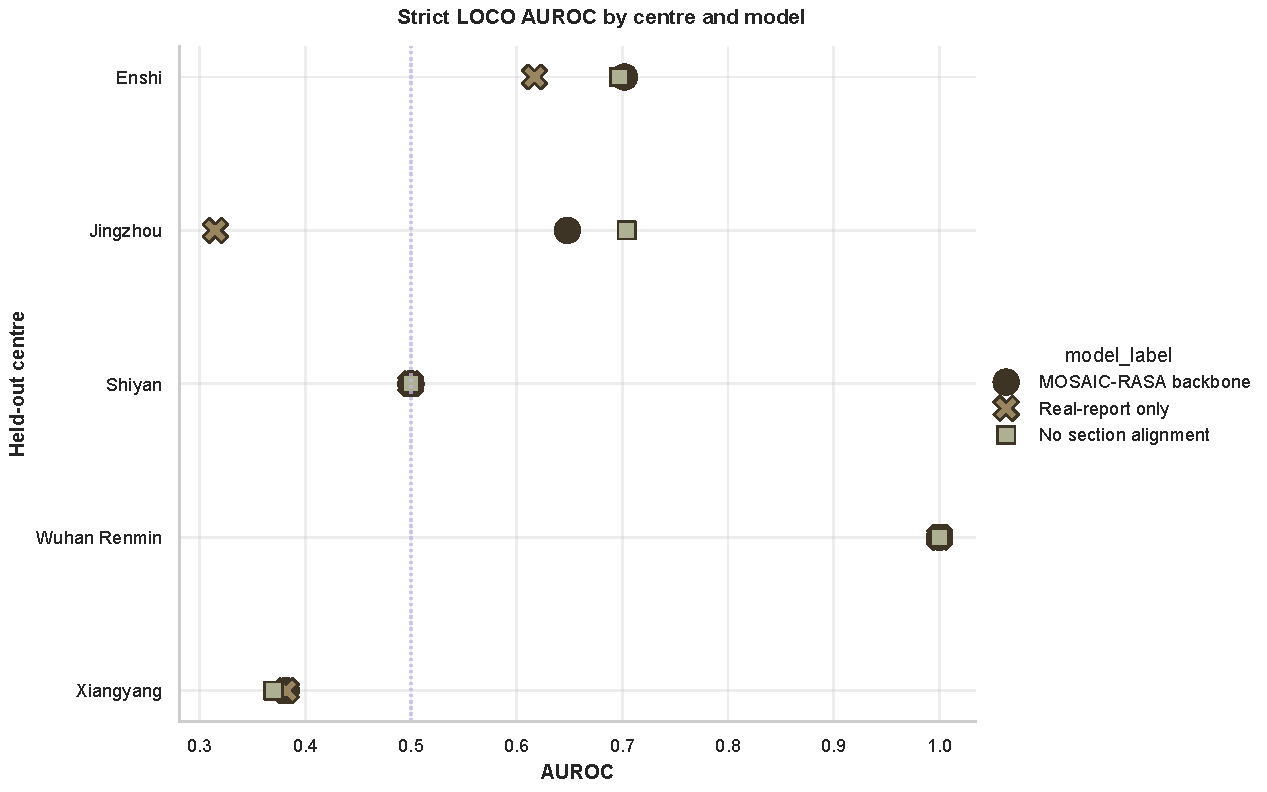
\includegraphics[width=1\linewidth]{final_Fig/fig_loco_heatmap.pdf}
%   \caption{Supplementary leave-one-centre-out evaluation across participating centres. The panels summarise centre-wise AUROC patterns and strict LOCO performance, illustrating the extent of distribution shift under centre-held-out evaluation.}
%   \label{app:fig:loco_heatmap}
% \end{figure}

% \subsection{Strict LOCO forest plot}
% \label{app:subsec:loco_forest}
% \begin{figure}[!htbp]
%   \centering
%   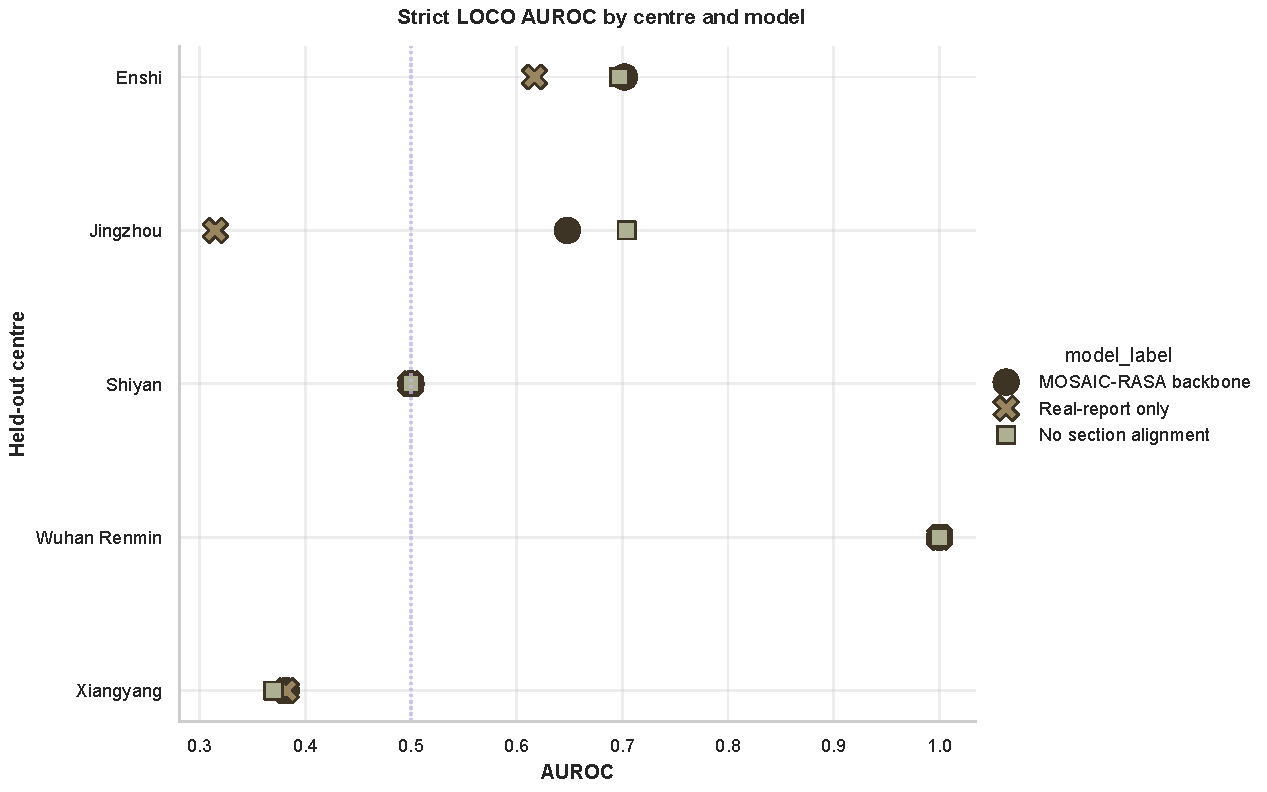
\includegraphics[width=\linewidth]{final_Fig/Figure4_loco_forest_catplot.pdf}
%   \caption{Supplementary strict leave-one-centre-out behaviour under fixed quick-budget retraining. Centre-wise estimates characterise how MOSAIC-RASA backbone and comparator variants perform when each centre is held out during model fitting.}
%   \label{app:fig:loco_forest}
% \end{figure}

% \subsection{Multi-seed stability of backbone variants}
% \label{app:subsec:multiseed_stability}
% \begin{table*}[!htbp]
%   \centering
%   \caption{Supplementary Table S7. Multi-seed AUROC stability.}
%   \label{app:tab:s7_multiseed_stability}
%   \scriptsize
%   \begin{threeparttable}
%   \resizebox{\linewidth}{!}{%
%   \begin{tabular}{lrrr}
%     \toprule
%     \textbf{Model} & \textbf{Mean AUROC} & \textbf{95\% interval} & \textbf{SD} \\
%     \midrule
%     MOSAIC-RASA backbone                    & \underline{0.776} & [0.773, 0.781] & 0.004 \\
%     Report generation without section alignment & \textbf{0.780} & [0.767, 0.795] & 0.012 \\
%     Real-report-only decoder                 & 0.667 & [0.656, 0.679] & 0.010 \\
%     \bottomrule
%   \end{tabular}%
%   }
%   \begin{tablenotes}[flushleft]
%     \footnotesize
%     \item The original metric-by-row table contained several constant rows. Across all seeds and models, mean F1 was 0.510, section completeness was 1.000, hallucination rate was 0.000, and label consistency was 0.641; the table therefore reports the variable stability metric, AUROC.
%   \end{tablenotes}
%   \end{threeparttable}
% \end{table*}

% \subsection{Report-level safety indicators}
% \label{app:subsec:report_safety}
% \begin{table*}[!htbp]
%   \centering
%   \caption{Supplementary Table S9. Report-level safety metrics.}
%   \label{app:tab:s9_report_safety_metrics}
%   \scriptsize
%   \begin{threeparttable}
%   \resizebox{\linewidth}{!}{%
%   \begin{tabular}{lrrrrr}
%     \toprule
%     \textbf{Evaluated settings} & \textbf{\makecell{Missing-modality\\hallucination}} & \textbf{\makecell{Label-report\\contradiction}} & \textbf{\makecell{Recommendation\\contradiction}} & \textbf{\makecell{Section\\incompleteness}} & \textbf{\makecell{Any\\hallucination}} \\
%     \midrule
%     \makecell[l]{Real-report-only decoder;\\Simple concatenation fusion;\\No section alignment;\\MOSAIC-RASA backbone;\\Pseudo reports, no QC;\\QC-confidence weighted pseudo reports}
%     & 0.000 & 0.847 & 0.000 & 0.000 & 0.000 \\
%     \bottomrule
%   \end{tabular}%
%   }
%   \begin{tablenotes}[flushleft]
%     \footnotesize
%     \item All evaluated settings had identical values in the current legacy rule-based safety table; duplicate rows were merged. The label-report contradiction scalar is definition-sensitive and is not used as a main-text safety endpoint. The refreshed failure-enriched QC stress test is reported as the primary report-safety filtering audit.
%   \end{tablenotes}
%   \end{threeparttable}
% \end{table*}

% \subsection{Masking validation across centres}
% \label{app:subsec:masking_validation}
% \begin{table*}[!htbp]
%   \centering
%   \caption{Supplementary Table S10. Masking validation across agent settings and centres.}
%   \label{app:tab:s10_masking_validation}
%   \scriptsize
%   \begin{threeparttable}
%   \resizebox{\linewidth}{!}{%
%   \begin{tabular}{llrrrrr}
%     \toprule
%     \textbf{Setting} & \textbf{Centre} & \textbf{$n$} & \textbf{Label consistency} & \textbf{ROUGE-L} & \textbf{BLEU} & \textbf{METEOR} \\
%     \midrule
%     \multirow{4}{*}{Label-only agent}
%       & Enshi                  & 406 & 0.659 & 0.152 & 0.081 & 0.124 \\
%       & Jingzhou               & 334 & 0.513 & 0.145 & 0.076 & 0.118 \\
%       & Xiangyang              & 4   & 0.500 & 0.150 & 0.080 & 0.120 \\
%       & Enshi--Jingzhou pooled & 740 & 0.593 & 0.149 & 0.079 & 0.121 \\
%     \addlinespace[2pt]
%     \multirow{4}{*}{\makecell[l]{Modality-only agent;\\Modality-plus-label agent}}
%       & Enshi                  & 406 & \textbf{0.746} & \textbf{0.251} & \textbf{0.152} & \textbf{0.203} \\
%       & Jingzhou               & 334 & 0.564 & 0.238 & 0.144 & 0.195 \\
%       & Xiangyang              & 4   & \underline{0.750} & 0.245 & 0.148 & 0.200 \\
%       & Enshi--Jingzhou pooled & 740 & 0.664 & \underline{0.246} & \underline{0.149} & \underline{0.198} \\
%     \bottomrule
%   \end{tabular}%
%   }
%   \begin{tablenotes}[flushleft]
%     \footnotesize
%     \item The modality-only and modality-plus-label agents produced identical values across centres; duplicate rows were merged.
%   \end{tablenotes}
%   \end{threeparttable}
% \end{table*}

% \subsection{Scalability and runtime summary}
% \label{app:subsec:scalability_runtime}
% \begin{table*}[!htbp]
%   \centering
%   \caption{Supplementary Table S11. Scalability and runtime summary.}
%   \label{app:tab:s11_scalability_runtime}
%   \scriptsize
%   \begin{threeparttable}
%   \resizebox{\linewidth}{!}{%
%   \begin{tabular}{lr}
%     \toprule
%     \textbf{Metric} & \textbf{Value} \\
%     \midrule
%     \multicolumn{2}{l}{\textbf{Cohort and image scale}} \\
%     Total cases & 1,897 \\
%     Total centres & 5 \\
%     Total images & 137,591 \\
%     OCT images & 129,030 \\
%     Colposcopy images & 8,561 \\
%     Mean images per case & 72.531 \\
%     Median images per case & 123 \\
%     Maximum images per case & 144 \\
%     Real-report cases & 744 \\
%     Pseudo-report cases & 1,153 \\
%     Missing-report rate & 0.608 \\
%     \addlinespace[2pt]
%     \multicolumn{2}{l}{\textbf{Storage and checkpoint size}} \\
%     Embedding storage & 47.349 MB \\
%     Embedding files & 5,691 \\
%     Publishable checkpoint size, MOSAIC-RASA backbone / pseudo-augmented / real-report-only & 79.882 MB \\
%     Publishable checkpoint size, simple fusion / fusion plus section alignment & 79.879 MB \\
%     \bottomrule
%   \end{tabular}%
%   }
%   \end{threeparttable}
% \end{table*}

% \subsection{Robustness figures for masking and seed stability}
% \label{app:subsec:robustness_figures}
% \begin{figure}[!htbp]
%   \centering
%   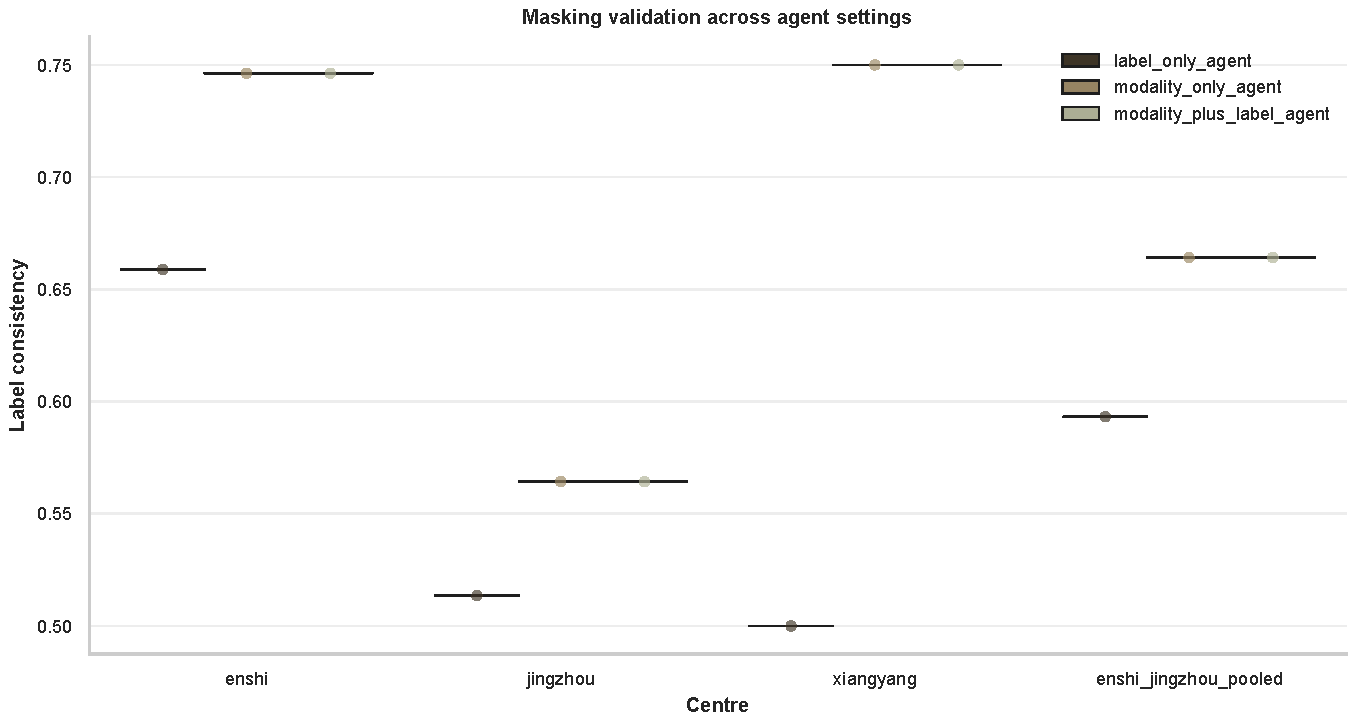
\includegraphics[width=\linewidth]{final_Fig/SupplementaryFigure_S1_masking_validation.pdf}
%   \hfill
%   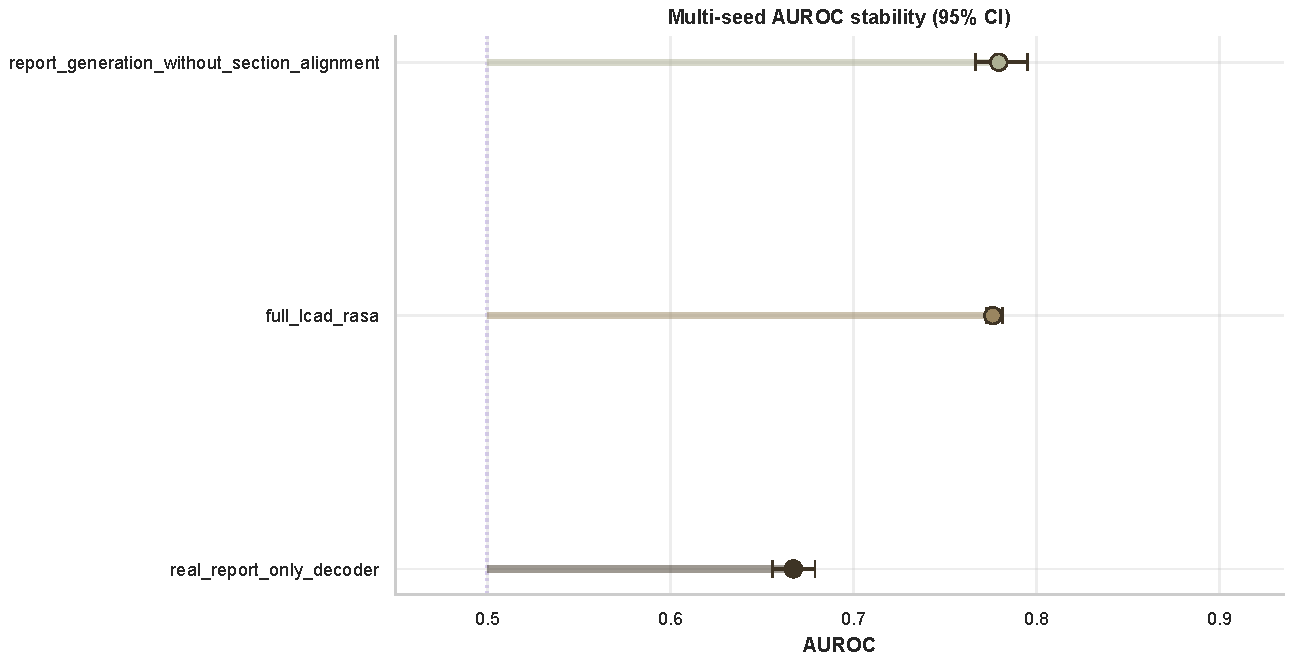
\includegraphics[width=\linewidth]{final_Fig/SupplementaryFigure_S3_multiseed.pdf}
%   \caption{Supplementary robustness analyses. The panels summarise masking-validation behaviour and multi-seed stability, providing additional evidence on reproducibility and sensitivity of the retrospective pipeline.}
%   \label{app:fig:supplementary_robustness}
% \end{figure}
% % END INTEGRATED_SUPPLEMENTARY_APPENDIX


% % \section{Section title of first appendix}\label{secA1}



% % \end{appendices}
% \section{List of abbreviations}

% \begin{tabular}{ll}
% AI & Artificial intelligence \\
% AUPRC & Area under the precision--recall curve \\
% AUROC & Area under the receiver operating characteristic curve \\
% CI & Confidence interval \\
% CIN2+ & Cervical intraepithelial neoplasia grade 2 or worse \\
% CIN3+ & Cervical intraepithelial neoplasia grade 3 or worse \\
% CLIP & Contrastive Language--Image Pre-training \\
% ECE & Expected calibration error \\
% F1 & Harmonic mean of precision and recall \\
% HPV & Human papillomavirus \\
% LCAD & Label-constrained and evidence-aware pseudo-report completion \\
% LLM & Large language model \\
% LOCO & Leave-one-centre-out \\
% MOSAIC & Multicentre Offline Structured Anchoring with Imbalanced-report Calibration \\
% MRR & Mean reciprocal rank \\
% OCT & Optical coherence tomography \\
% QC & Quality control \\
% RASA & Report-Anchored Structured Alignment \\
% TCT & ThinPrep cytologic test \\
% \end{tabular}


\bibliographystyle{unsrt}
\bibliography{sn-bibliography}% common bib file
%% if required, the content of .bbl file can be included here once bbl is generated
% \input sn-article.bbl


\end{document}
